\documentclass[../DoAn.tex]{subfiles}
\begin{document}

\section{Thiết kế kiến trúc}
\label{section:4.1}
\subsection{Lựa chọn kiến trúc phần mềm}
\label{subsection:4.1.1}
Microservices là một kiến trúc phần mềm mà trong đó một ứng dụng được xây dựng thành nhiều dịch vụ nhỏ, chúng được mô hình hoá xoay quanh những nhóm nghiệp vụ cụ thể.
Kiến trúc này là một kiểu của kiến trúc hướng dịch vụ (Service-Oriented Architecture - SOA), các dịch vụ nhỏ được thiết kế để chạy trên các luồng độc lập, song song
với nhau, chúng kết hợp với nhau để thực thi một luồng nghiệp vụ, giao tiếp qua lại thông qua một mạng kết nối riêng.\cite{MicroservicesPatterns}

Kiến trúc Microservices có hai mục tiêu chính là tính độc lập triển khai và mô hình hoá dựa trên nghiệp vụ. Cụ thể, tính độc lập triển khai được thể hiện ở điểm:
mỗi dịch vụ khi cần thay thế, nâng cấp hay sửa lỗi thì nhà phát triển có thể thực thi điều đó mà không ảnh hưởng đến các dịch vụ khác. Đối với các dịch vụ,
phạm vi của chúng được giới hạn bởi một nghiệp vụ cụ thể, chúng quản lý dữ liệu của riêng mình, điều này rất tương đồng với mô hình Domain Driven Design (DDD).\cite{BuildingMicroservices}

Về ưu điểm, kiến trúc Microservices giúp cho việc phát triển ứng dụng trở nên đơn giản hơn, mỗi dịch vụ có thể được phát triển độc lập bởi một đội ngũ phát triển riêng,
với ngôn ngữ lập trình riêng. Họ có thể lựa chọn chọn công nghệ phù hợp với từng loại nghiệp vụ mà không bị ràng buộc bởi các dịch vụ khác.\cite{BuildingMicroservices}

Do các dịch vụ là độc lập với nhau, việc triển khai mã nguồn, mở rộng theo chiều ngang có thể được thực hiện riêng rẽ, hoàn toàn dựa trên yêu cầu của từng dịch vụ.
Ví dụ, một dịch vụ có lượng truy cập cao đột ngột có thể được mở rộng bằng cách nhân thêm các bản sao của chính nó, có thể phát sinh lỗi và dừng hoạt động mà không ảnh hưởng
tới tất cả các thành phần khác trong hệ thống.\cite{BuildingMicroservices}

Trong phạm vi dự án, em lựa chọn kiến trúc Microservices để xây dựng hệ thống quản lý dự án. Các dịch vụ được chia nhỏ như sau:
\begin{itemize}
    \item Dịch vụ xác thực và quản lý tài khoản (Identity Server): xác thực người dùng, phân quyền người dùng.
    \item Dịch vụ quản lý người dùng (Personal Data Service): quản lý thông tin cá nhân của người dùng, thông tin về tổ chức, đội nhóm.
    \item Dịch vụ quản lý dự án (Portal Service): quản lý thông tin dự án, quản lý công việc, quản lý tài liệu.
    \item Dịch vụ giao tiếp (Communication Service): gửi thông báo, gửi thư điện tử.
    \item Dịch vụ dữ liệu chủ (Master Data Service): quản lý dữ liệu chung của hệ thống.
    \item Hàng đợi tin nhắn (Message Queue): một trong những phương thức giao tiếp giữa các dịch vụ, gửi tin nhắn bất đồng bộ.
    \item Cơ sở dữ liệu (Database): chứa các bảng dữ liệu của hệ thống.
    \item Cơ sở dữ liệu tạm thời (Temporary Database): chứa các bảng dữ liệu tạm thời của hệ thống.
    \item Cổng giao tiếp (Gateway): tập hợp điểm cuối của hệ thống, nhận các yêu cầu từ người dùng và gửi tới các dịch vụ phù hợp.
\end{itemize}

Ngoài ra, hệ thống cũng chứa các thành phần khác phục vụ cho quá trình phát triển và vận hành hệ thống, cụ thể như quản lý log, mã hoá dữ liệu nhạy cảm, quản lý chứng chỉ số,
quản lý hiệu năng và mức độ tiêu thụ tài nguyên hệ thống.

\begin{figure}[H]
    \centering
    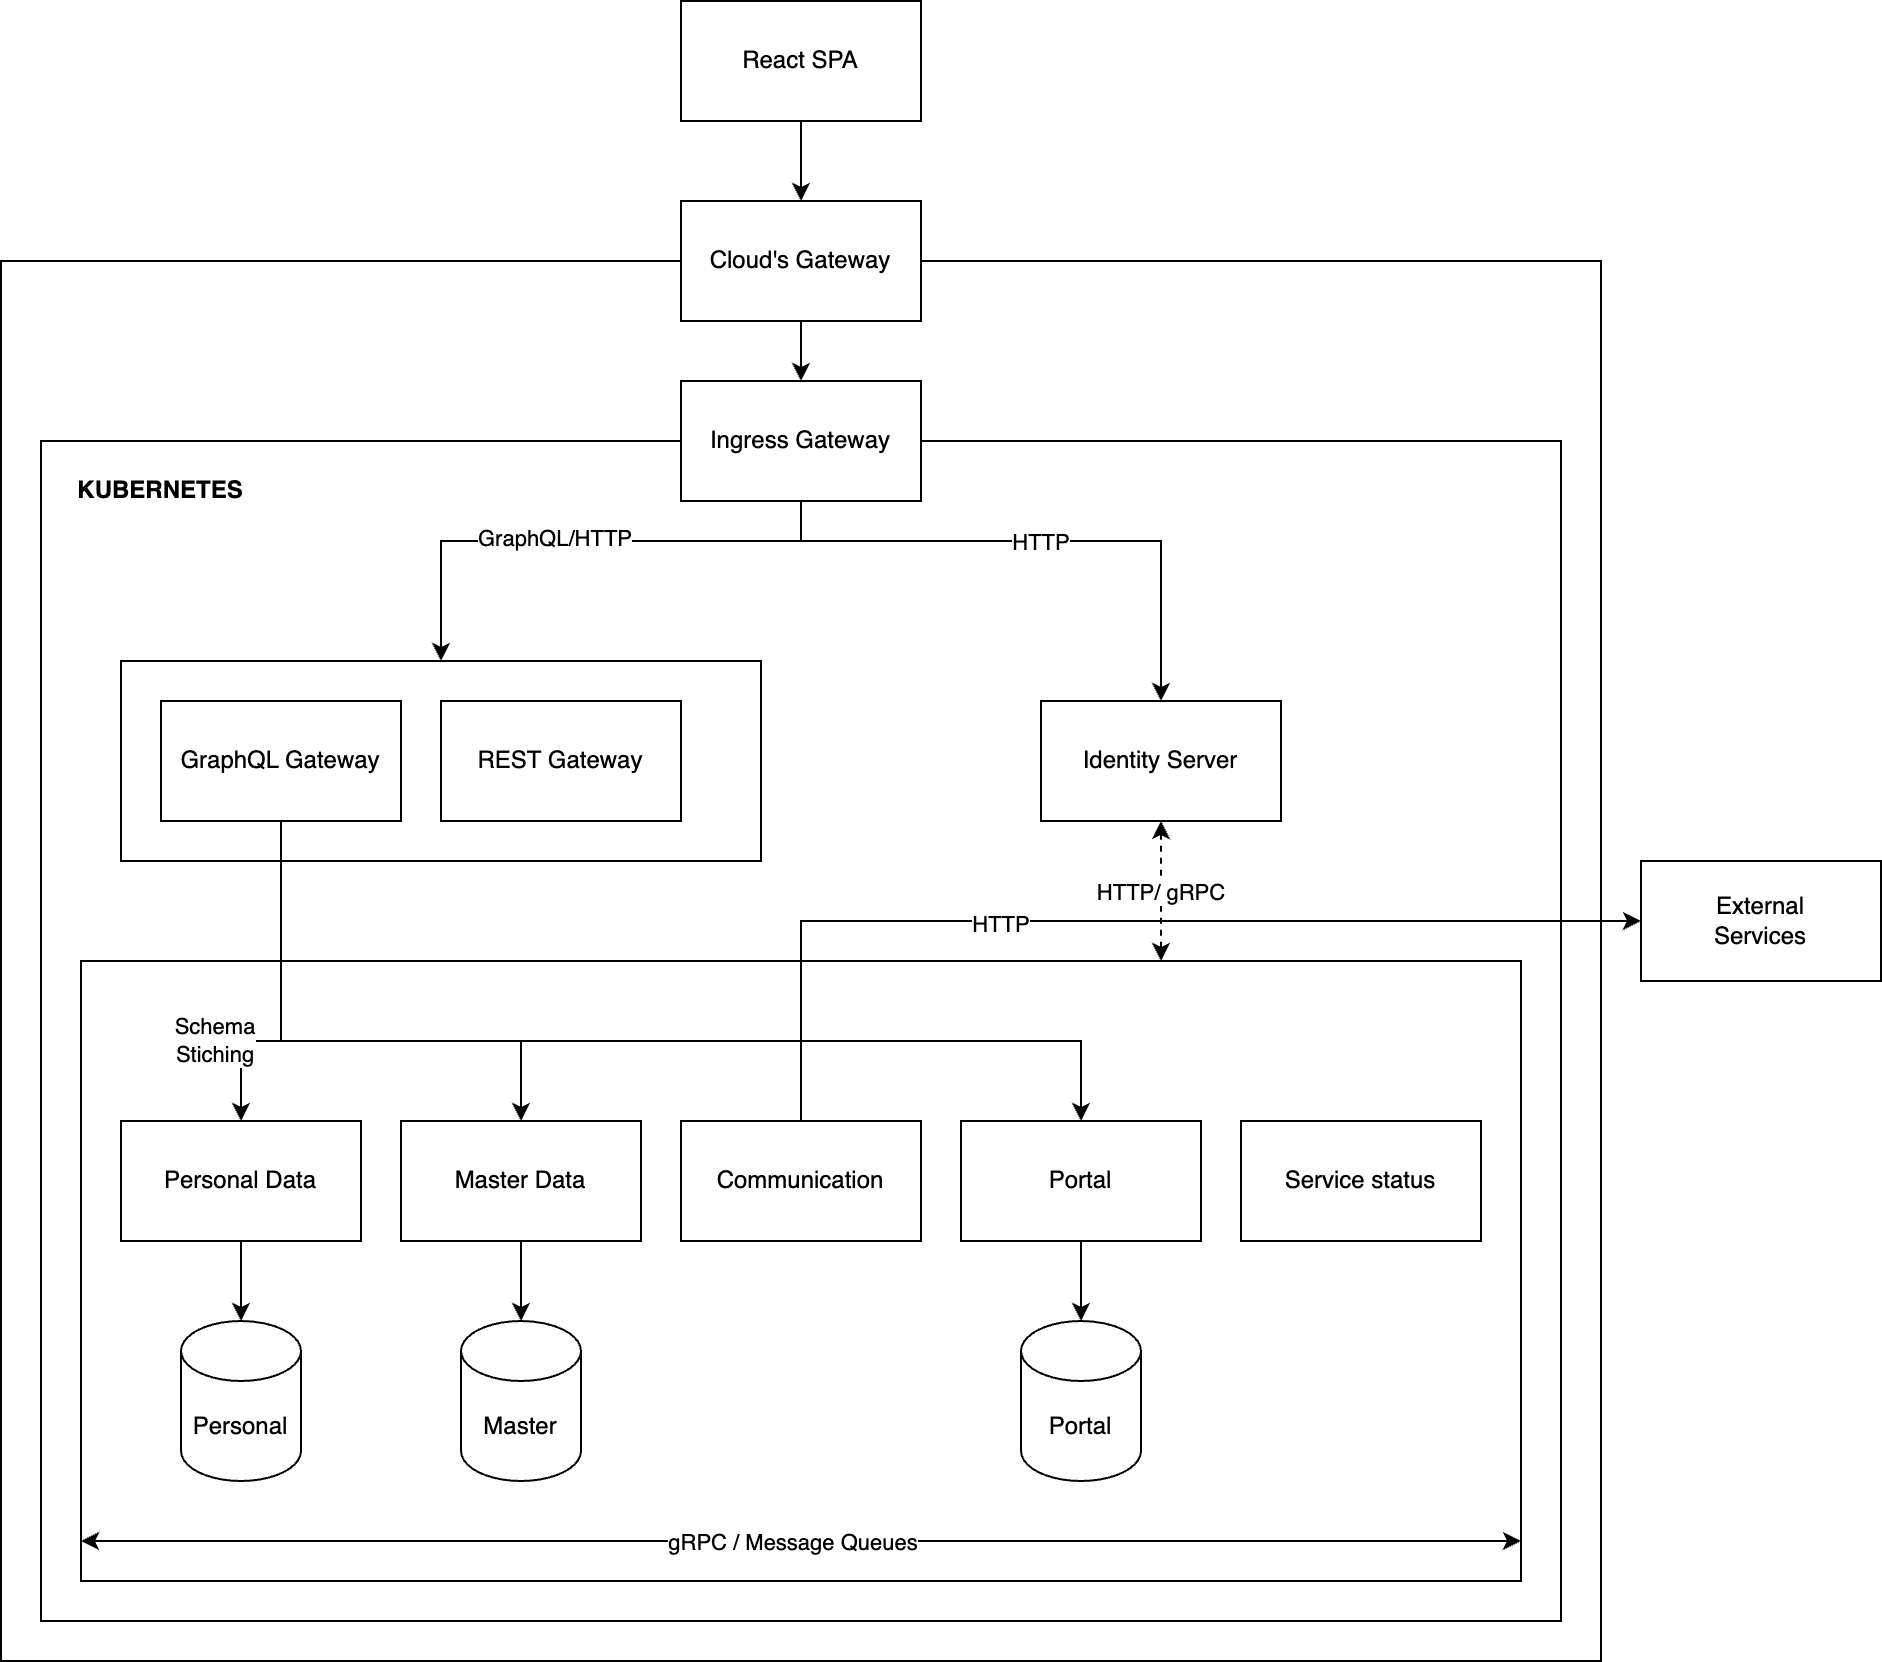
\includegraphics[width=1.0\linewidth]{Hinhve/MicroserviceArchitecture.png}
    \caption{Hình minh hoạ các thành phần của hệ thống dựa trên kiến trúc Microservices}
    \label{fig:MicroserviceArchitecture}
\end{figure}
\newpage

\subsection{Thiết kế tổng quan}
\label{subsection:4.1.2}
Đối với một hệ thống sử dụng kiến trúc Microservice, các dịch vụ được chia nhỏ và hoạt động độc lập với nhau, mối liên hệ giữa chúng được thể hiện qua giao tiếp bằng giao diện (interface)
hay hợp đồng (contract) được định nghĩa trước. Biểu đồ thành phần dưới đây thể hiện mối quan hệ giữa các dịch vụ với nhau.

Với ba dịch vụ chính là Portal, Master Data và Personal Data,
chúng đều có một cơ sở dữ liệu riêng, các điểm cuối (Endpoint) của chúng được định nghĩa trước, quản lý bởi một cổng giao tiếp (API Gateway) và xác thực bởi dịch vụ quản lý tài khoản (Identity Server).
Dịch vụ giao tiếp (Communication) được kết nối với một dịch vụ gửi thư điện tử và xác thực bởi Identity Server.

Gateway tổng hợp định nghĩa của các điểm cuối (endpoint) của các dịch vụ, giao tiếp với Internet để gửi và nhận yêu cầu từ bên ngoài vào trong hệ thống và ngược lại. Ngoài ra,
Gateway còn thực hiện nhiệm vụ điều tiết yêu cầu, quyết định việc tạo thêm bản sao của các dịch vụ khi hệ thống gặp nguy cơ quá tải.

Tương tự, Identity Server cũng đảm nhiệm vai trò như Gateway đối với các yêu cầu về xác thực và phân quyền, ngoài ra dịch vụ này cũng quản lý các thông tin về tài khoản người dùng,
phiên đăng nhập và các thông tin liên quan.

\begin{figure}[H]
    \centering
    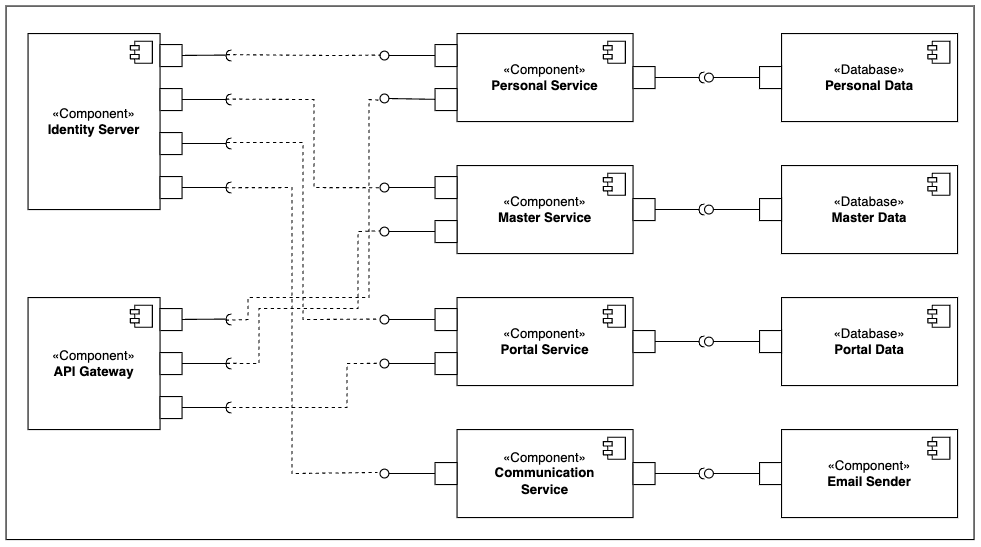
\includegraphics[width=1.0\linewidth]{Hinhve/General_ComponentDiagram.png}
    \caption{Biểu đồ thành phần của hệ thống}
    \label{fig:General_ComponentDiagram}
\end{figure}
\newpage


\subsection{Thiết kế chi tiết gói}
\label{subsection:4.1.3}

Với mỗi dịch vụ trong hệ thống, các thành phần được chia nhỏ thành các gói (package), mỗi gói chứa các lớp, giao diện có cùng vai trò với nhau.
Các gói này được phân chia dựa trên mẫu thiết kế Mediator (Mediator Pattern) cùng với đặc điểm của kiến trúc Microservices, mỗi dịch vụ có nhiều
điểm cuối và phương thức gửi/nhận yêu cầu khác nhau tuỳ theo mục đích sử dụng.

\begin{figure}[H]
    \centering
    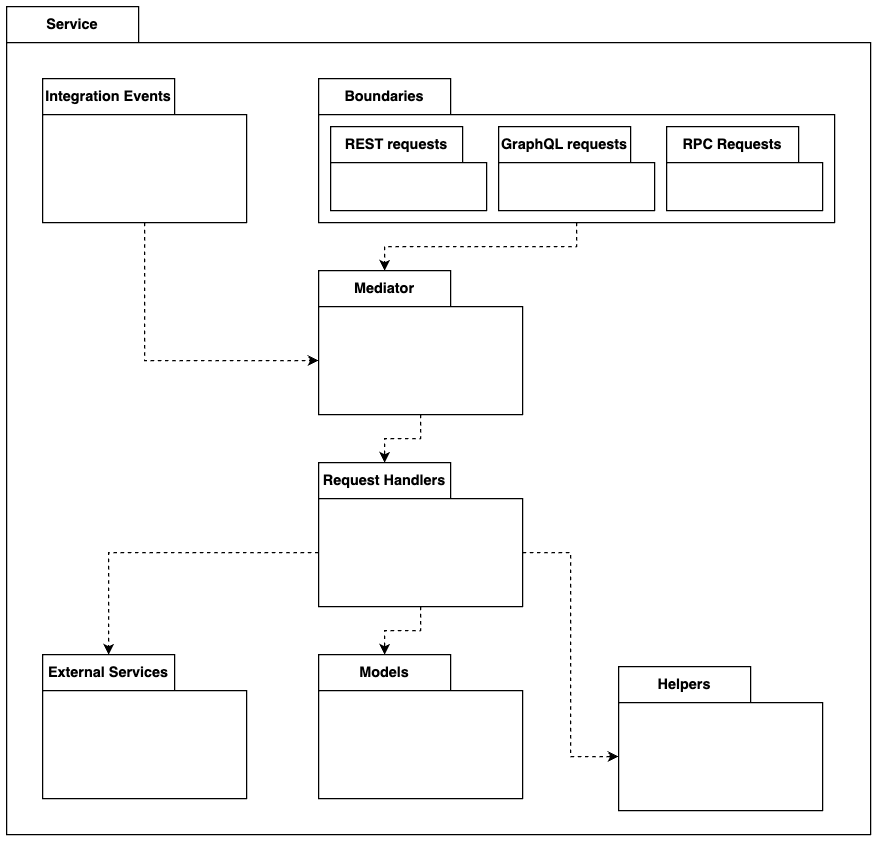
\includegraphics[width=1.0\linewidth]{Hinhve/Package_GeneralServicePackageDiagram.png}
    \caption{Biểu đồ gói tổng quát của các dịch vụ trong hệ thống}
    \label{fig:Package_GeneralServicePackageDiagram}
\end{figure}

Cụ thể, mỗi dịch vụ thường cung cấp bốn loại yêu cầu tương ứng với bốn loại điểm cuối khác nhau, bao gồm: Integration Event thông qua Message Queue,
các yêu cầu thông qua giao thức RESTful API, GraphQL API và RPC. Chúng đều được tiếp nhận và gửi tới gói Mediator, gói này có nhiệm vụ điều tiết yêu cầu
tới các lớp xử lý tương ứng (Handler Class). Các lớp này có nhiệm vụ xử lý yêu cầu, truy xuất dữ liệu từ cơ sở dữ liệu, liên lạc tới các dịch vụ khác và gửi lại kết quả cho gói Mediator.

\newpage

Mediator là một mẫu thiết kế hành vi (Behavioral Pattern), nó cho phép giảm sự phụ thuộc giữa các đối tượng trong một hệ thống phần mềm bằng cách
giúp chúng giao tiếp với nhau thông qua một đối tượng trung gian duy nhất. Mẫu thiết kế này giúp giảm sự phụ thuộc giữa các lớp, đồng thời giúp cho việc
mở rộng hệ thống trở nên dễ dàng hơn. Hơn nữa, một luồng yêu cầu khi được triển khai sẽ tường minh hơn, tập các đối tượng sử dụng cũng dễ dàng để liệt kê.\cite{DesignPatterns}

Cụ thể, mẫu thiết kế này có hai thành phần chính là Mediator và Request, chúng là các giao diện (interface) được định nghĩa trước nhằm chỉ ra cách
giao tiếp giữa các request với nhau và với đối tượng trung gian Mediator. Concrete Mediator là lớp triển khai giao diện Mediator, nó chứa thông tin về tất cả
các lớp triển khai giao diện Request, đồng thời cũng chứa các phương thức để điều tiết các yêu cầu tới các lớp xử lý tương ứng. Request Handler là lớp triển khai
giao diện Request, nó chứa trạng thái cụ thể của đối tượng cũng như các phương thức để xử lý yêu cầu đó.

\begin{figure}[H]
    \centering
    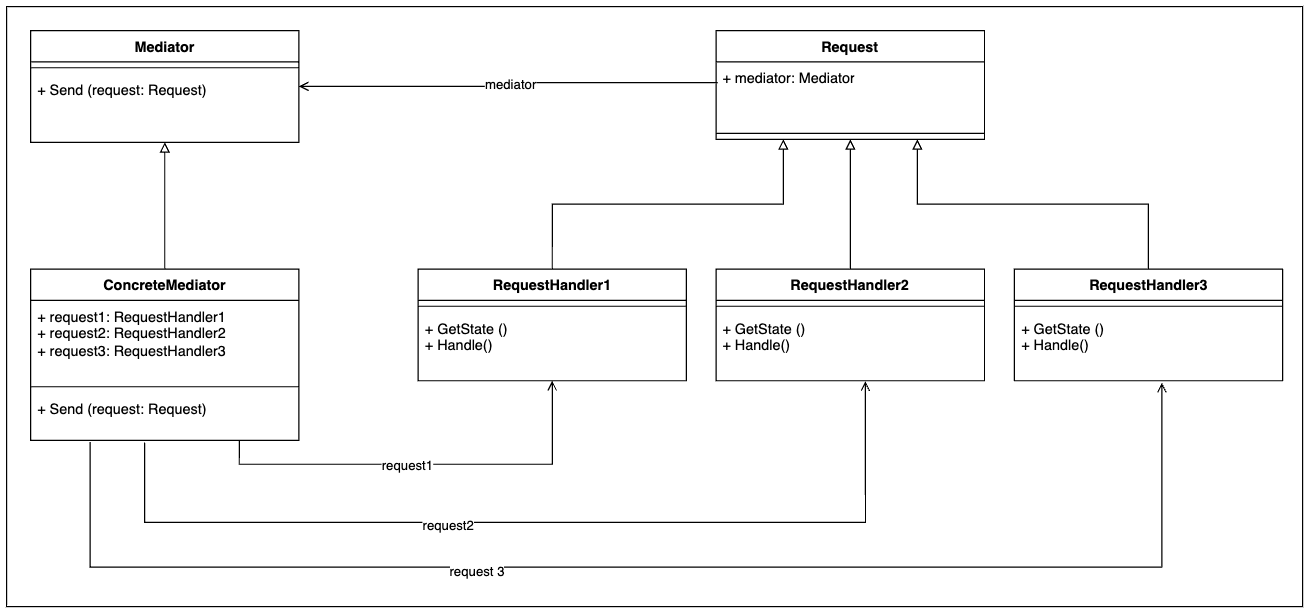
\includegraphics[width=1.0\linewidth]{Hinhve/ClassDiagram_Mediator.png}
    \caption{Biểu đồ lớp của gói Mediator}
    \label{fig:ClassDiagram_Mediator}
\end{figure}

Ngoài Mediator, các gói khác đều định nghĩa các lớp xoay quanh các yêu cầu (Request) và các lớp xử lý yêu cầu (Request Handler). Chúng không có mối liên hệ trực tiếp
nào với nhau mà chỉ phục vụ giải quyết một nghiệp vụ cụ thể. Ngoại trừ gói Model, chúng chứa các lớp là đối tượng của các thực thể trong cơ sở dữ liệu, các lớp này
có mối quan hệ tương tự như các bảng trong cơ sở dữ liệu.

\newpage


\section{Thiết kế chi tiết}
\label{section:4.2}
\subsection{Thiết kế giao diện}
\label{subsection:4.2.1}
\begin{figure}[H]
    \centering
    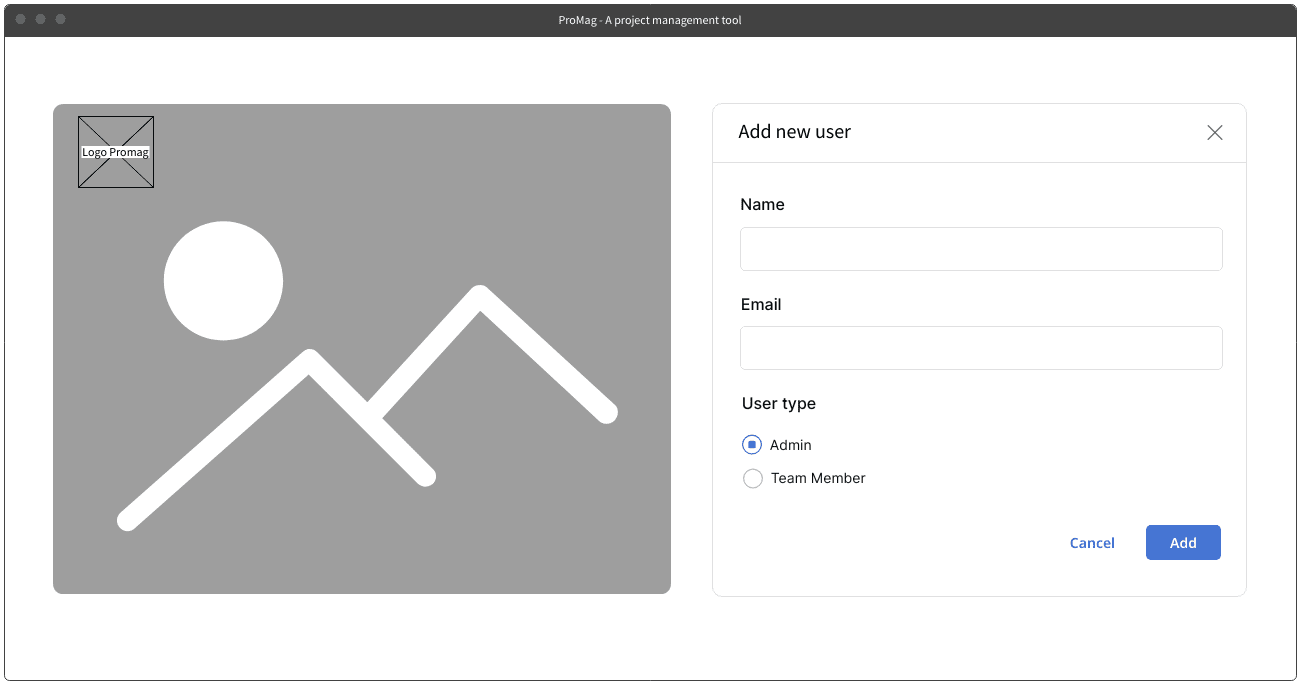
\includegraphics[width=1.0\linewidth]{Hinhve/Mockup_Register.png}
    \caption{Thiết kế giao diện Đăng ký}
    \label{fig:Mockup_Register}
\end{figure}

\begin{figure}[H]
    \centering
    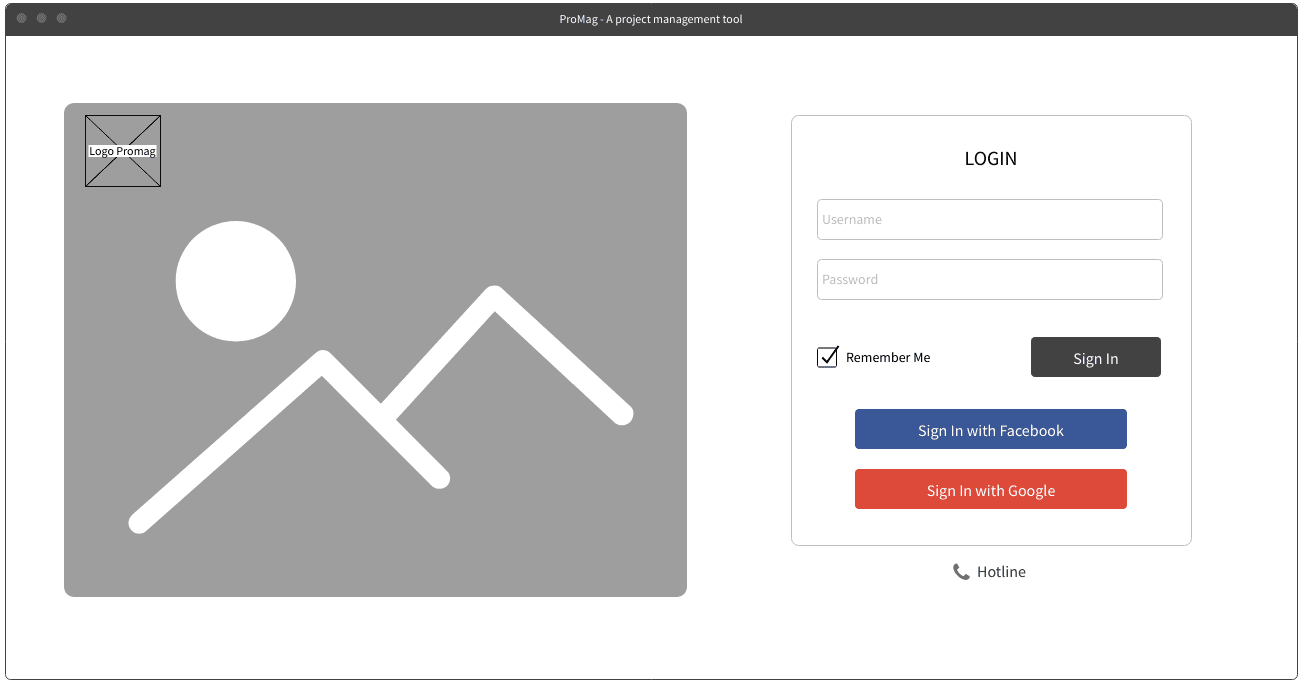
\includegraphics[width=1.0\linewidth]{Hinhve/Mockup_Login.png}
    \caption{Thiết kế giao diện Đăng nhập}
    \label{fig:Mockup_Login}
\end{figure}

\newpage

\begin{figure}[H]
    \centering
    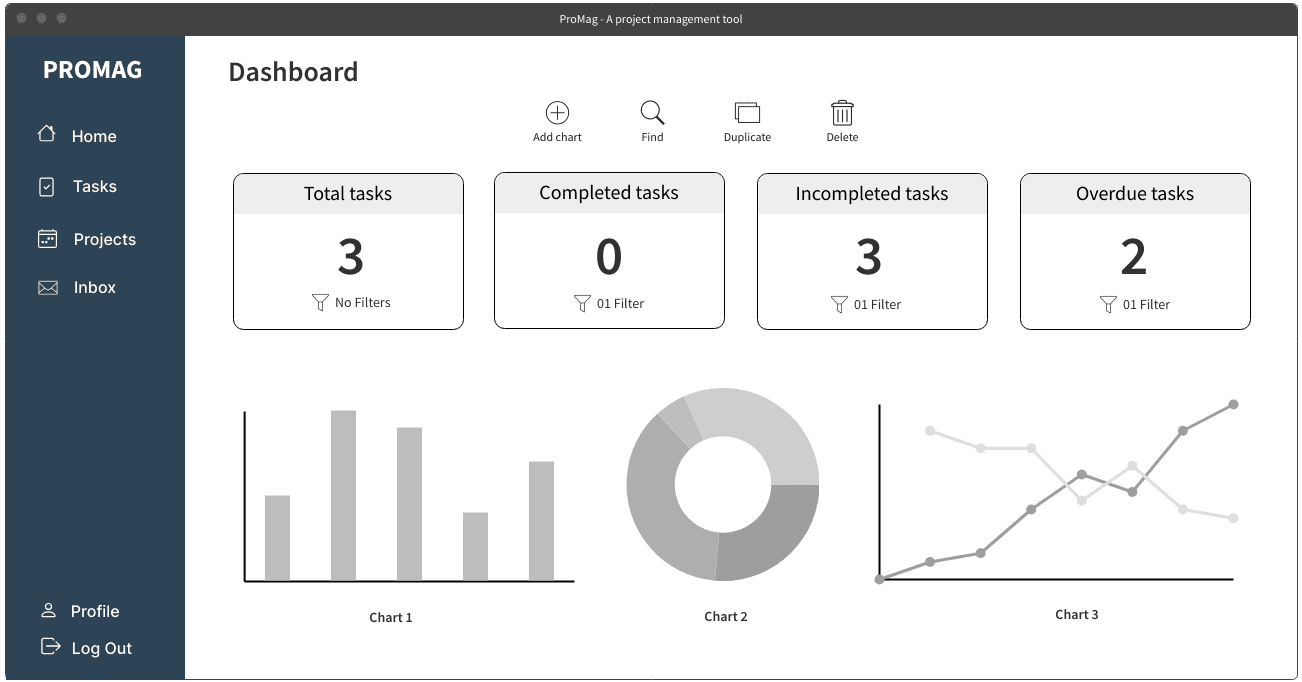
\includegraphics[width=1.0\linewidth]{Hinhve/Mockup_Dashboard.png}
    \caption{Thiết kế giao diện Thống kê}
    \label{fig:Mockup_Dashboard}
\end{figure}

\begin{figure}[H]
    \centering
    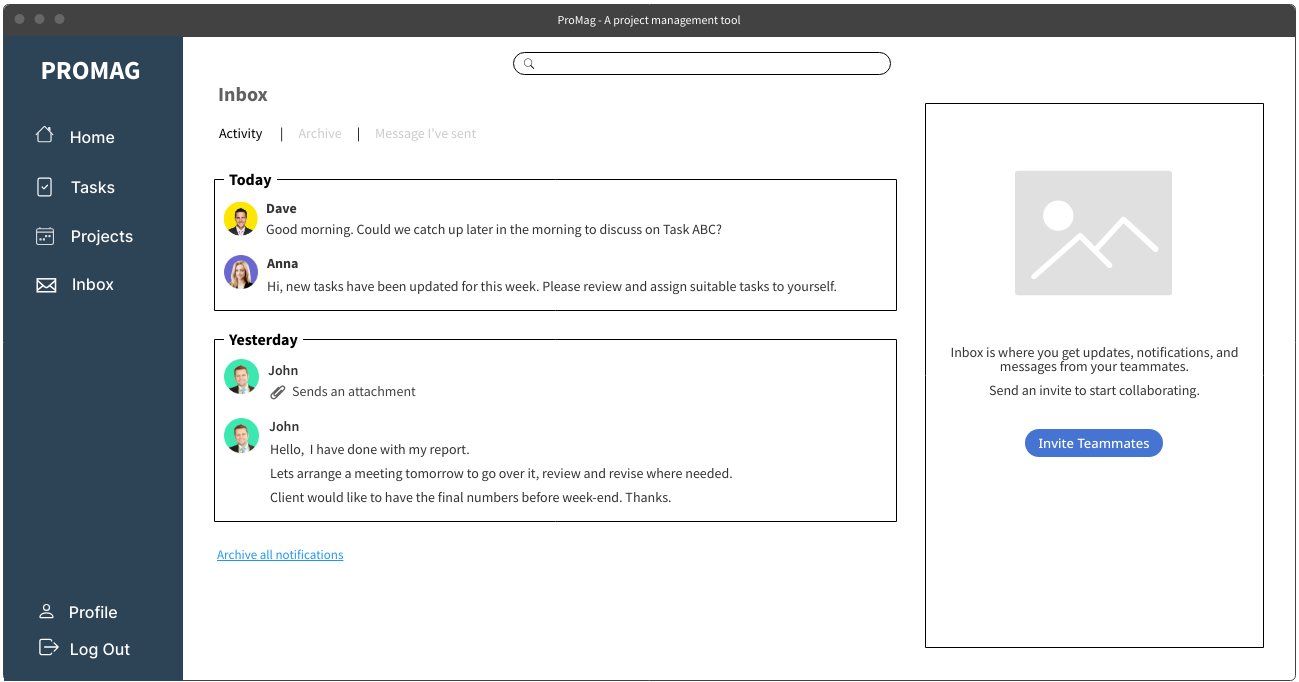
\includegraphics[width=1.0\linewidth]{Hinhve/Mockup_Inbox.png}
    \caption{Thiết kế giao diện Hộp thông báo}
    \label{fig:Mockup_Inbox}
\end{figure}

\newpage

\begin{figure}[H]
    \centering
    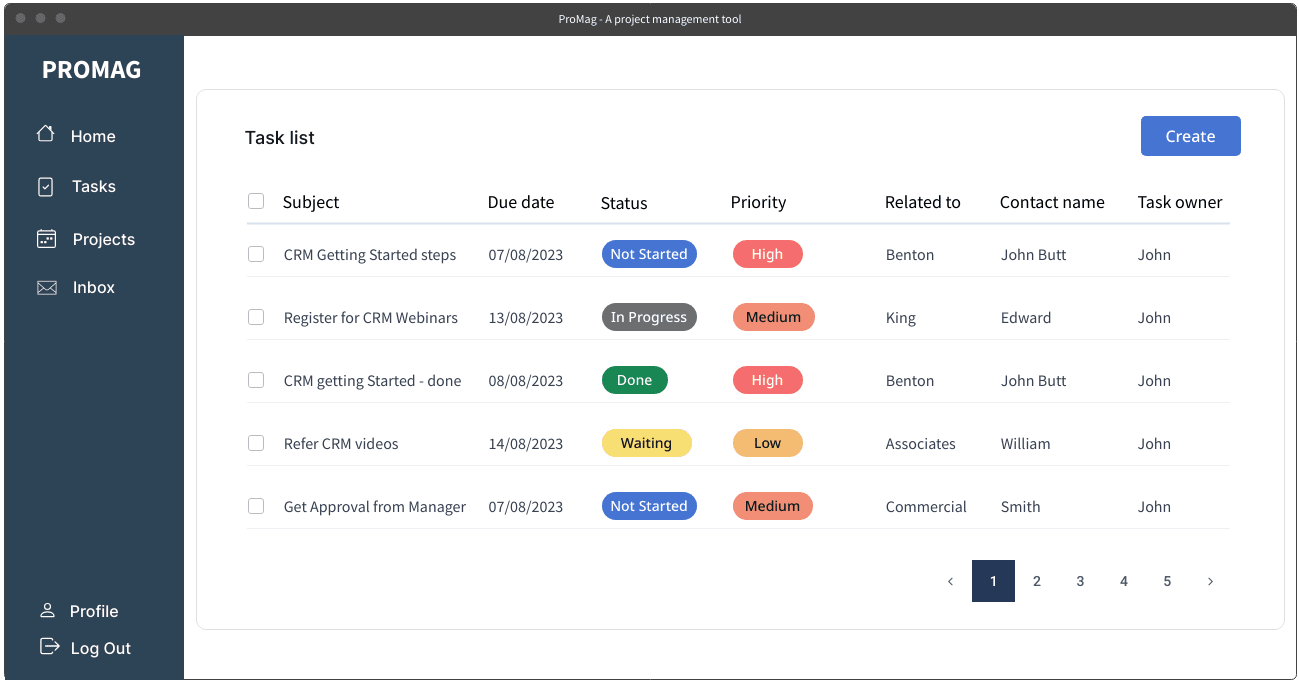
\includegraphics[width=1.0\linewidth]{Hinhve/Mockup_AllTaskList.png}
    \caption{Thiết kế giao diện Danh sách tất cả công việc}
    \label{fig:Mockup_AllTaskList}
\end{figure}

\begin{figure}[H]
    \centering
    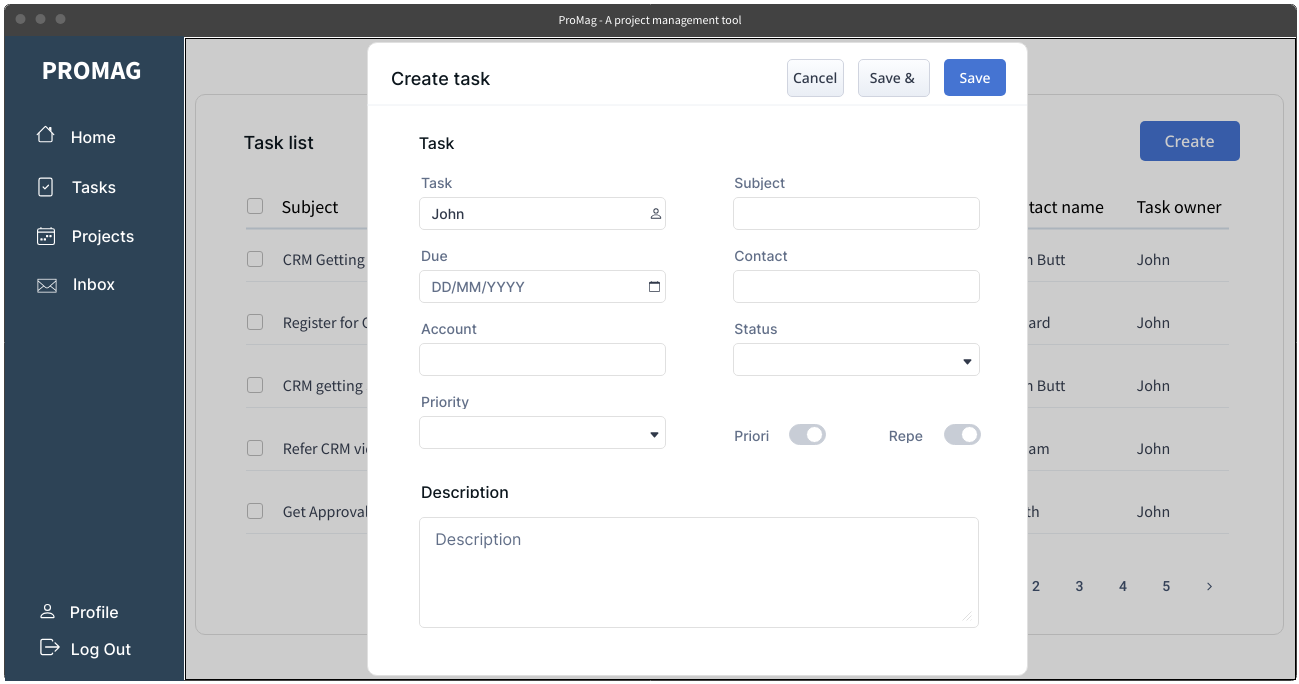
\includegraphics[width=1.0\linewidth]{Hinhve/Mockup_CreateTask.png}
    \caption{Thiết kế giao diện Tạo công việc}
    \label{fig:Mockup_CreateTask}
\end{figure}

\newpage

\begin{figure}[H]
    \centering
    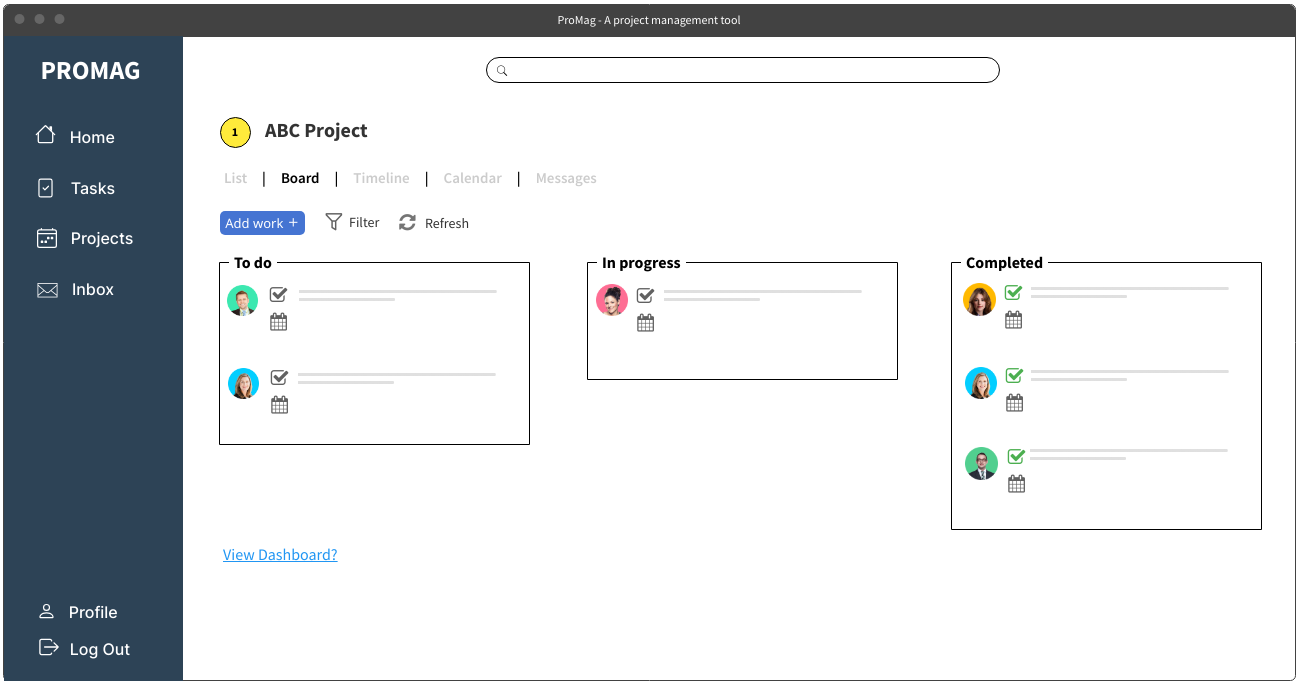
\includegraphics[width=1.0\linewidth]{Hinhve/Mockup_Kanban.png}
    \caption{Thiết kế giao diện Chi tiết dự án dạng bảng Kanban}
    \label{fig:Mockup_Kanban}
\end{figure}

\begin{figure}[H]
    \centering
    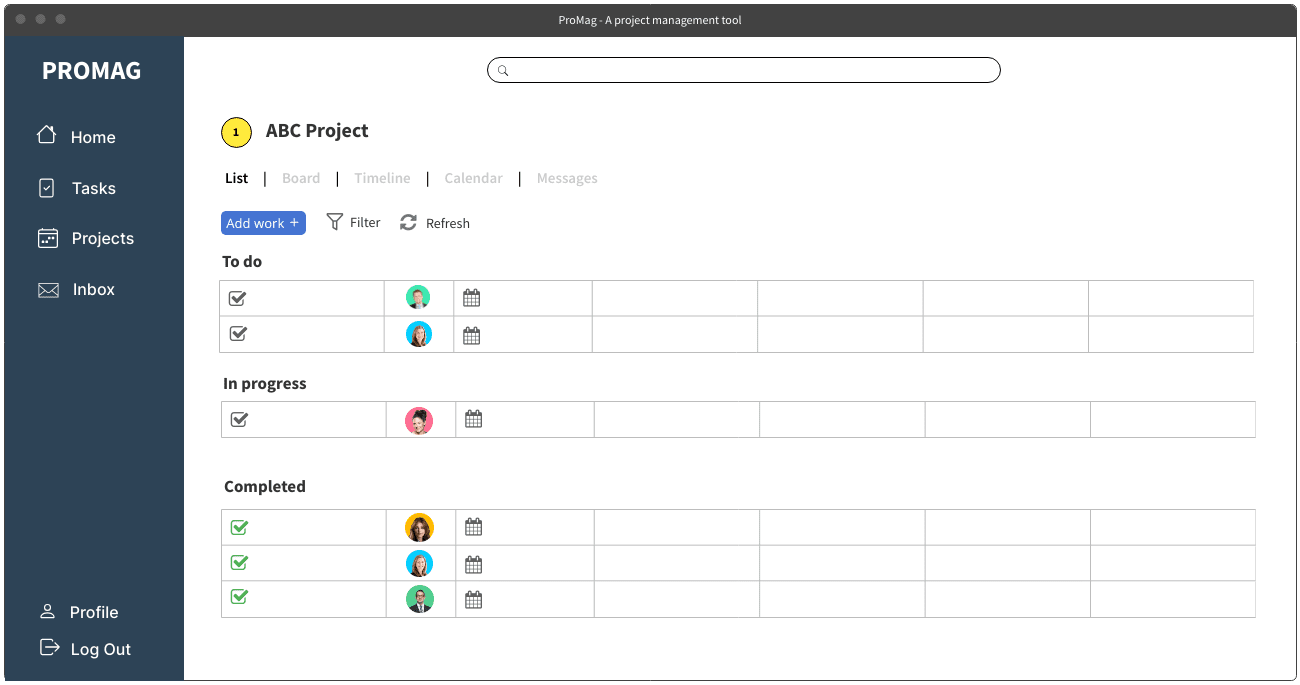
\includegraphics[width=1.0\linewidth]{Hinhve/Mockup_TaskList.png}
    \caption{Thiết kế giao diện Chi tiết dự án dạng danh sách}
    \label{fig:Mockup_TaskList}
\end{figure}

\newpage

\begin{figure}[H]
    \centering
    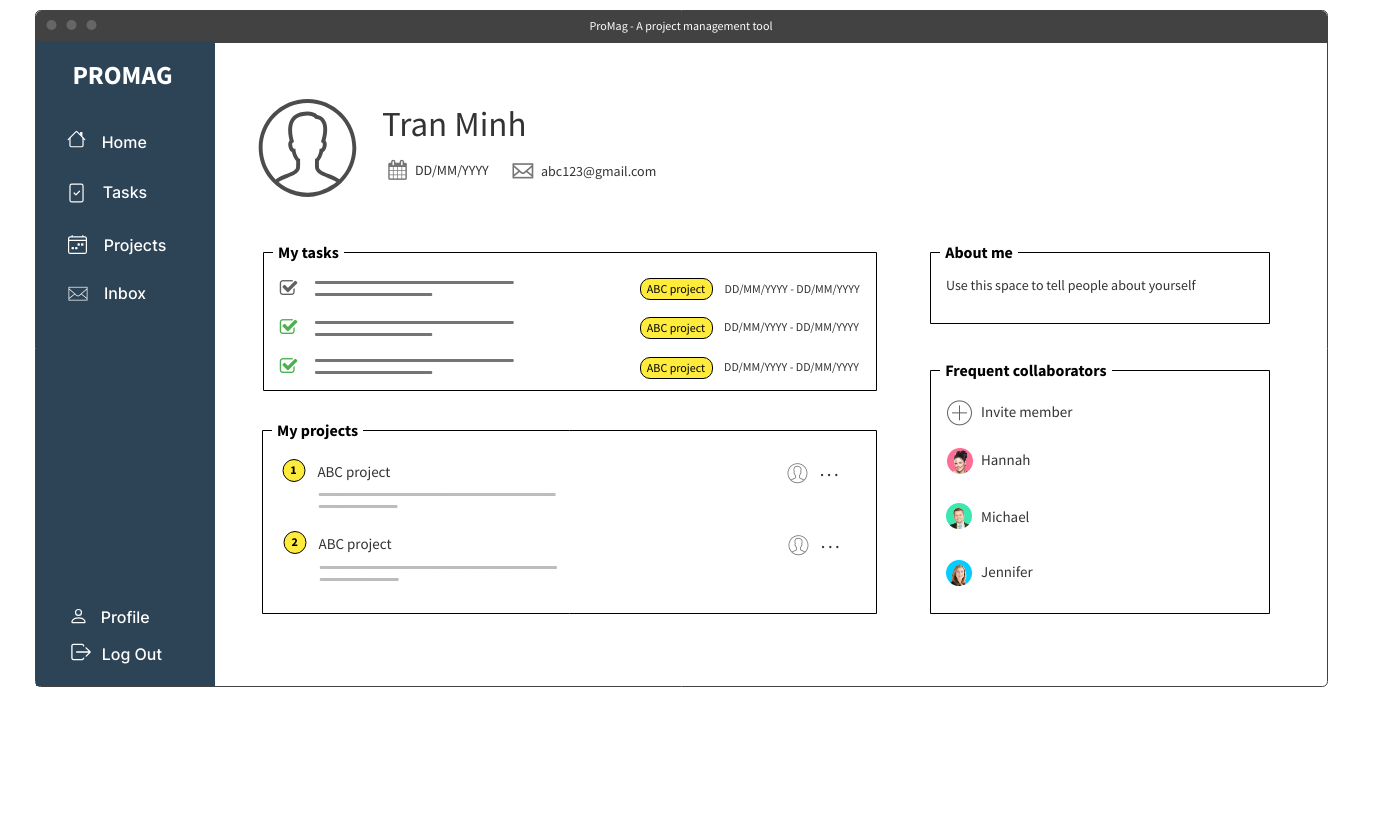
\includegraphics[width=1.0\linewidth]{Hinhve/Mockup_Profile.png}
    \caption{Thiết kế giao diện Hồ sơ của tôi}
    \label{fig:Mockup_Profile}
\end{figure}

\begin{figure}[H]
    \centering
    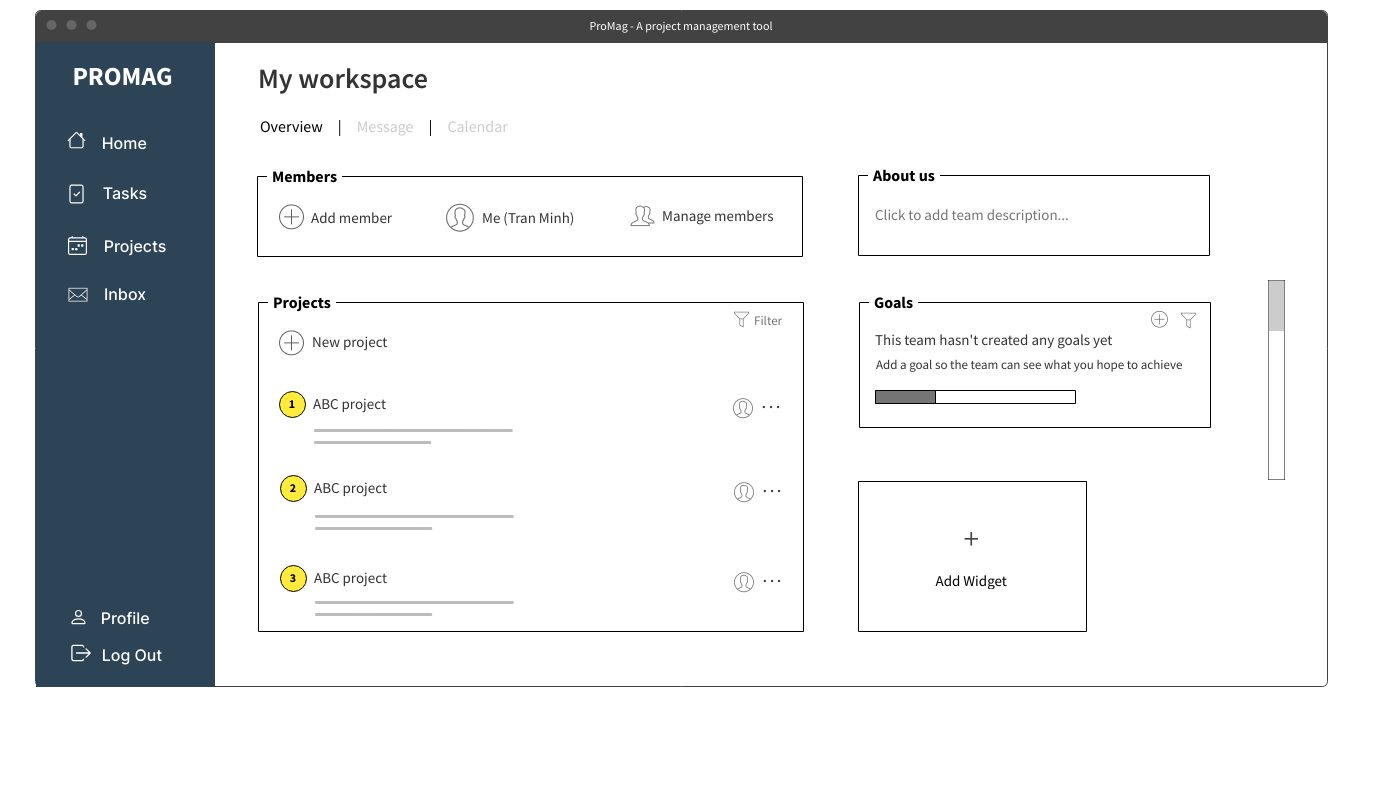
\includegraphics[width=1.0\linewidth]{Hinhve/Mockup_MyWorkspace.png}
    \caption{Thiết kế giao diện Chi tiết không gian làm việc nhóm}
    \label{fig:Mockup_MyWorkspace}
\end{figure}

\newpage

\subsection{Thiết kế lớp}
\label{subsection:4.2.2}

Đầu tiên, em xin đưa ra thiết kế chi tiết cho 2 lớp chính liên quan đến người dùng là User và Person.
Lớp User là lớp đại diện cho người dùng trong hệ thống, chứa các thông tin về tài khoản. Lớp Person là lớp đại diện cho thông tin
cá nhân của người dùng, chứa các thông tin như họ tên, địa chỉ, số điện thoại. Chúng có quan hệ 1-1 với nhau.

\begin{table}[H]
    \renewcommand{\arraystretch}{1.2}
    \centering{}
    \begin{tabular}{p{0.3\linewidth}p{0.2\linewidth}p{0.5\linewidth}}
        \hline
        \textbf{Tên}                     & \textbf{Kiểu dữ liệu} & \textbf{Mô tả}                                      \\ \hline
        \textbf{Thuộc tính}                                                                                            \\ \hline
        Id                               & Unique Identifier     & Định danh duy nhất của mỗi bản ghi                  \\ \hline
        Username                         & String                & Tên đăng nhập của User                              \\ \hline
        Email                            & String                & Địa chỉ email duy nhất của User                     \\ \hline
        EmailConfirmed                   & Boolean               & Cờ xác định User đã xác thực địa chỉ email hay chưa \\ \hline
        PasswordHash                     & String                & Mật khẩu của User sau khi đi qua hàm băm            \\ \hline
        LockoutEnabled                   & Boolean               & Cờ xác định User có đang bị khoá tạm thời không     \\ \hline
        LockoutEnd                       & DateTime              & Thời điểm User được gỡ khoá tạm thời                \\ \hline
        AccessFailedCount                & Integer               & Số lần User thử đăng nhập và thất bại               \\ \hline
        \textbf{Phương thức}                                                                                           \\ \hline
        HashPassword(string password)    & Boolean               & Băm mật khẩu của User đã nhập                       \\ \hline
        ComparePassword(string password) & Boolean               & Kiểm tra mật khẩu có đúng hay không                 \\ \hline
        LockAccount()                    & Void                  & Khoá tài khoản của User                             \\ \hline
        UnlockAccount()                  & Void                  & Mở khoá tài khoản của User                          \\ \hline
    \end{tabular}
    \renewcommand{\arraystretch}{1}
    \caption{Thiết kế chi tiết lớp User}
    \label{fig:classdesign_user}
\end{table}

\newpage

\begin{table}[H]
    \renewcommand{\arraystretch}{1.2}
    \centering{}
    \begin{tabular}{p{0.3\linewidth}p{0.2\linewidth}p{0.5\linewidth}}
        \hline
        \textbf{Tên}                & \textbf{Kiểu dữ liệu} & \textbf{Mô tả}                       \\ \hline
        \textbf{Thuộc tính}                                                                        \\ \hline
        Id                          & Unique Identifier     & Định danh duy nhất của mỗi bản ghi   \\ \hline
        UserId                      & Unique Identifier     & Định danh duy nhất của User          \\ \hline
        FirstName                   & String                & Tên của User                         \\ \hline
        LastName                    & String                & Họ và tên đệm của User               \\ \hline
        PhotoPath                   & String                & Đường dẫn tới hình đại diện của User \\ \hline
        MobilePhone                 & String                & Số điện thoại của User               \\ \hline
        \textbf{Phương thức}                                                                       \\ \hline
        SetAvatar(string photoPath) & Void                  & Cập nhật hình đại diện của User      \\ \hline
    \end{tabular}
    \renewcommand{\arraystretch}{1}
    \caption{Thiết kế chi tiết lớp Person}
    \label{fig:classdesign_person}
\end{table}

Dưới đây là biểu đồ tuần tự cho luồng Đăng ký tài khoản, trong đó có sử dụng các lớp User và Person đã thiết kế ở trên.
Về cơ bản, khi một người dùng đăng ký tài khoản sẽ tạo ra hai bản ghi tương ứng trong hai bảng User và Person có liên kết 1-1 với nhau.
Nhằm đảm bảo địa chỉ email của người dùng chính xác và mật khẩu được đảm bảo an toàn, hệ thống sẽ gửi một thư điện tử xác nhận tới địa chỉ email của người dùng.

\begin{figure}[H]
    \centering
    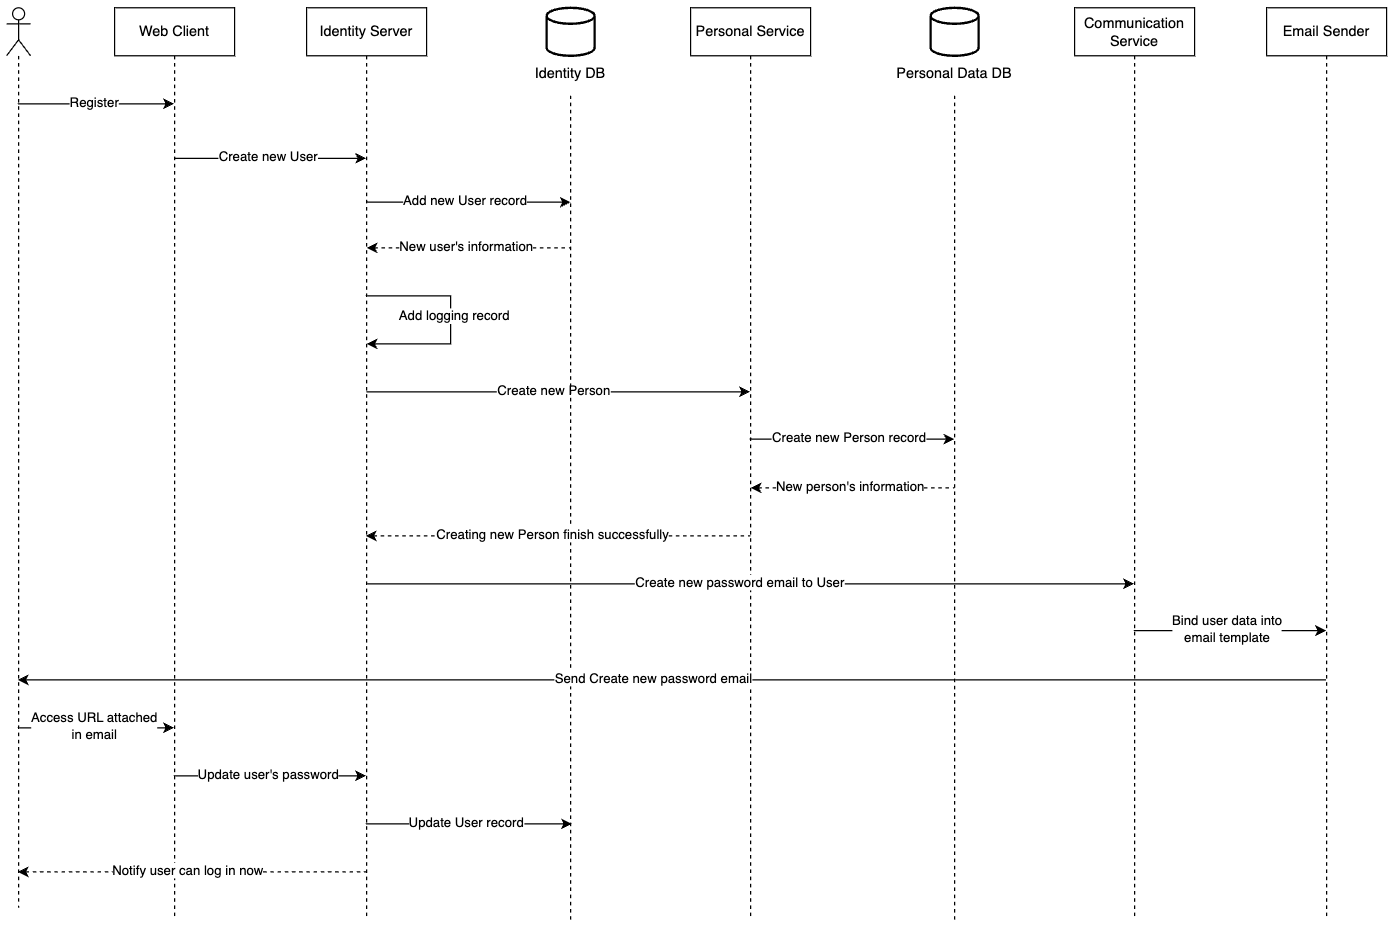
\includegraphics[width=1.0\linewidth]{Hinhve/SequenceDiagram_Register.png}
    \caption{Biểu đồ tuần tự luồng Đăng ký}
    \label{fig:SequenceDiagram_Register}
\end{figure}

\newpage

Tiếp đến, em xin trình bày thiết kế chi tiết cho các lớp chính liên quan đến dự án là Project, Section và Task. Các lớp này được thiết
kế để phù hợp với giao diện bảng Kanban, trong đó mỗi dự án (Project) sẽ có một bảng Kanban riêng,
bao gồm các cột (Section) tương ứng với các trạng thái công việc.

\begin{table}[H]
    \renewcommand{\arraystretch}{1.2}
    \centering{}
    \begin{tabular}{p{0.3\linewidth}p{0.2\linewidth}p{0.5\linewidth}}
        \hline
        \textbf{Tên} & \textbf{Kiểu dữ liệu} & \textbf{Mô tả}                                      \\ \hline
        \textbf{Thuộc tính}                                                                        \\ \hline
        Id           & Unique Identifier     & Định danh duy nhất của mỗi bản ghi                  \\ \hline
        Name         & String                & Tên dự án                                           \\ \hline
        Notes        & String                & Mô tả về dự án                                      \\ \hline
        DueDate      & DateTime              & Ngày tới hạn của dự án                              \\ \hline
        Archived     & Boolean               & Cờ xác định dự án có ở trạng thái lưu trữ hay không \\ \hline
        OwnerId      & Unique Identifier     & Định danh duy nhất của User tạo ra dự án            \\ \hline
        WorkspaceId  & Unique Identifier     & Định danh duy nhất của không gian làm việc          \\ \hline
        TeamId       & Unique Identifier     & Định danh duy nhất của nhóm thực hiện dự án         \\ \hline
        \textbf{Phương thức}                                                                       \\ \hline
        Archive()    & Void                  & Đưa dự án vào trạng thái lưu trữ                    \\ \hline
    \end{tabular}
    \renewcommand{\arraystretch}{1}
    \caption{Thiết kế chi tiết lớp Project}
    \label{fig:classdesign_project}
\end{table}

\begin{table}[H]
    \renewcommand{\arraystretch}{1.2}
    \centering{}
    \begin{tabular}{p{0.3\linewidth}p{0.2\linewidth}p{0.5\linewidth}}
        \hline
        \textbf{Tên}                & \textbf{Kiểu dữ liệu} & \textbf{Mô tả}                        \\ \hline
        \textbf{Thuộc tính}                                                                         \\ \hline
        Id                          & Unique Identifier     & Định danh duy nhất của mỗi bản ghi    \\ \hline
        Name                        & String                & Tên cột Kanban (trạng thái công việc) \\ \hline
        ProjectId                   & Unique Identifier     & Định danh duy nhất của dự án          \\ \hline
        OrderIndex                  & Integer               & Vị trí của cột trên bảng Kanban       \\ \hline
        \textbf{Phương thức}                                                                        \\ \hline
        UpdateName(string newName)  & String                & Cập nhật tên trạng thái               \\ \hline
        MoveColumn(int newPosition) & Void                  & Cập nhật vị trí cột trên bảng Kanban  \\ \hline
    \end{tabular}
    \renewcommand{\arraystretch}{1}
    \caption{Thiết kế chi tiết lớp Section}
    \label{fig:classdesign_section}
\end{table}

\newpage

\begin{table}[H]
    \renewcommand{\arraystretch}{1.2}
    \centering{}
    \begin{tabular}{p{0.3\linewidth}p{0.2\linewidth}p{0.5\linewidth}}
        \hline
        \textbf{Tên}                  & \textbf{Kiểu dữ liệu} & \textbf{Mô tả}                                  \\ \hline
        \textbf{Thuộc tính}                                                                                     \\ \hline
        Id                            & Unique Identifier     & Định danh duy nhất của mỗi bản ghi              \\ \hline
        Name                          & String                & Tên công việc                                   \\ \hline
        Notes                         & String                & Mô tả về công việc                              \\ \hline
        StartDate                     & DateTime              & Ngày bắt đầu của công việc                      \\ \hline
        DueDate                       & DateTime              & Ngày tới hạn của công việc                      \\ \hline
        Completed                     & Boolean               & Cờ xác định công việc đã hoàn thành chưa        \\ \hline
        CompletedOn                   & DateTime              & Ngày hoàn thành của công việc                   \\ \hline
        CustomField                   & String                & Các trường dữ liệu khác                         \\ \hline
        ProjectId                     & Unique Identifier     & Định danh duy nhất của dự án                    \\ \hline
        SectionId                     & Unique Identifier     & Định danh duy nhất của cột Kanban               \\ \hline
        WorkspaceId                   & Unique Identifier     & Định danh duy nhất của không gian làm việc      \\ \hline
        AssigneeId                    & Unique Identifier     & Định danh duy nhất của User thực hiện công việc \\ \hline
        \textbf{Phương thức}                                                                                    \\ \hline
        Assign(string userId)         & Void                  & Giao công việc cho một User                     \\ \hline
        MoveToColum(string sectionId) & Void                  & Di chuyển công việc tới một cột Kanban khác     \\ \hline
        Complete()                    & Void                  & Hoàn thành công việc                            \\ \hline
    \end{tabular}
    \renewcommand{\arraystretch}{1}
    \caption{Thiết kế chi tiết lớp Task}
    \label{fig:classdesign_task}
\end{table}

\newpage

Dưới đây là biểu đồ tuần tự cho luồng Cập nhật thay đổi trong dự án, trong đó có sử dụng các lớp Project, Section và Task đã thiết kế ở trên.
Có rất nhiều loại thay đổi có thể xảy ra mà người dùng thao tác trên giao diện, nhưng cơ bản thì chúng đều tương tự nhau, đó là cập nhật lại thông tin
của các thực thể kể trên.


\begin{figure}[H]
    \centering
    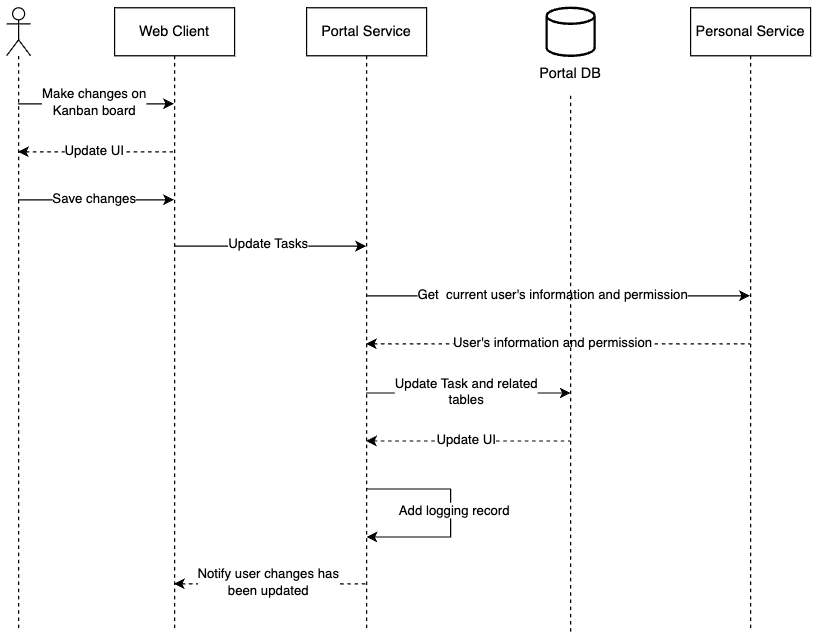
\includegraphics[width=1.0\linewidth]{Hinhve/SequenceDiagram_UpdateTask.png}
    \caption{Biểu đồ tuần tự luồng Cập nhật công việc}
    \label{fig:SequenceDiagram_Register}
\end{figure}

\newpage

\subsection{Thiết kế cơ sở dữ liệu}
\label{subsection:4.2.3}

Do hệ thống được xây dựng dựa trên kiến trúc Microservices, nên dữ liệu cũng được chia nhỏ thành các cơ sở dữ liệu khác nhau, dưới đây là thiết kế cơ sở dữ liệu của
hai dịch vụ chính là Portal và Personal. Các dịch vụ khác không cần thiết sử dụng cơ sở dữ liệu để lưu trữ.

Cơ sở dữ liệu của dịch vụ Portal được thiết kế gồm các bảng chính là Projects, Tasks, Sections, Stories, Attachments và Tags. Các bảng này tương ứng với các thực thể
trong tầng ứng dụng của dịch vụ Portal. Các bảng còn lại là các bảng phụ, có tác dụng liên kết, bổ sung thông tin cho các bảng chính.

\begin{figure}[H]
    \centering
    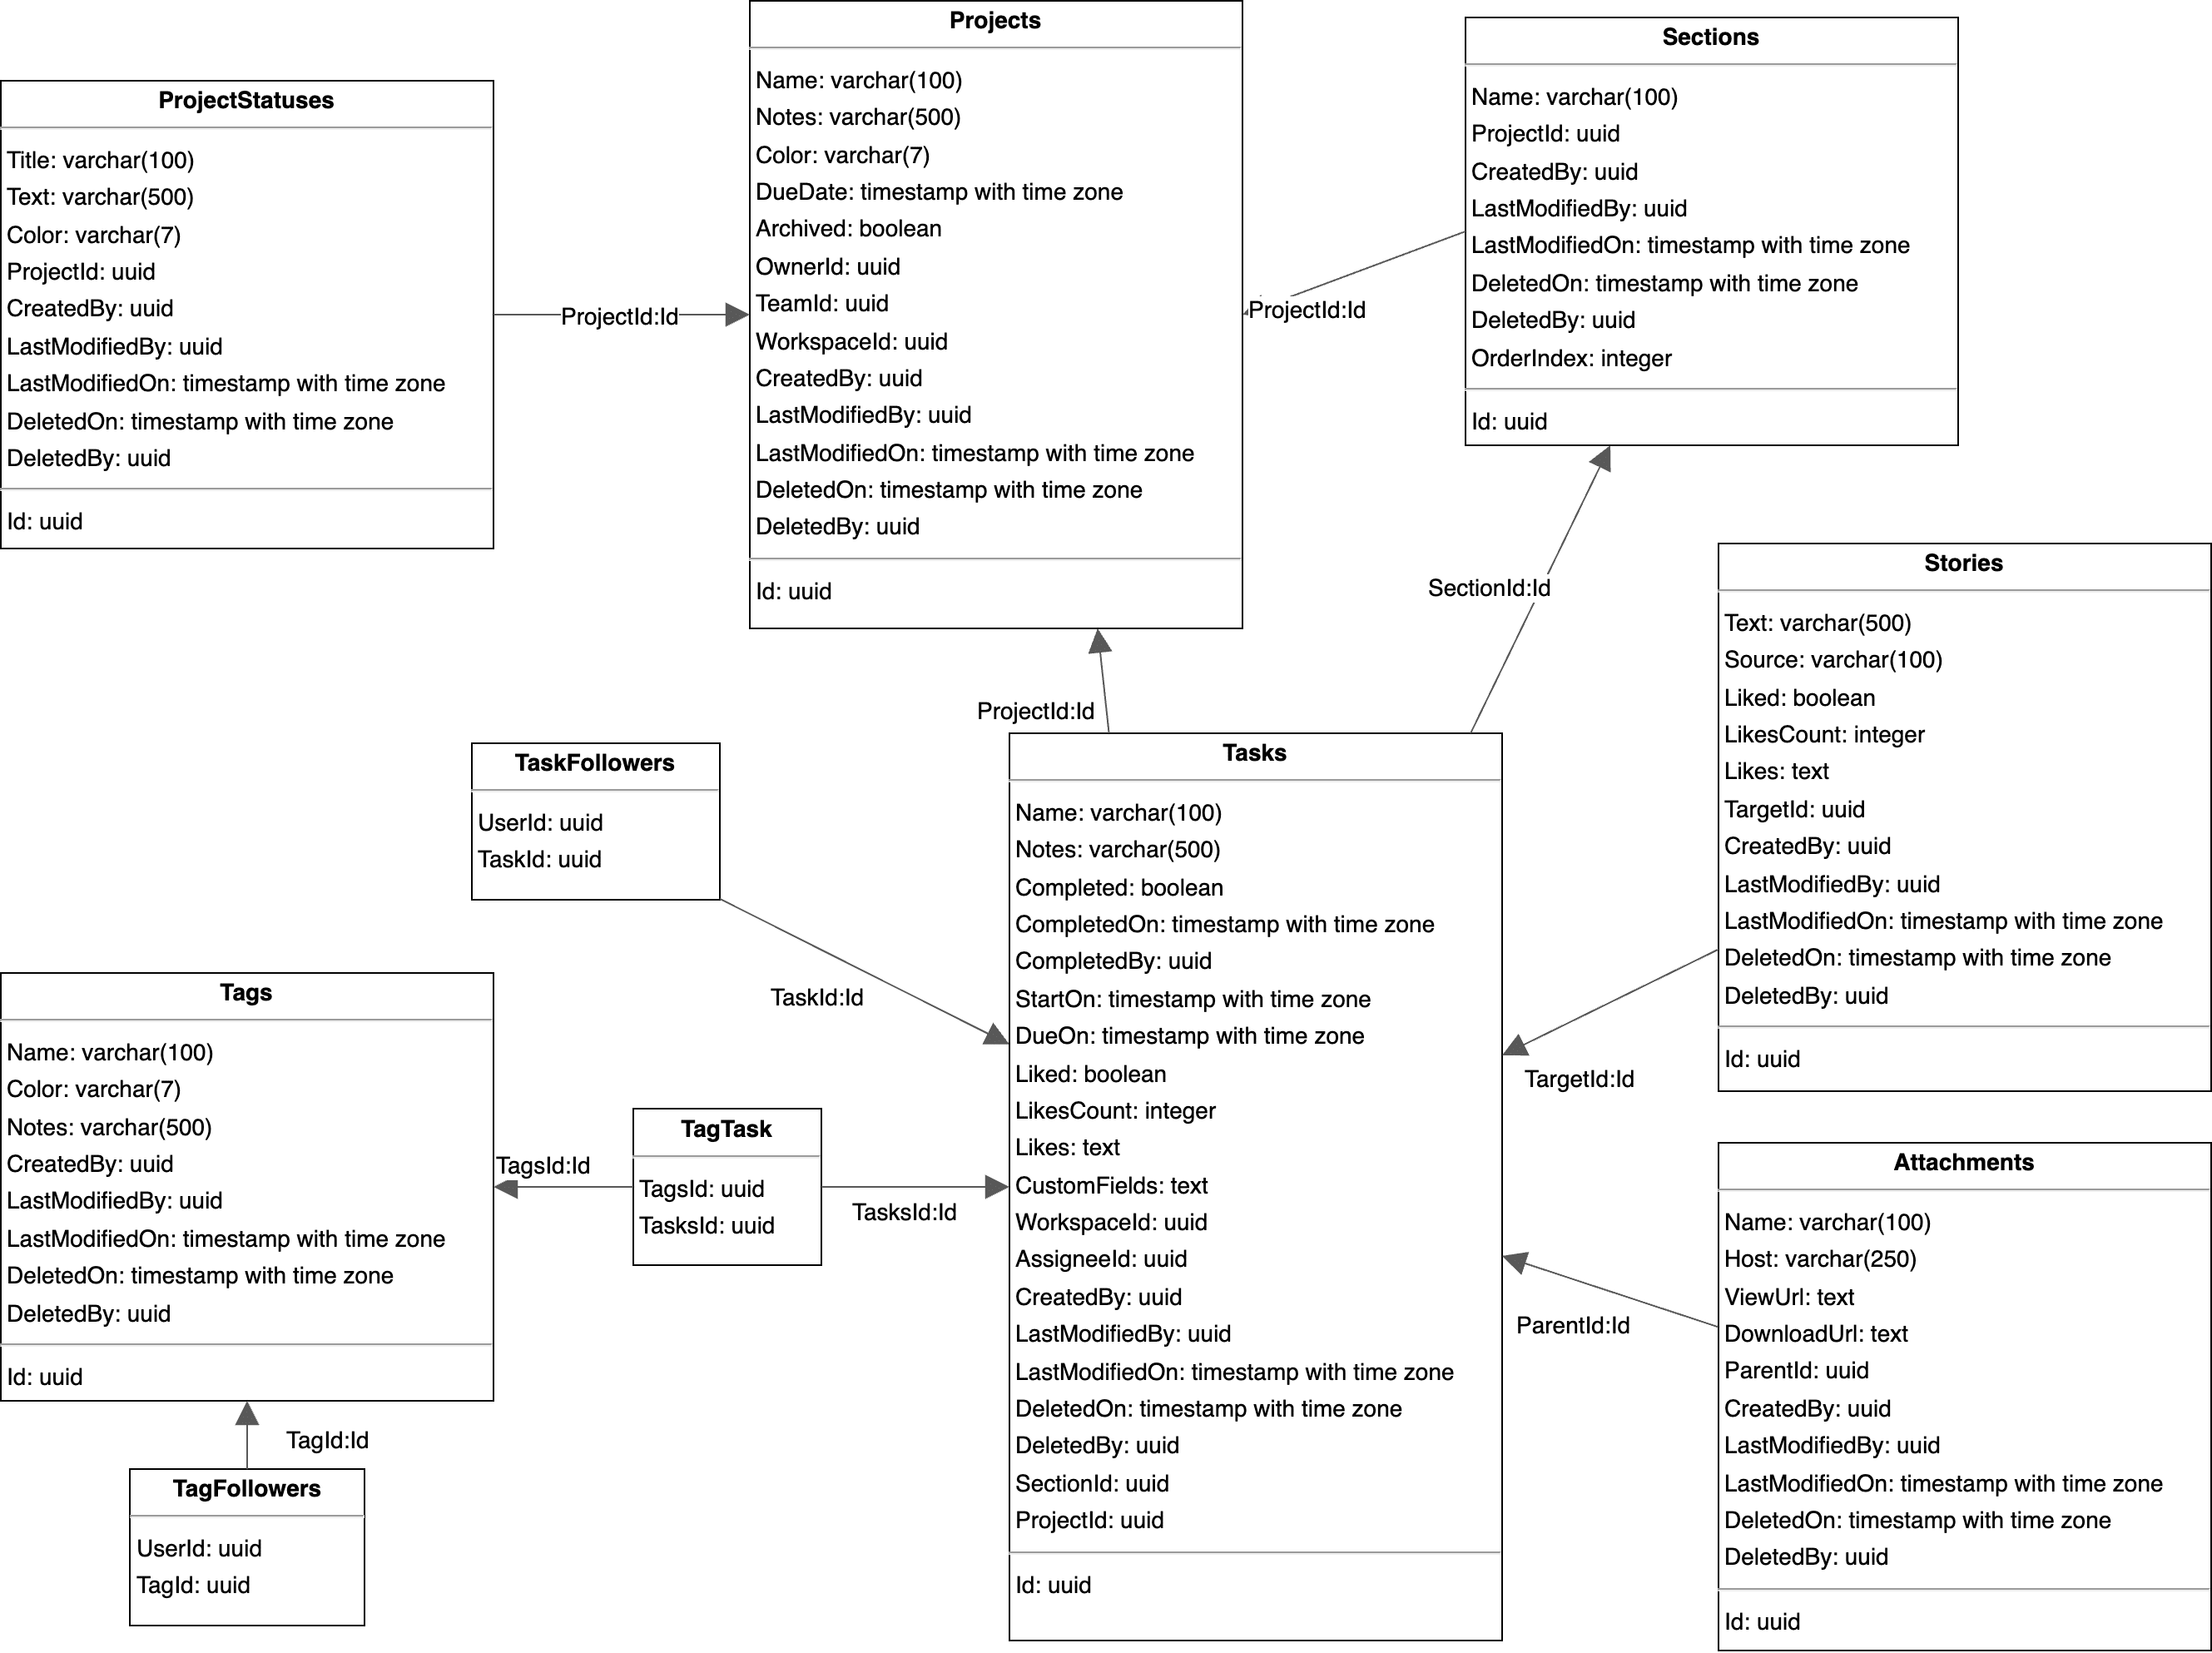
\includegraphics[width=1.1\linewidth]{Hinhve/PortalDbDiagram.png}
    \caption{Thiết kế cơ sở dữ liệu của dịch vụ Portal}
    \label{fig:PortalDbDiagram}
\end{figure}

Cơ sở dữ liệu của dịch vụ Personal được thiết kế gồm các bảng chính là People, Teams, Workspaces, và Organizationss. Các bảng này tương ứng với các thực thể
trong tầng ứng dụng của dịch vụ Personal. Các bảng còn lại là các bảng phụ, có tác dụng liên kết, bổ sung thông tin cho các bảng chính.

\begin{figure}[H]
    \centering
    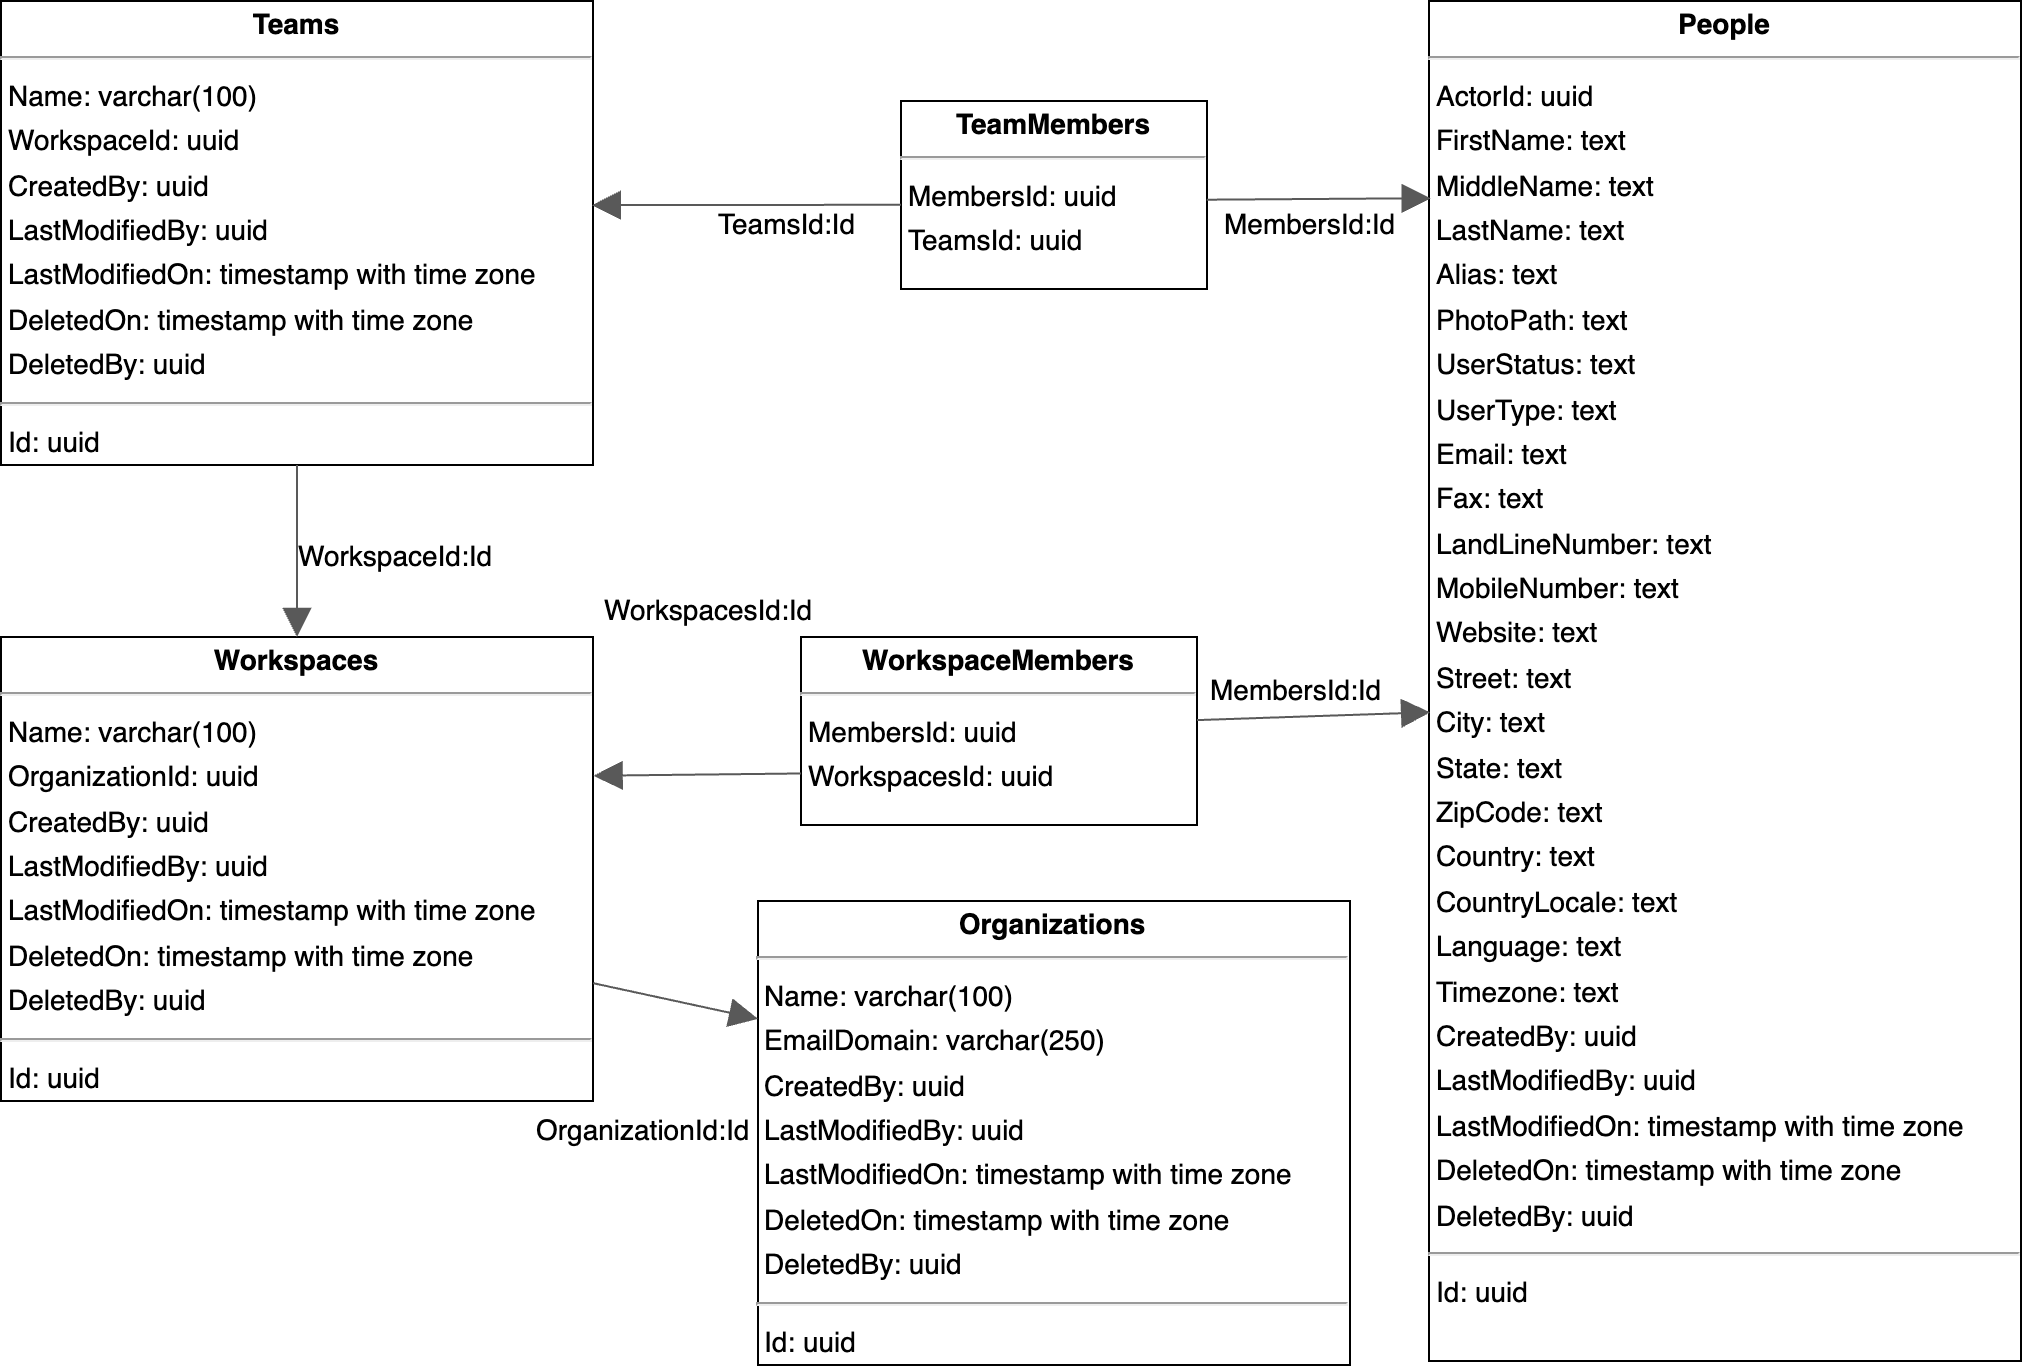
\includegraphics[width=1.1\linewidth]{Hinhve/PersonalDbDiagram.png}
    \caption{Thiết kế cơ sở dữ liệu của dịch vụ Personal}
    \label{fig:PersonalDbDiagram}
\end{figure}

\section{Xây dựng ứng dụng}
\label{section:4.3}
\subsection{Thư viện và công cụ sử dụng}
\label{subsection:4.3.1}

\begin{table}[H]
    \renewcommand{\arraystretch}{1.2}
    \centering{}
    \begin{tabular}{p{0.2\linewidth}p{0.3\linewidth}p{0.5\linewidth}}
        \hline
        \textbf{Mục đích}          & \textbf{Công cụ}          & \textbf{Địa chỉ URL}                            \\ \hline
        IDE lập trình              & Jetbrains Rider 2023.3    & https://www.jetbrains.com/rider/                \\ \hline
        IDE lập trình              & Jetbrains WebStorm 2023.3 & https://www.jetbrains.com/webstorm/             \\ \hline
        IDE lập trình              & Jetbrains DataGrip 2023.3 & https://www.jetbrains.com/datagrip/             \\ \hline
        IDE lập trình              & Visual Studio Code 1.85   & https://code.visualstudio.com/                  \\ \hline
        Công cụ kiểm thử API       & Postman 10.20             & https://www.postman.com/                        \\ \hline
        Công cụ quản lý mã nguồn   & Git Kraken 9.10.0         & https://www.gitkraken.com/                      \\ \hline
        Công cụ quản lý container  & Docker Desktop 4.25.2     & https://www.docker.com/products/docker-desktop/ \\ \hline
        Công cụ quản lý Kubernetes & Lens 2023.12              & https://k8slens.dev/                            \\ \hline
    \end{tabular}
    \renewcommand{\arraystretch}{1}
    \caption{Danh sách thư viện và công cụ sử dụng}
    \label{fig:libaries_and_tools}
\end{table}

\newpage

\subsection{Kết quả đạt được}
\label{subsection:4.3.2}

Sau quá trình thực hiện đồ án, em đã xây dựng thành công một hệ thống quản lý dự án dựa trên kiến trúc Microservices theo yêu cầu đồ án
đã trình bày ở Chương 2. Sản phẩm đầu ra bao gồm một hệ thống back-end và một ứng dụng front-end, được triển khai trên môi trường đám mây.
Trong đó, hệ thống back-end bao gồm các dịch vụ khác nhau được triển khai trên một cụm Kubernetes được quản lý bởi Google Kubernetes Engine.
Chúng cung cấp các API để giao tiếp với ứng dụng front-end, cũng như với các dịch vụ khác trong hệ thống. Ngoài ra, hệ thống này còn triển khai một
máy chủ xác thực riêng và độc lập với các dịch vụ khác.
Về ứng dụng front-end, no được triển khai trên trên một máy chủ riêng nhằm đảm bảo tốc độ phản hồi tốt nhất cho người dùng.

Về mã nguồn, em cũng chia chúng làm hai phần tương ứng với hệ thống back-end và ứng dụng front-end.
Mã nguồn của cả được lưu trữ trên GitHub, trong đó có bao gồm các tệp tin cấu hình để triển khai trên môi trường đám mây, cấu hình
tài nguyên cho các dịch vụ, hướng dẫn triển khai và vận hành hệ thống.

Dưới đây, em xin thống kê lại các thông số khác về đồ án mà em đã thực hiện.

\begin{table}[H]
    \renewcommand{\arraystretch}{1.2}
    \centering{}
    \begin{tabular}{p{0.7\linewidth}p{0.3\linewidth}}
        \hline
        Số lượng dòng code trong mã nguồn & TBC \\ \hline
        Số lượng lớp trong mã nguồn       & TBC \\ \hline
        Số lượng gói trong mã nguồn       & TBC \\ \hline
        Dung lượng mã nguồn               & TBC \\ \hline
        Số lượng bảng trong cơ sở dữ liệu & TBC \\ \hline
        Dung lượng cơ sở dữ liệu          & TBC \\ \hline
        Tổng thời gian thực hiện mã nguồn & TBC \\ \hline
    \end{tabular}
    \renewcommand{\arraystretch}{1}
    \caption{Thống kê các thông số về đồ án}
    \label{fig:project_statistics}
\end{table}

\newpage


\subsection{Minh họa các chức năng chính}
\label{subsection:4.3.3}

\begin{figure}[H]
    \centering
    \includegraphics[width=1.0\linewidth]{Hinhve/Screenshot_Landing.png}
    \caption{Minh hoạ giao diện Trang chủ}
    \label{fig:Screenshot_Landing}
\end{figure}


\begin{figure}[H]
    \centering
    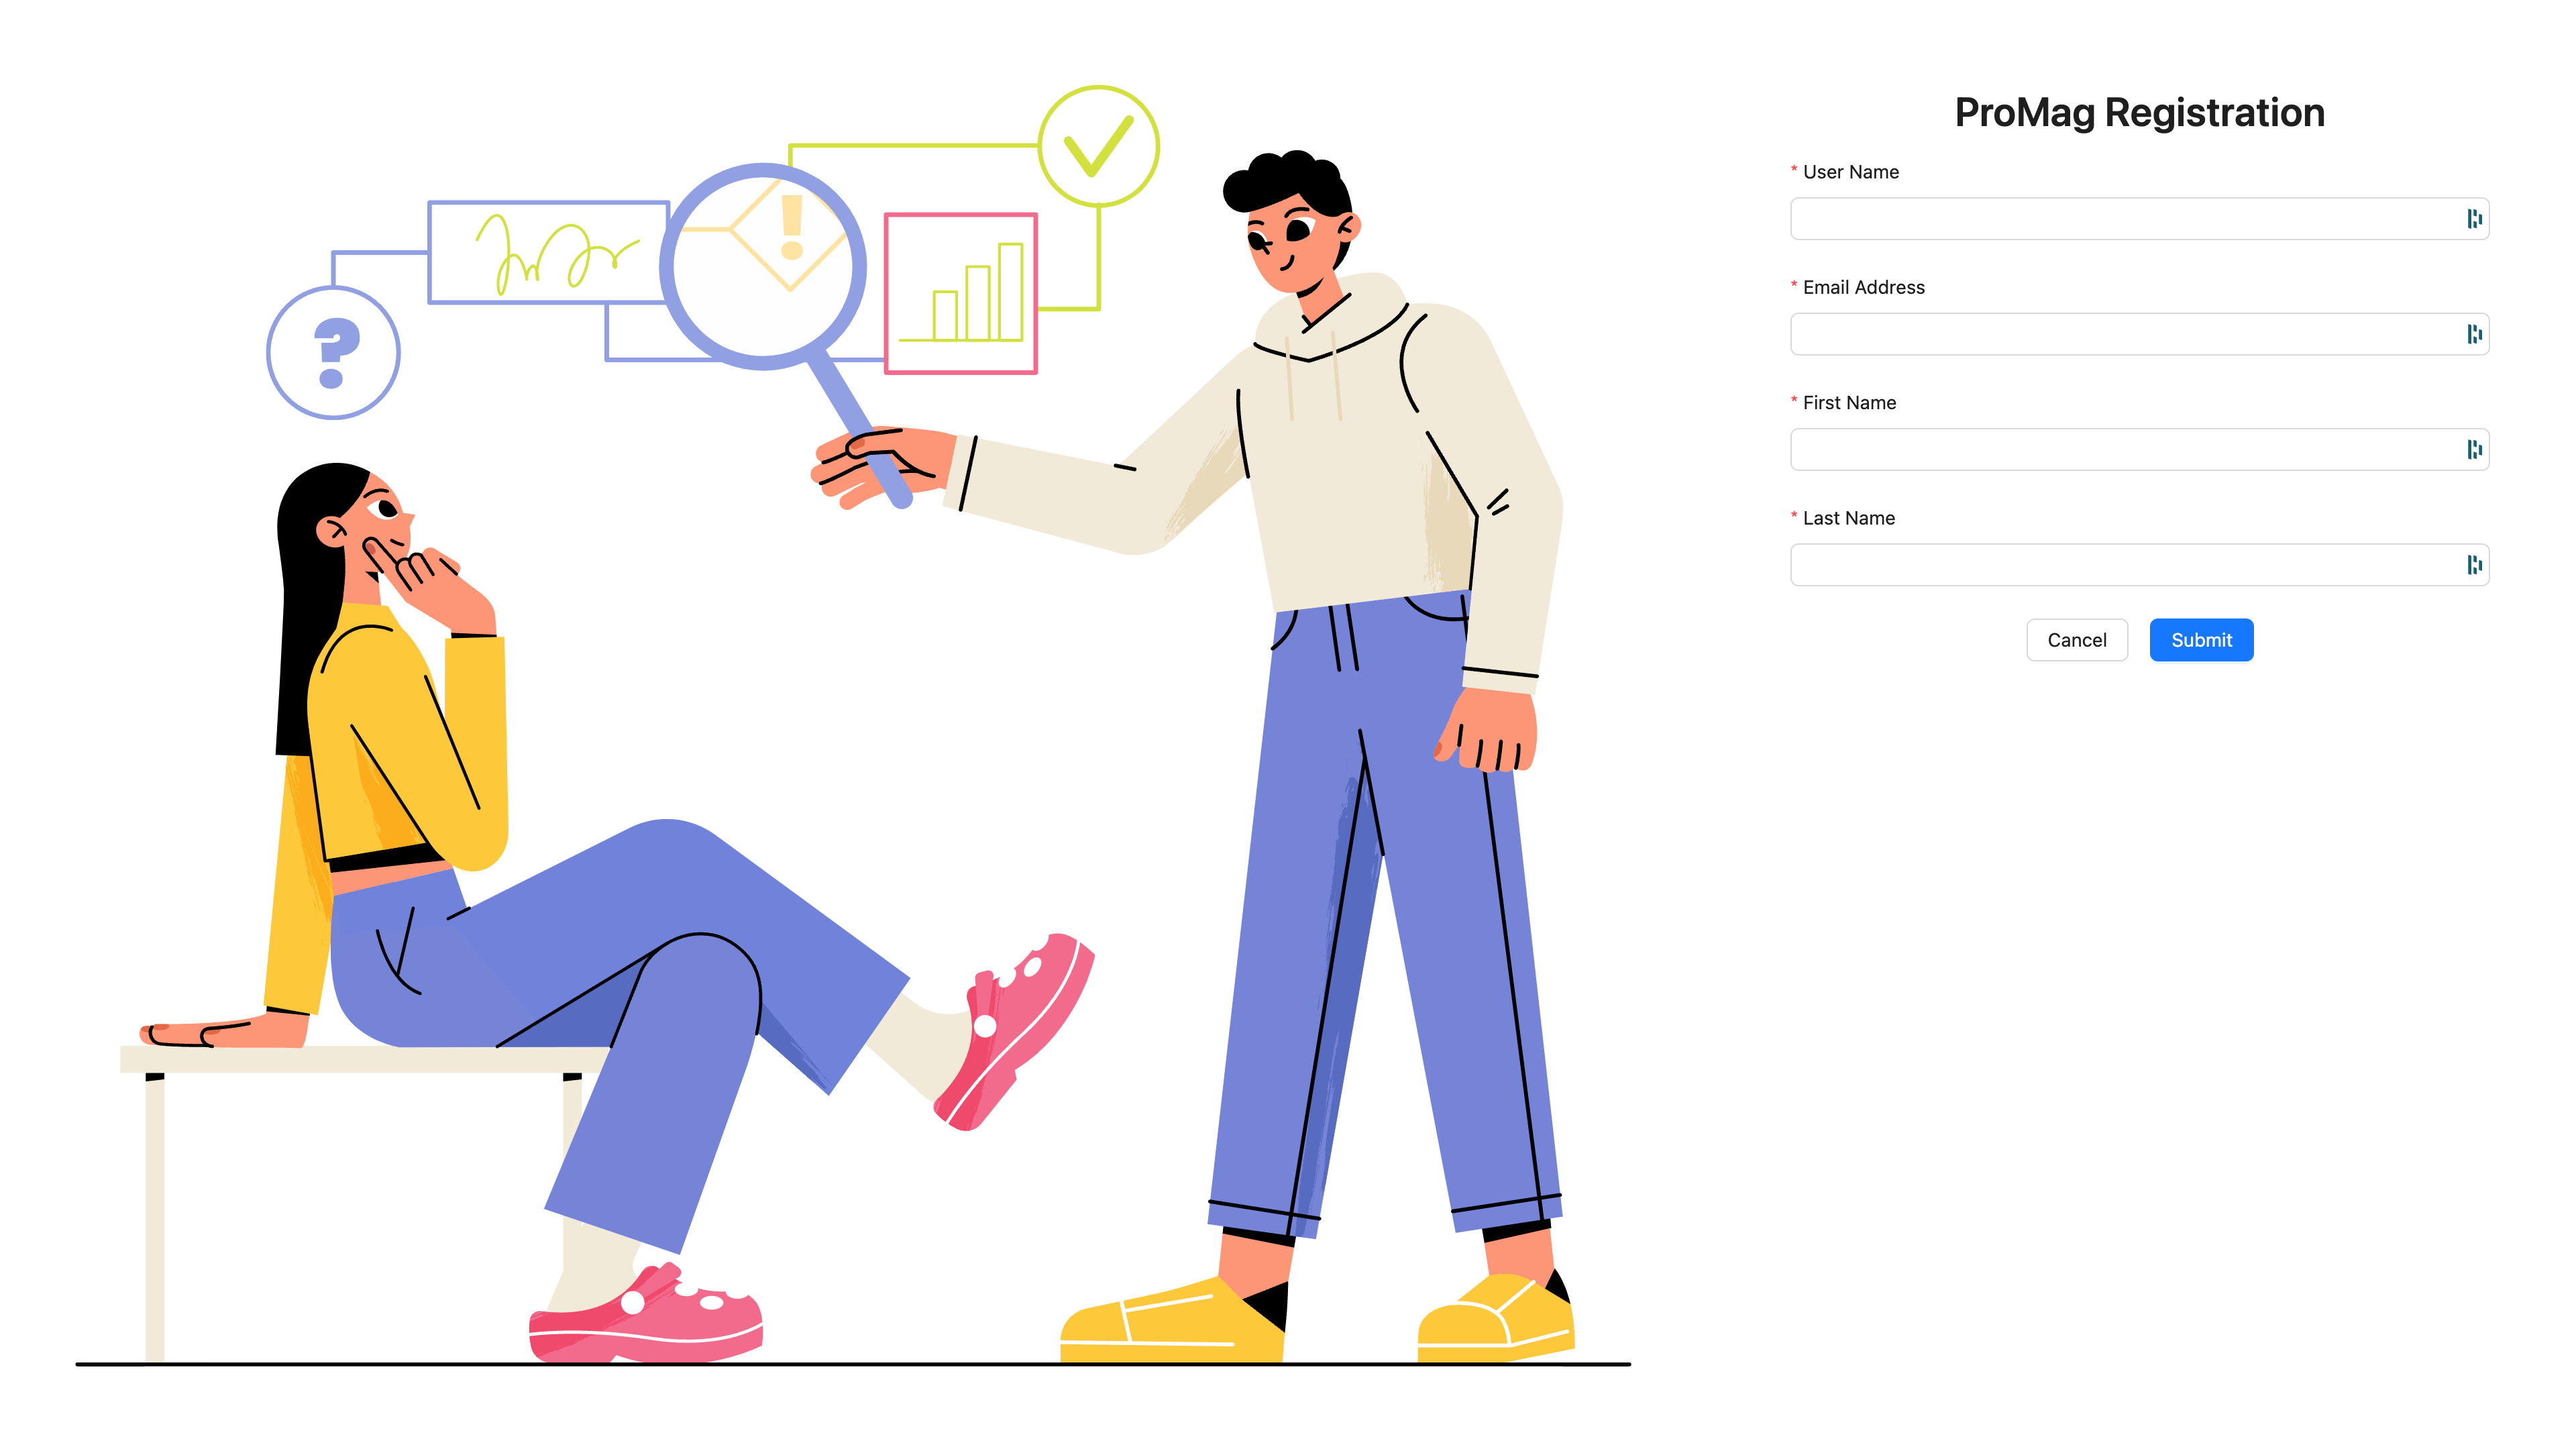
\includegraphics[width=1.0\linewidth]{Hinhve/Screenshot_Register.png}
    \caption{Minh hoạ giao diện Đăng ký}
    \label{fig:Screenshot_Register}
\end{figure}

\newpage

\begin{figure}[H]
    \centering
    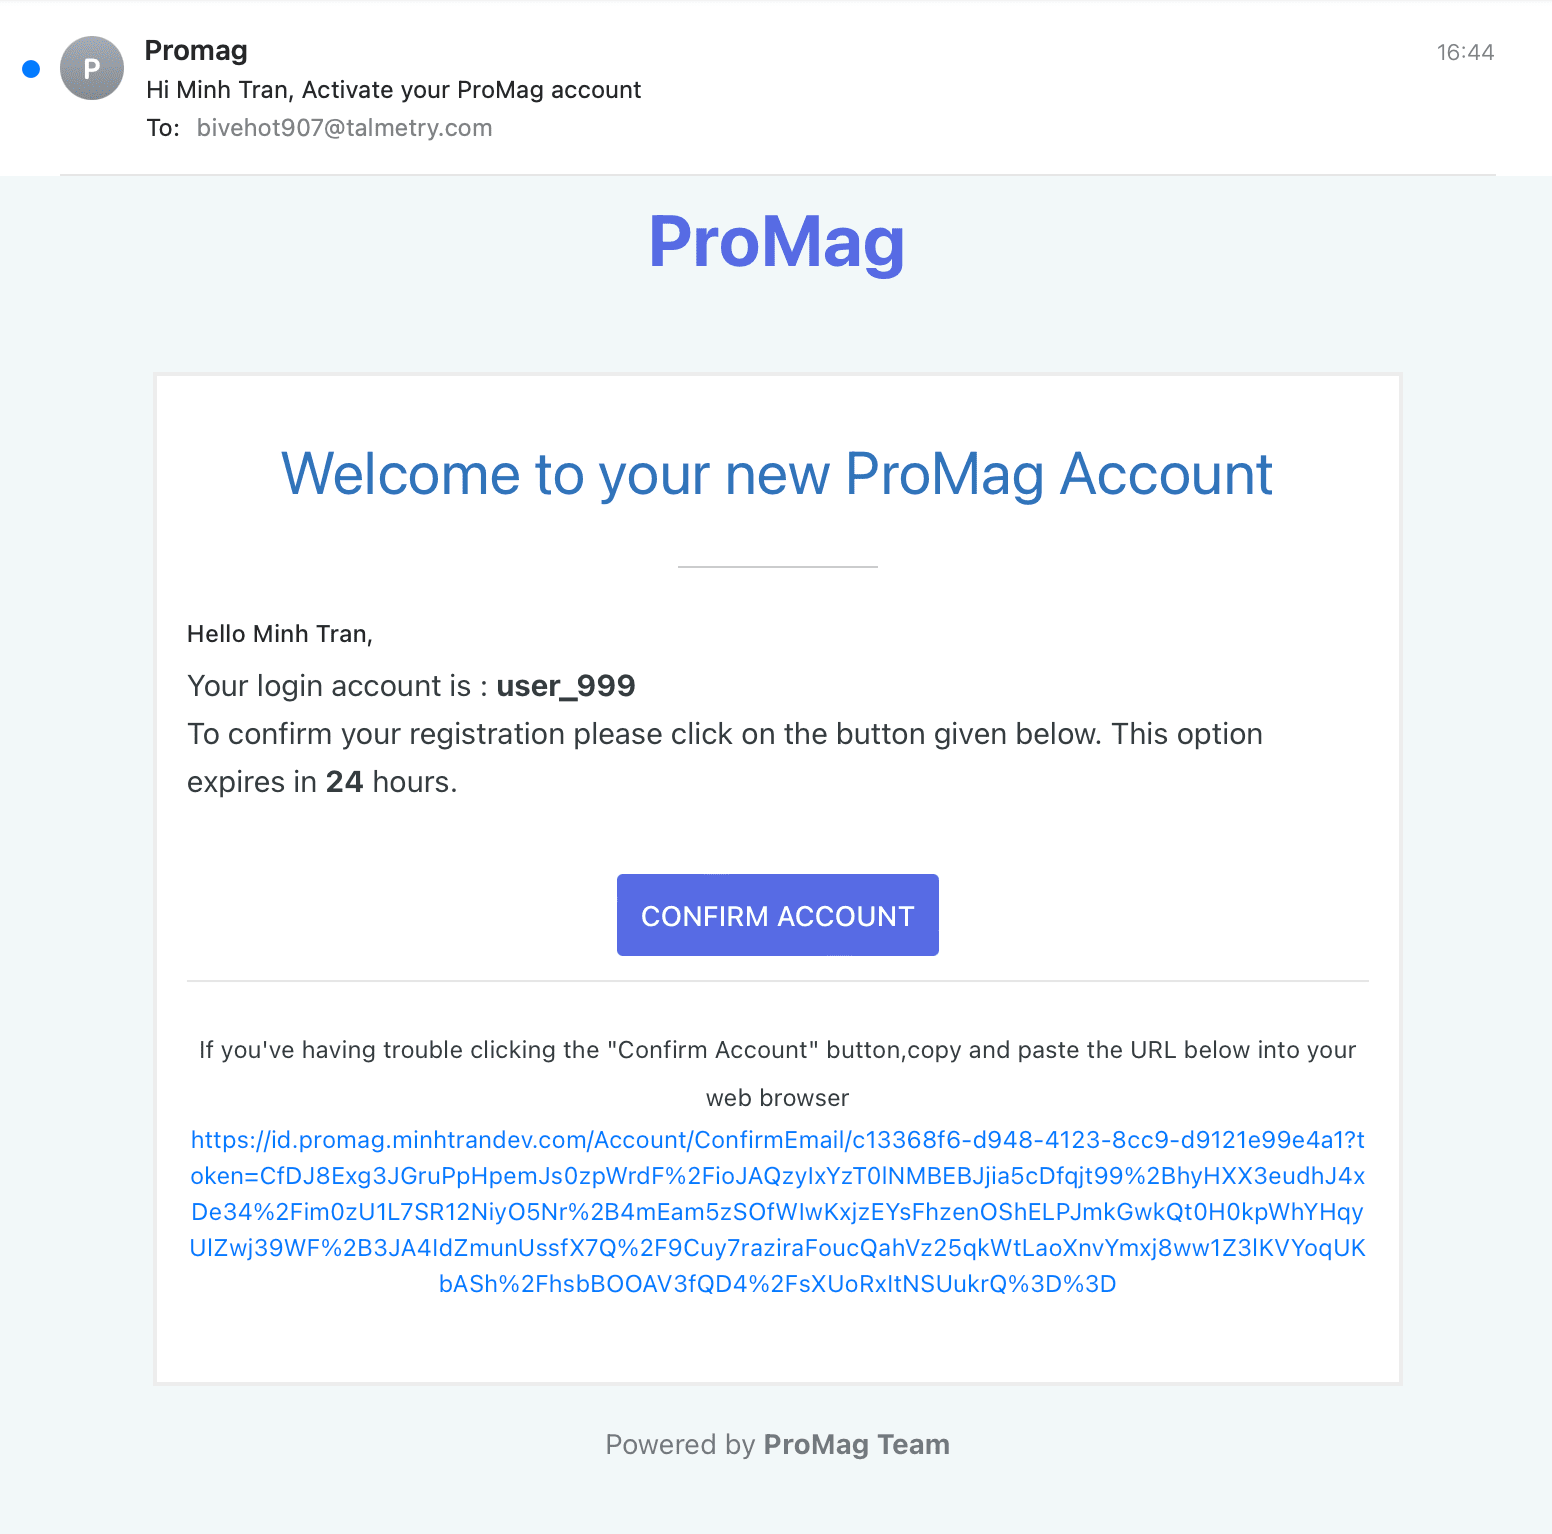
\includegraphics[width=1.0\linewidth]{Hinhve/Screenshot_CreateAccountEmail.png}
    \caption{Minh hoạ giao diện Thư điện tử xác nhận tài khoản}
    \label{fig:Screenshot_CreateAccountEmail}
\end{figure}

\newpage

\begin{figure}[H]
    \centering
    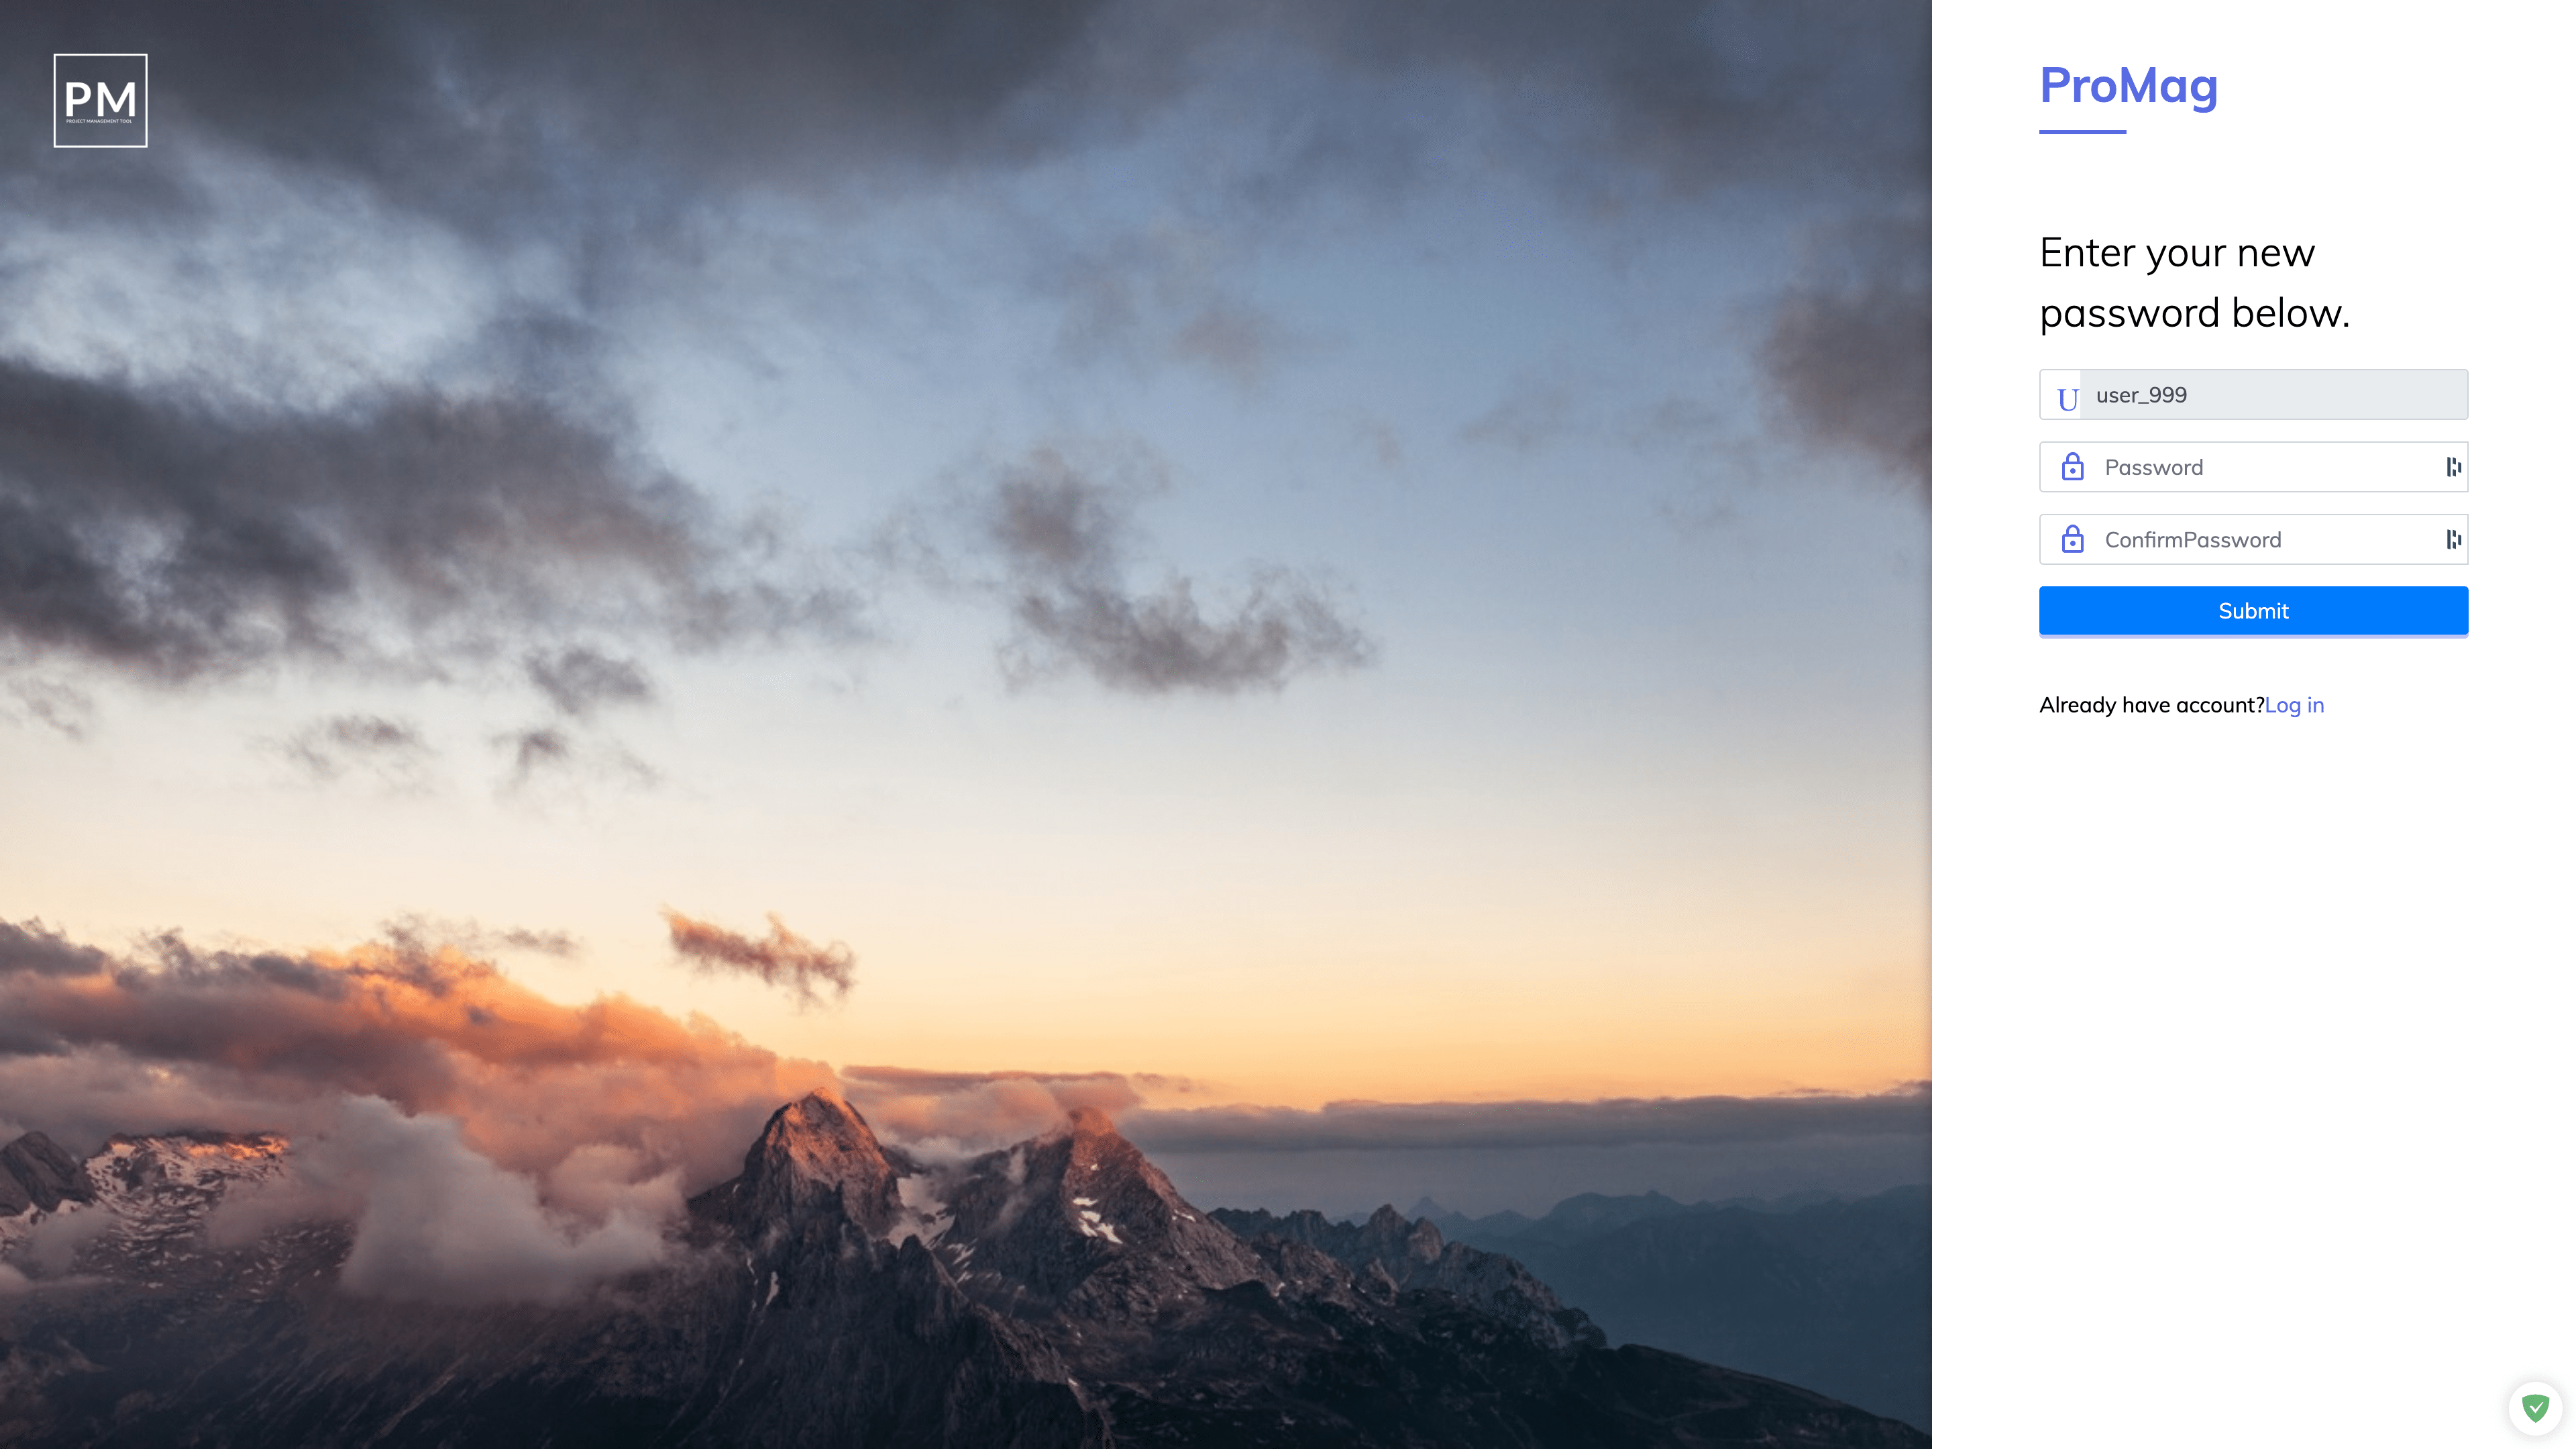
\includegraphics[width=1.0\linewidth]{Hinhve/Screenshot_CreatePassword.png}
    \caption{Minh hoạ giao diện Tạo mật khẩu}
    \label{fig:Screenshot_CreatePassword}
\end{figure}


\begin{figure}[H]
    \centering
    \includegraphics[width=1.0\linewidth]{Hinhve/Screenshot_CreatePasswordSuccess.png}
    \caption{Minh hoạ giao diện Tạo mật khẩu thành công}
    \label{fig:Screenshot_CreatePasswordSuccess}
\end{figure}

\newpage

\begin{figure}[H]
    \centering
    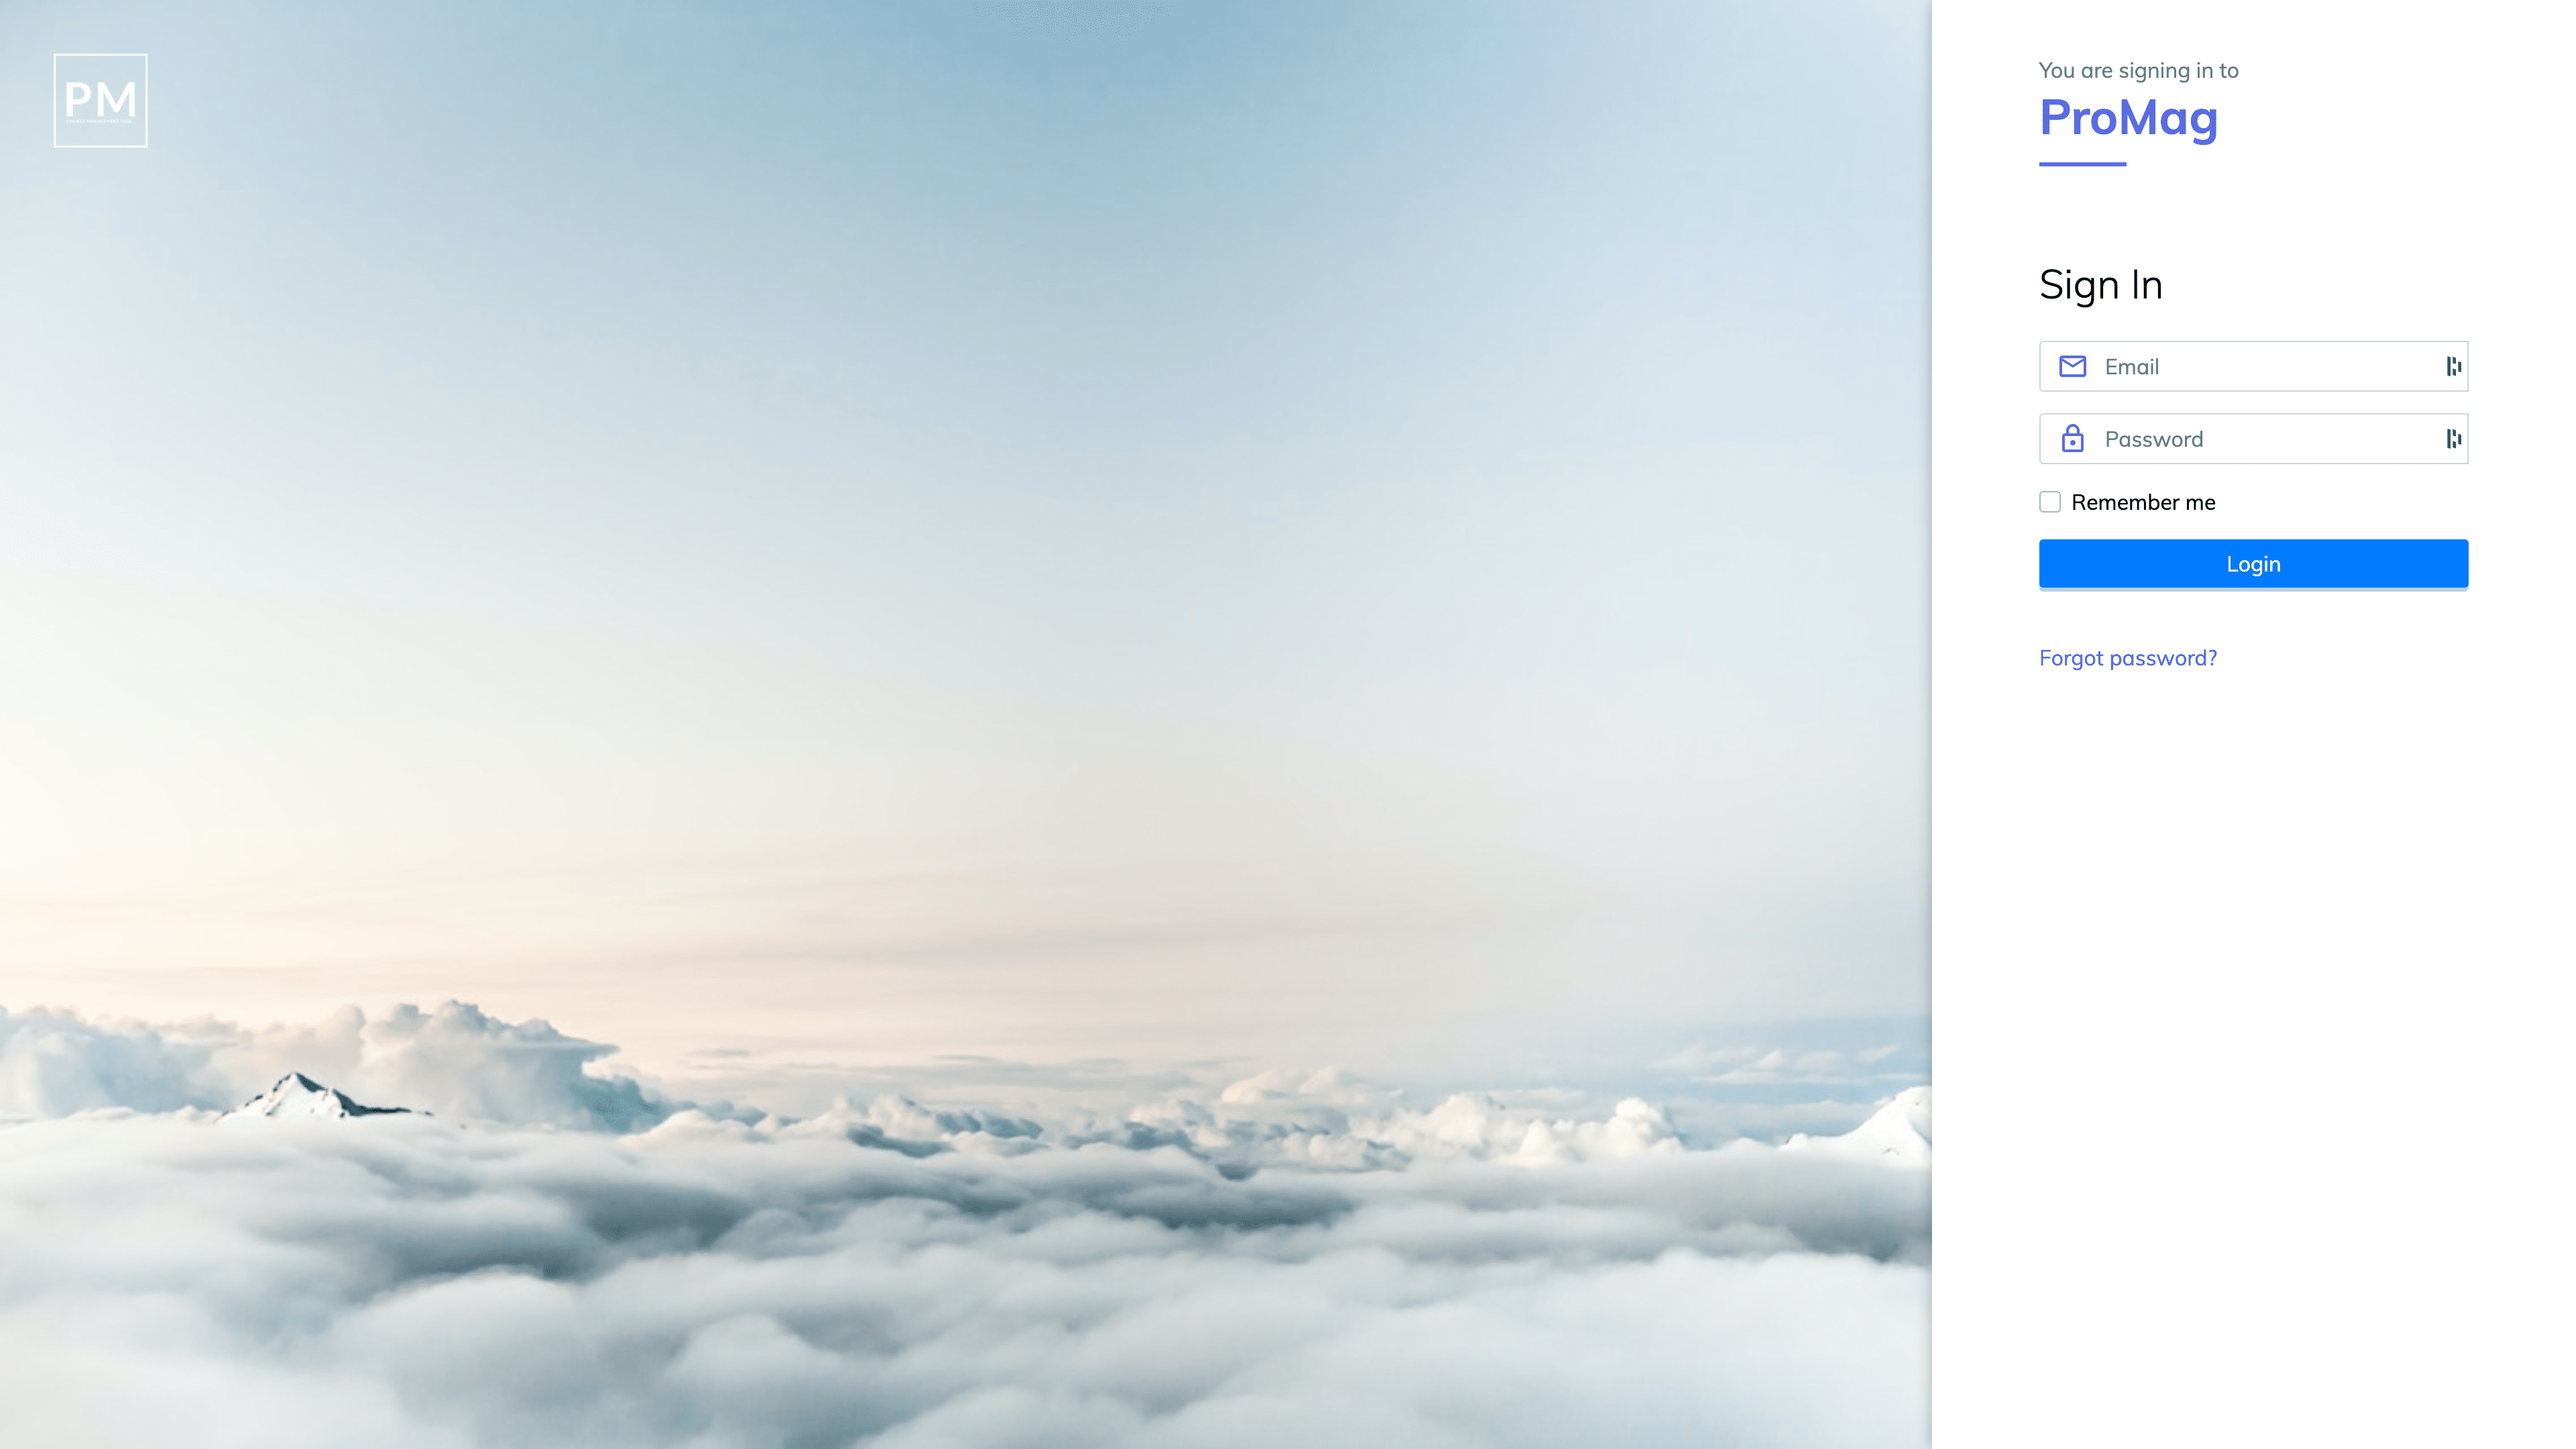
\includegraphics[width=1.0\linewidth]{Hinhve/Screenshot_Login.png}
    \caption{Minh hoạ giao diện Đăng nhập}
    \label{fig:Screenshot_Login}
\end{figure}


\begin{figure}[H]
    \centering
    \includegraphics[width=1.0\linewidth]{Hinhve/Screenshot_LoginSuccess.png}
    \caption{Minh hoạ giao diện Đăng nhập thành công}
    \label{fig:Screenshot_LoginSuccess}
\end{figure}

\newpage

\begin{figure}[H]
    \centering
    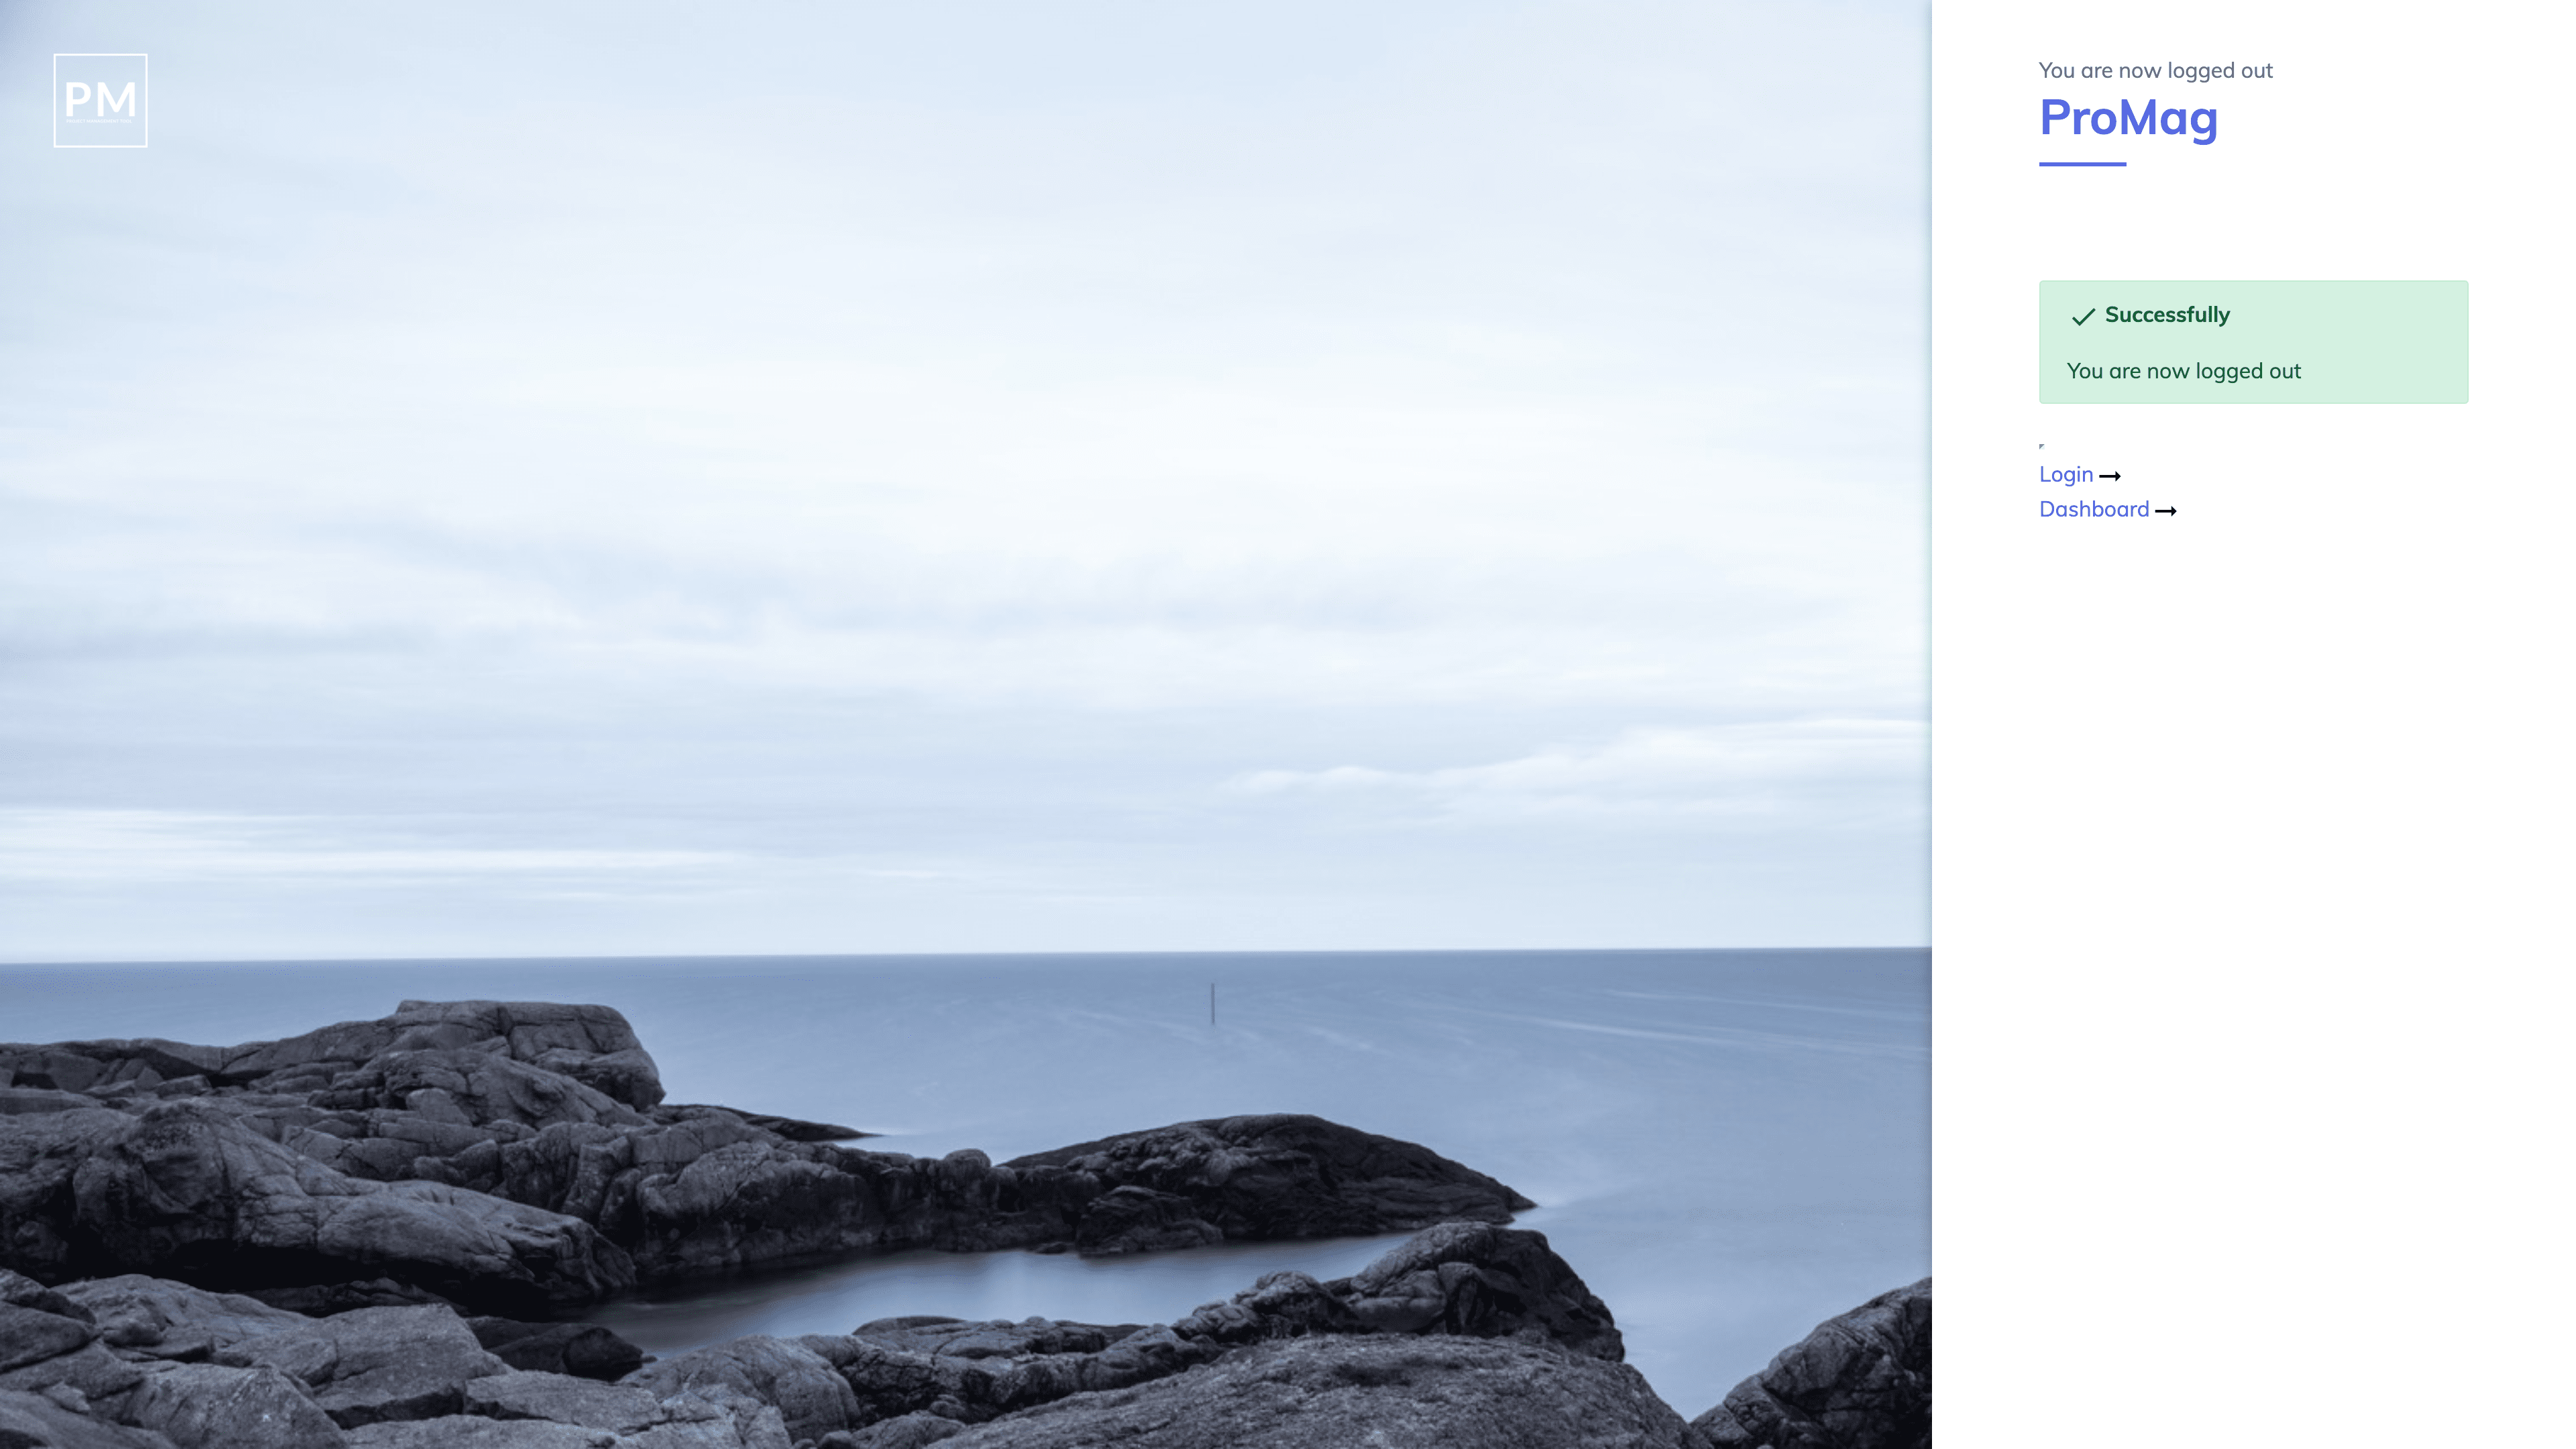
\includegraphics[width=1.0\linewidth]{Hinhve/Screenshot_LogoutSuccess.png}
    \caption{Minh hoạ giao diện Đăng xuất thành công}
    \label{fig:Screenshot_LogoutSuccess}
\end{figure}


\begin{figure}[H]
    \centering
    \includegraphics[width=1.0\linewidth]{Hinhve/Screenshot_ForgetPassword.png}
    \caption{Minh hoạ giao diện Quên mật khẩu}
    \label{fig:Screenshot_ForgetPassword}
\end{figure}

\newpage

\begin{figure}[H]
    \centering
    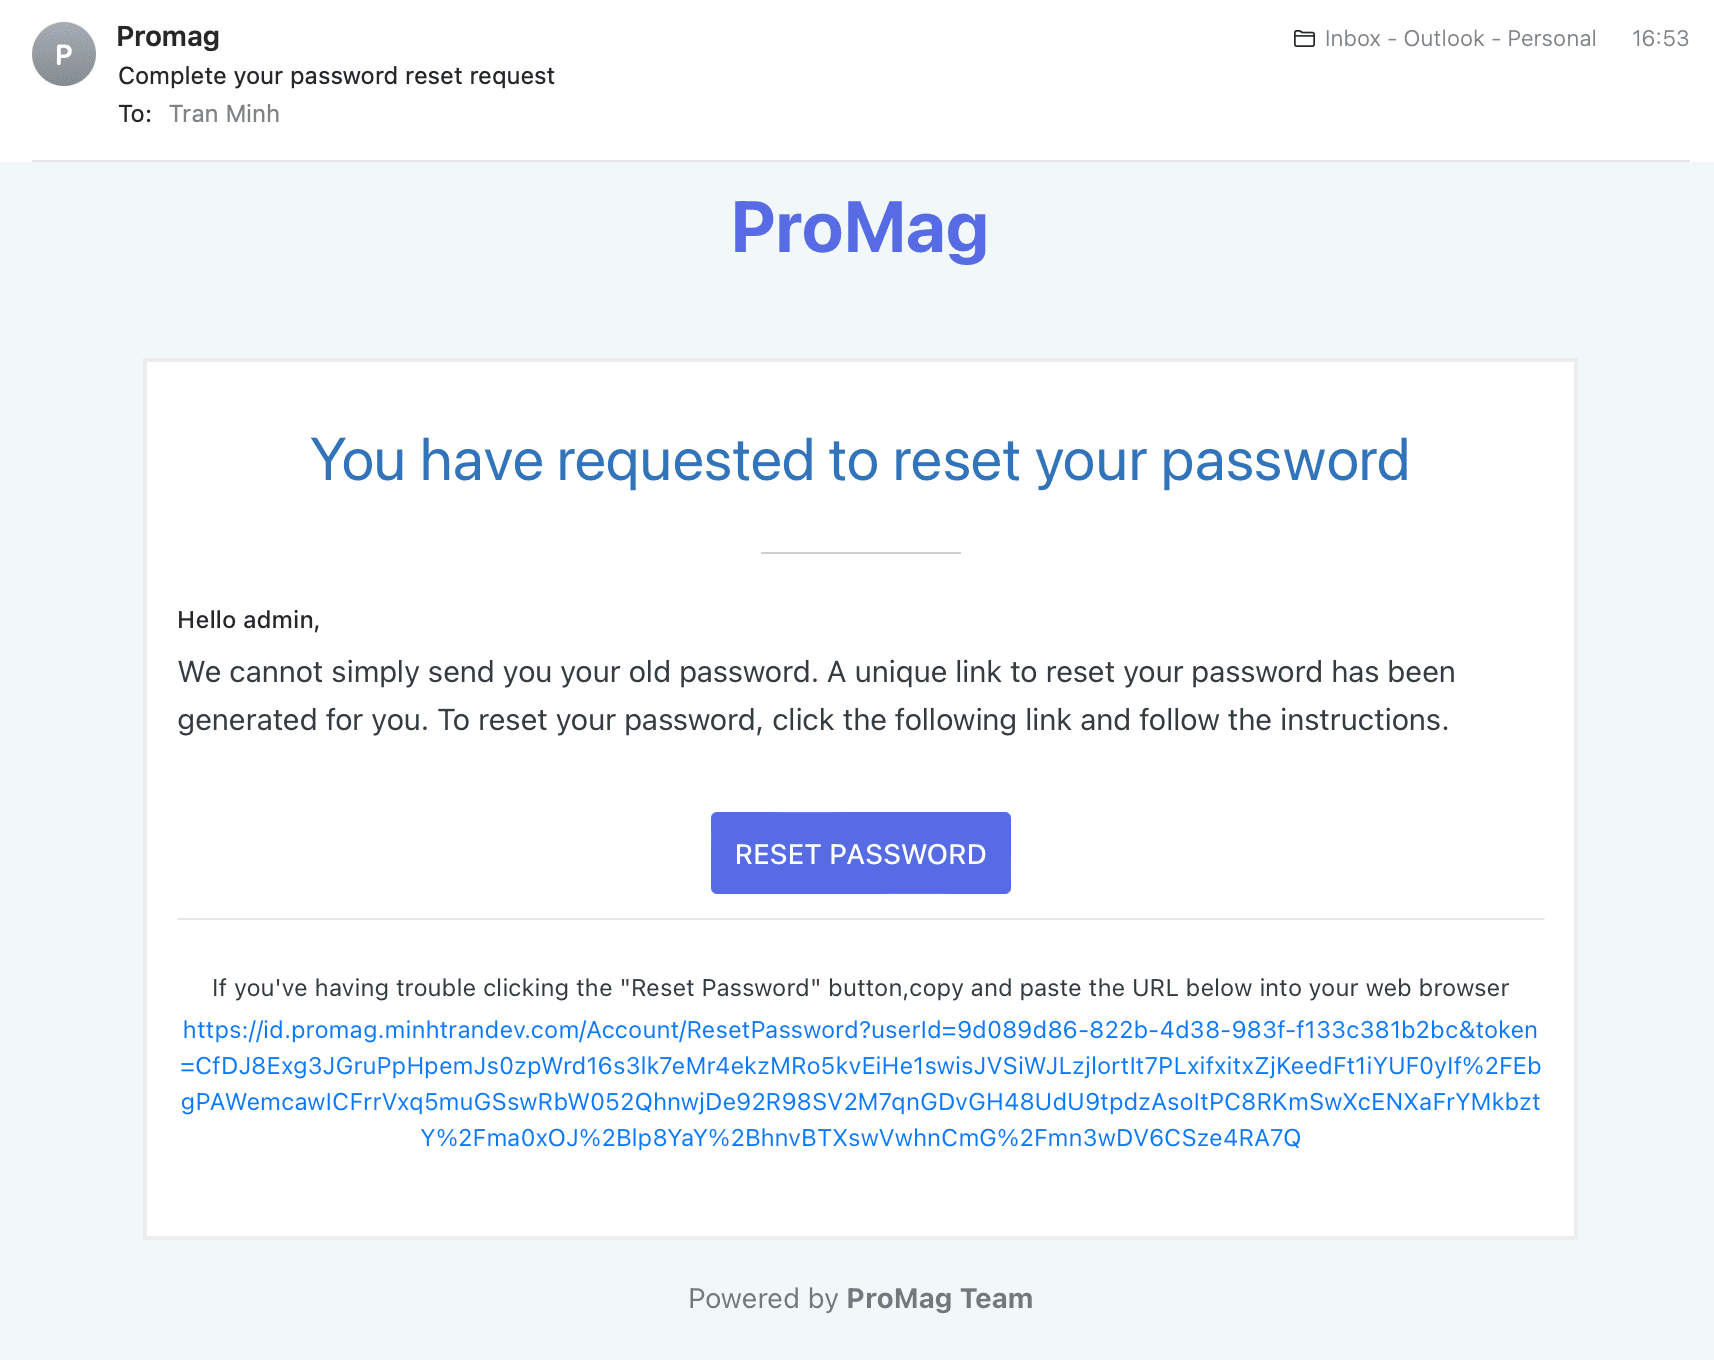
\includegraphics[width=1.0\linewidth]{Hinhve/Screenshot_ResetPasswordEmail.png}
    \caption{Minh hoạ giao diện Thư điện tử thiết lập lại mật khẩu}
    \label{fig:Screenshot_ResetPasswordEmail}
\end{figure}

\newpage

\begin{figure}[H]
    \centering
    \includegraphics[width=1.0\linewidth]{Hinhve/Screenshot_ResetPassword.png}
    \caption{Minh hoạ giao diện Thiết lập lại mật khẩu}
    \label{fig:Screenshot_ResetPassword}
\end{figure}

\begin{figure}[H]
    \centering
    \includegraphics[width=1.0\linewidth]{Hinhve/Screenshot_ResetPasswordSuccess.png}
    \caption{Minh hoạ giao diện Thiết lập lại mật khẩu thành công}
    \label{fig:Screenshot_ResetPasswordSuccess}
\end{figure}

\newpage

\begin{figure}[H]
    \centering
    \includegraphics[width=1.0\linewidth]{Hinhve/Screenshot_AcceptAccess.png}
    \caption{Minh hoạ giao diện Cấp quyền cho ứng dụng}
    \label{fig:Screenshot_AcceptAccess}
\end{figure}


\begin{figure}[H]
    \centering
    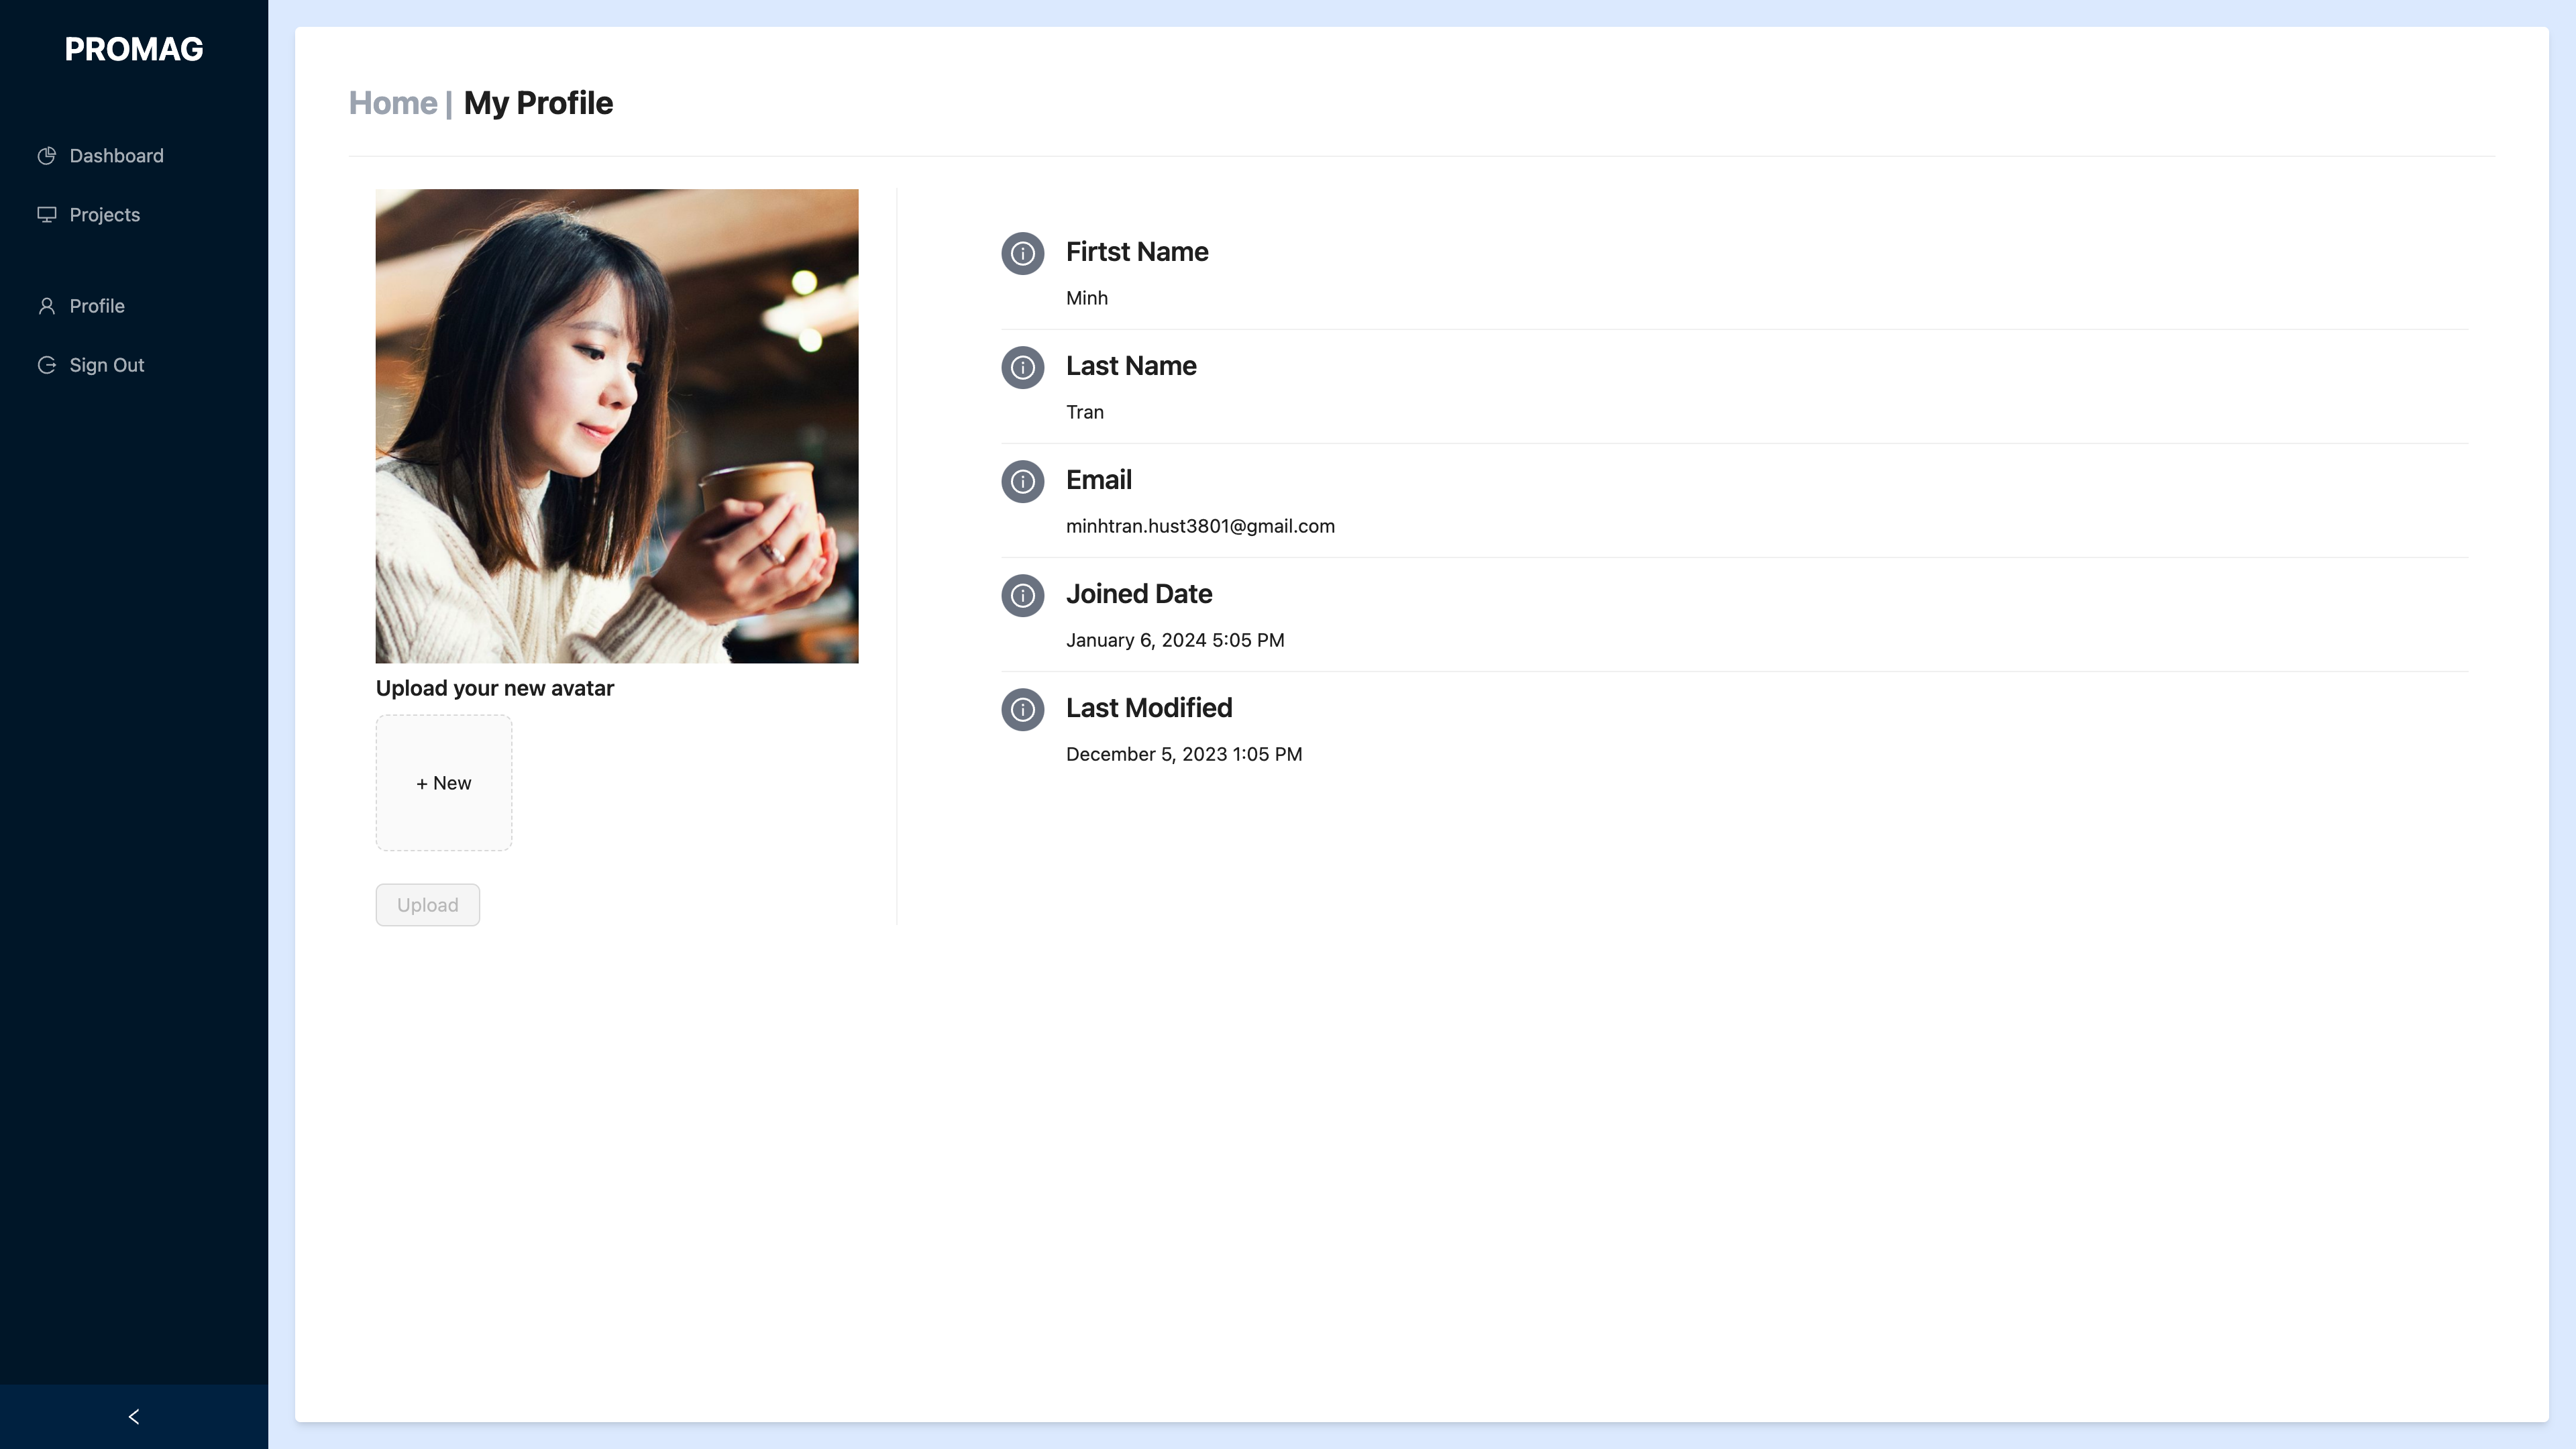
\includegraphics[width=1.0\linewidth]{Hinhve/Screenshot_MyProfile.png}
    \caption{Minh hoạ giao diện Hồ sơ của tôi}
    \label{fig:Screenshot_MyProfile}
\end{figure}

\newpage

\begin{figure}[H]
    \centering
    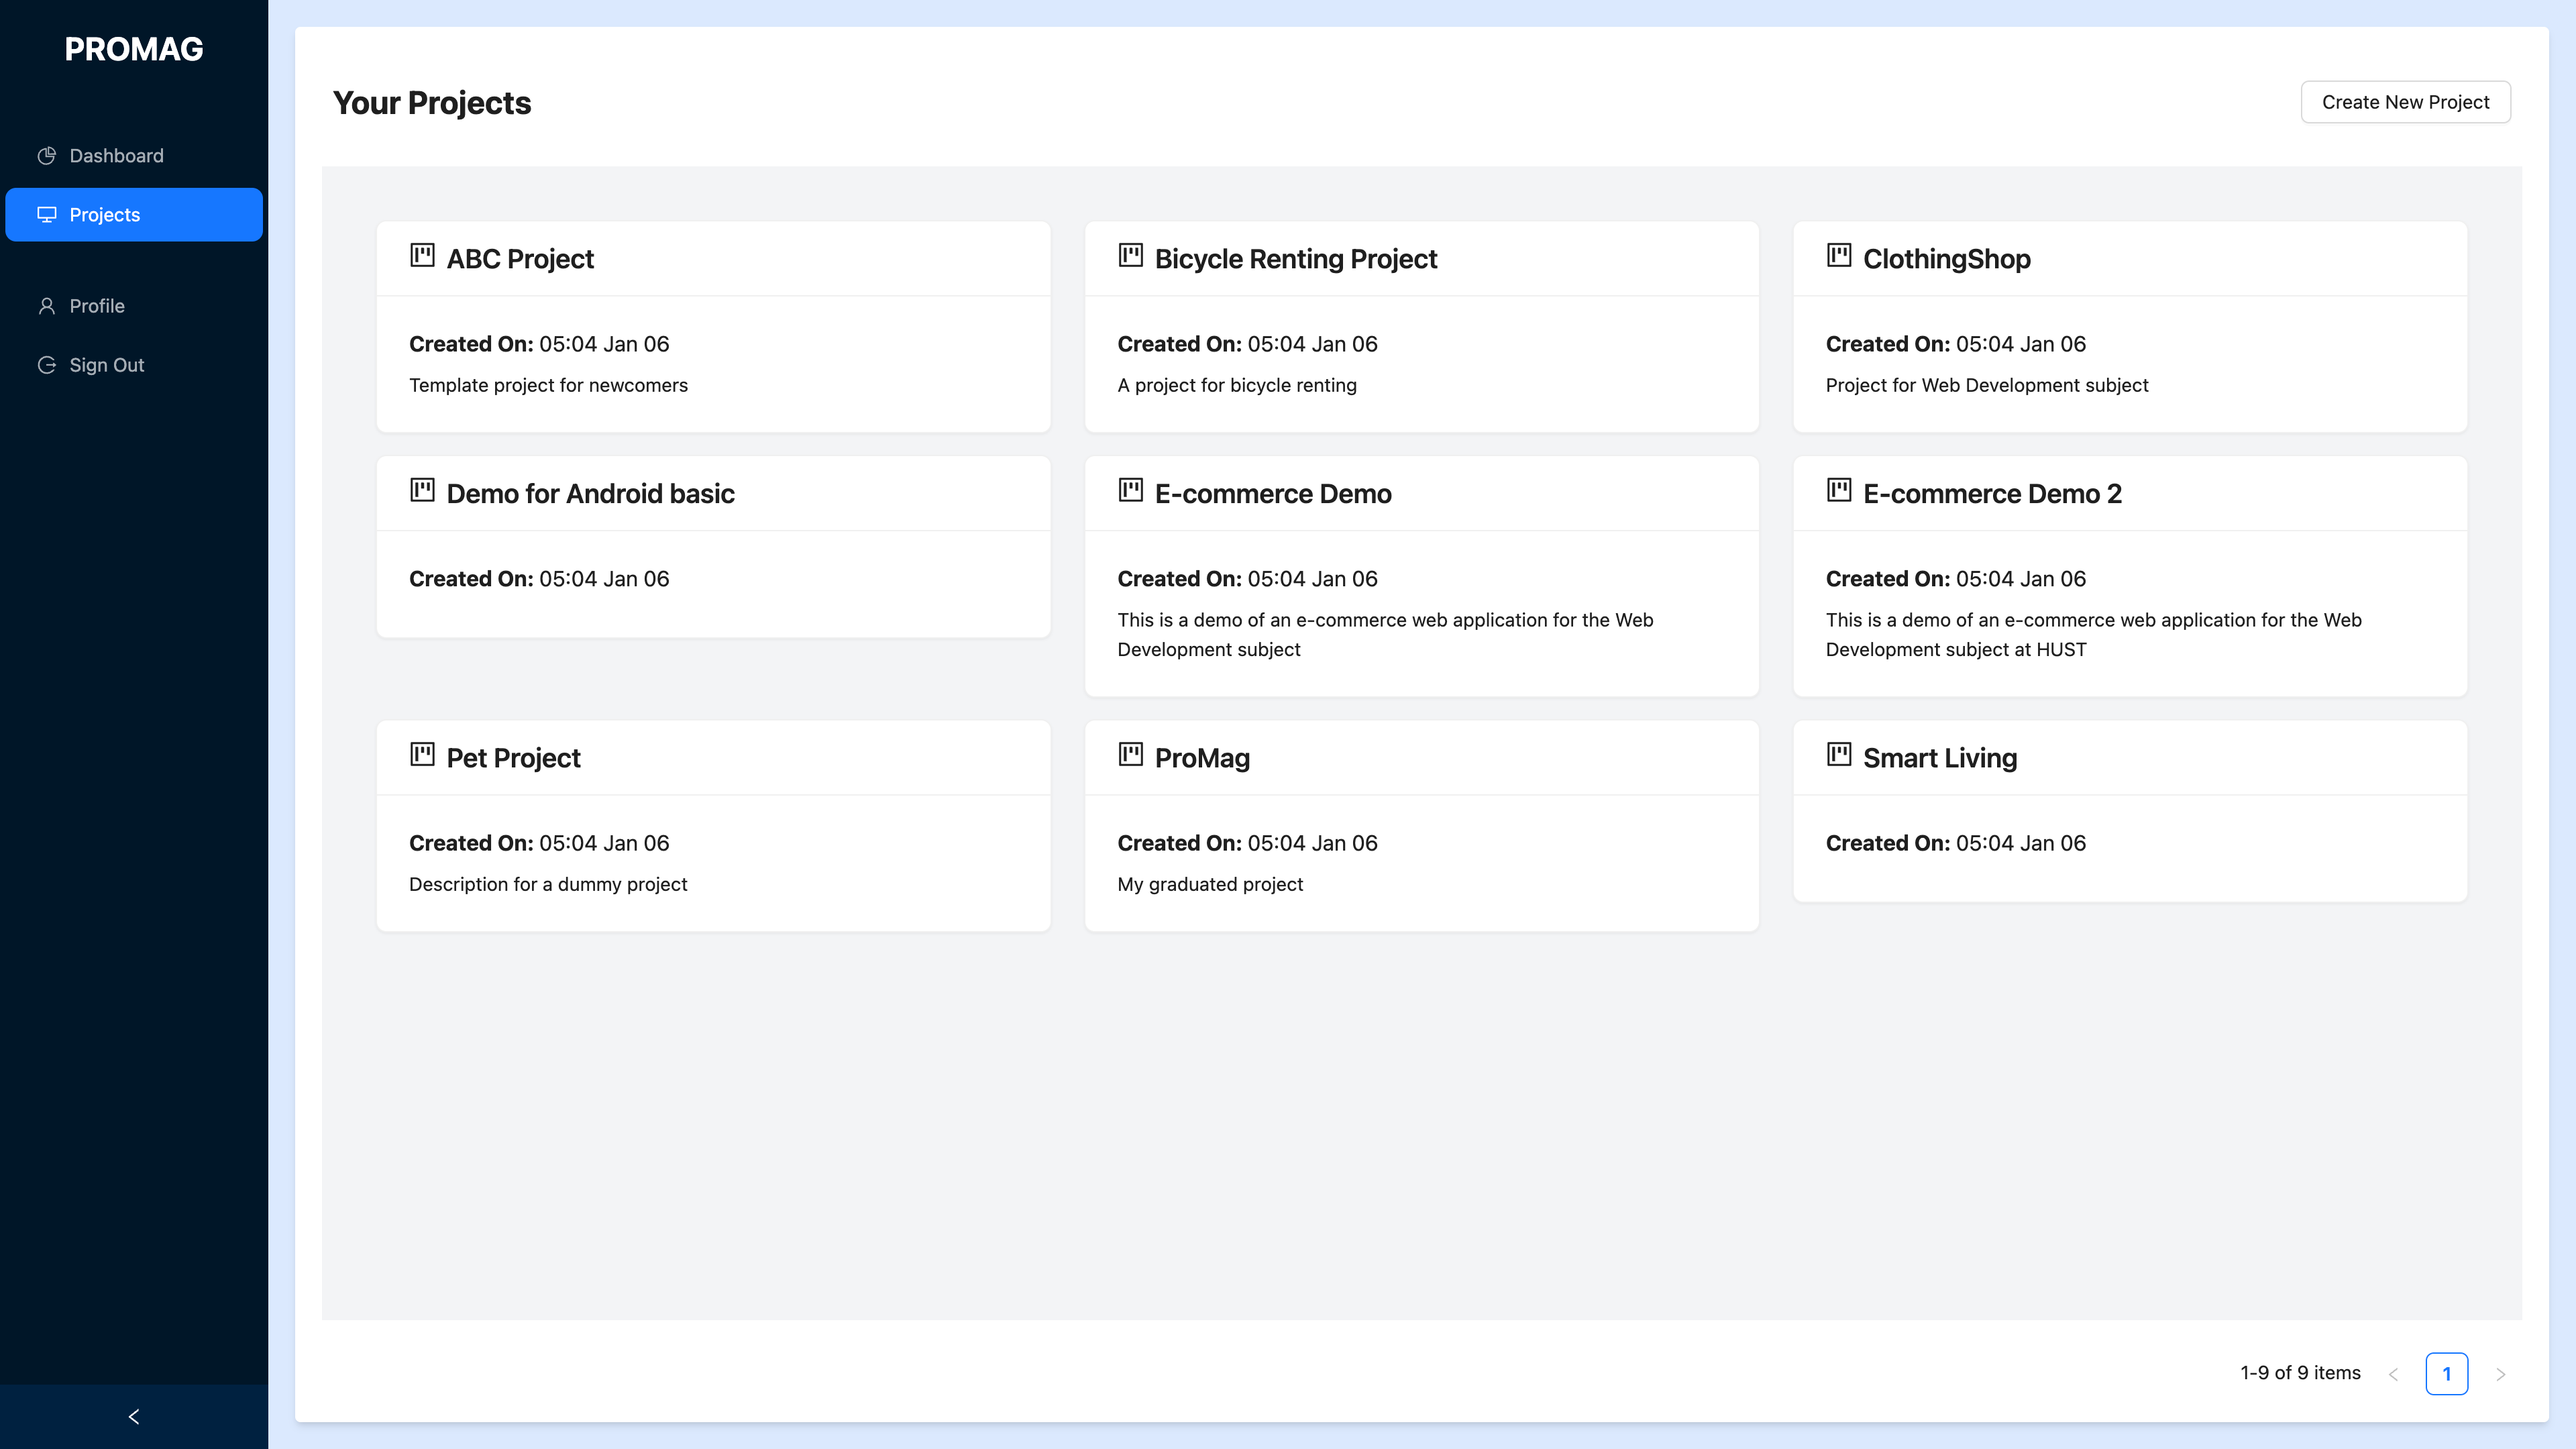
\includegraphics[width=1.0\linewidth]{Hinhve/Screenshot_ProjectList.png}
    \caption{Minh hoạ giao diện Danh sách dự án}
    \label{fig:Screenshot_ProjectList}
\end{figure}

\begin{figure}[H]
    \centering
    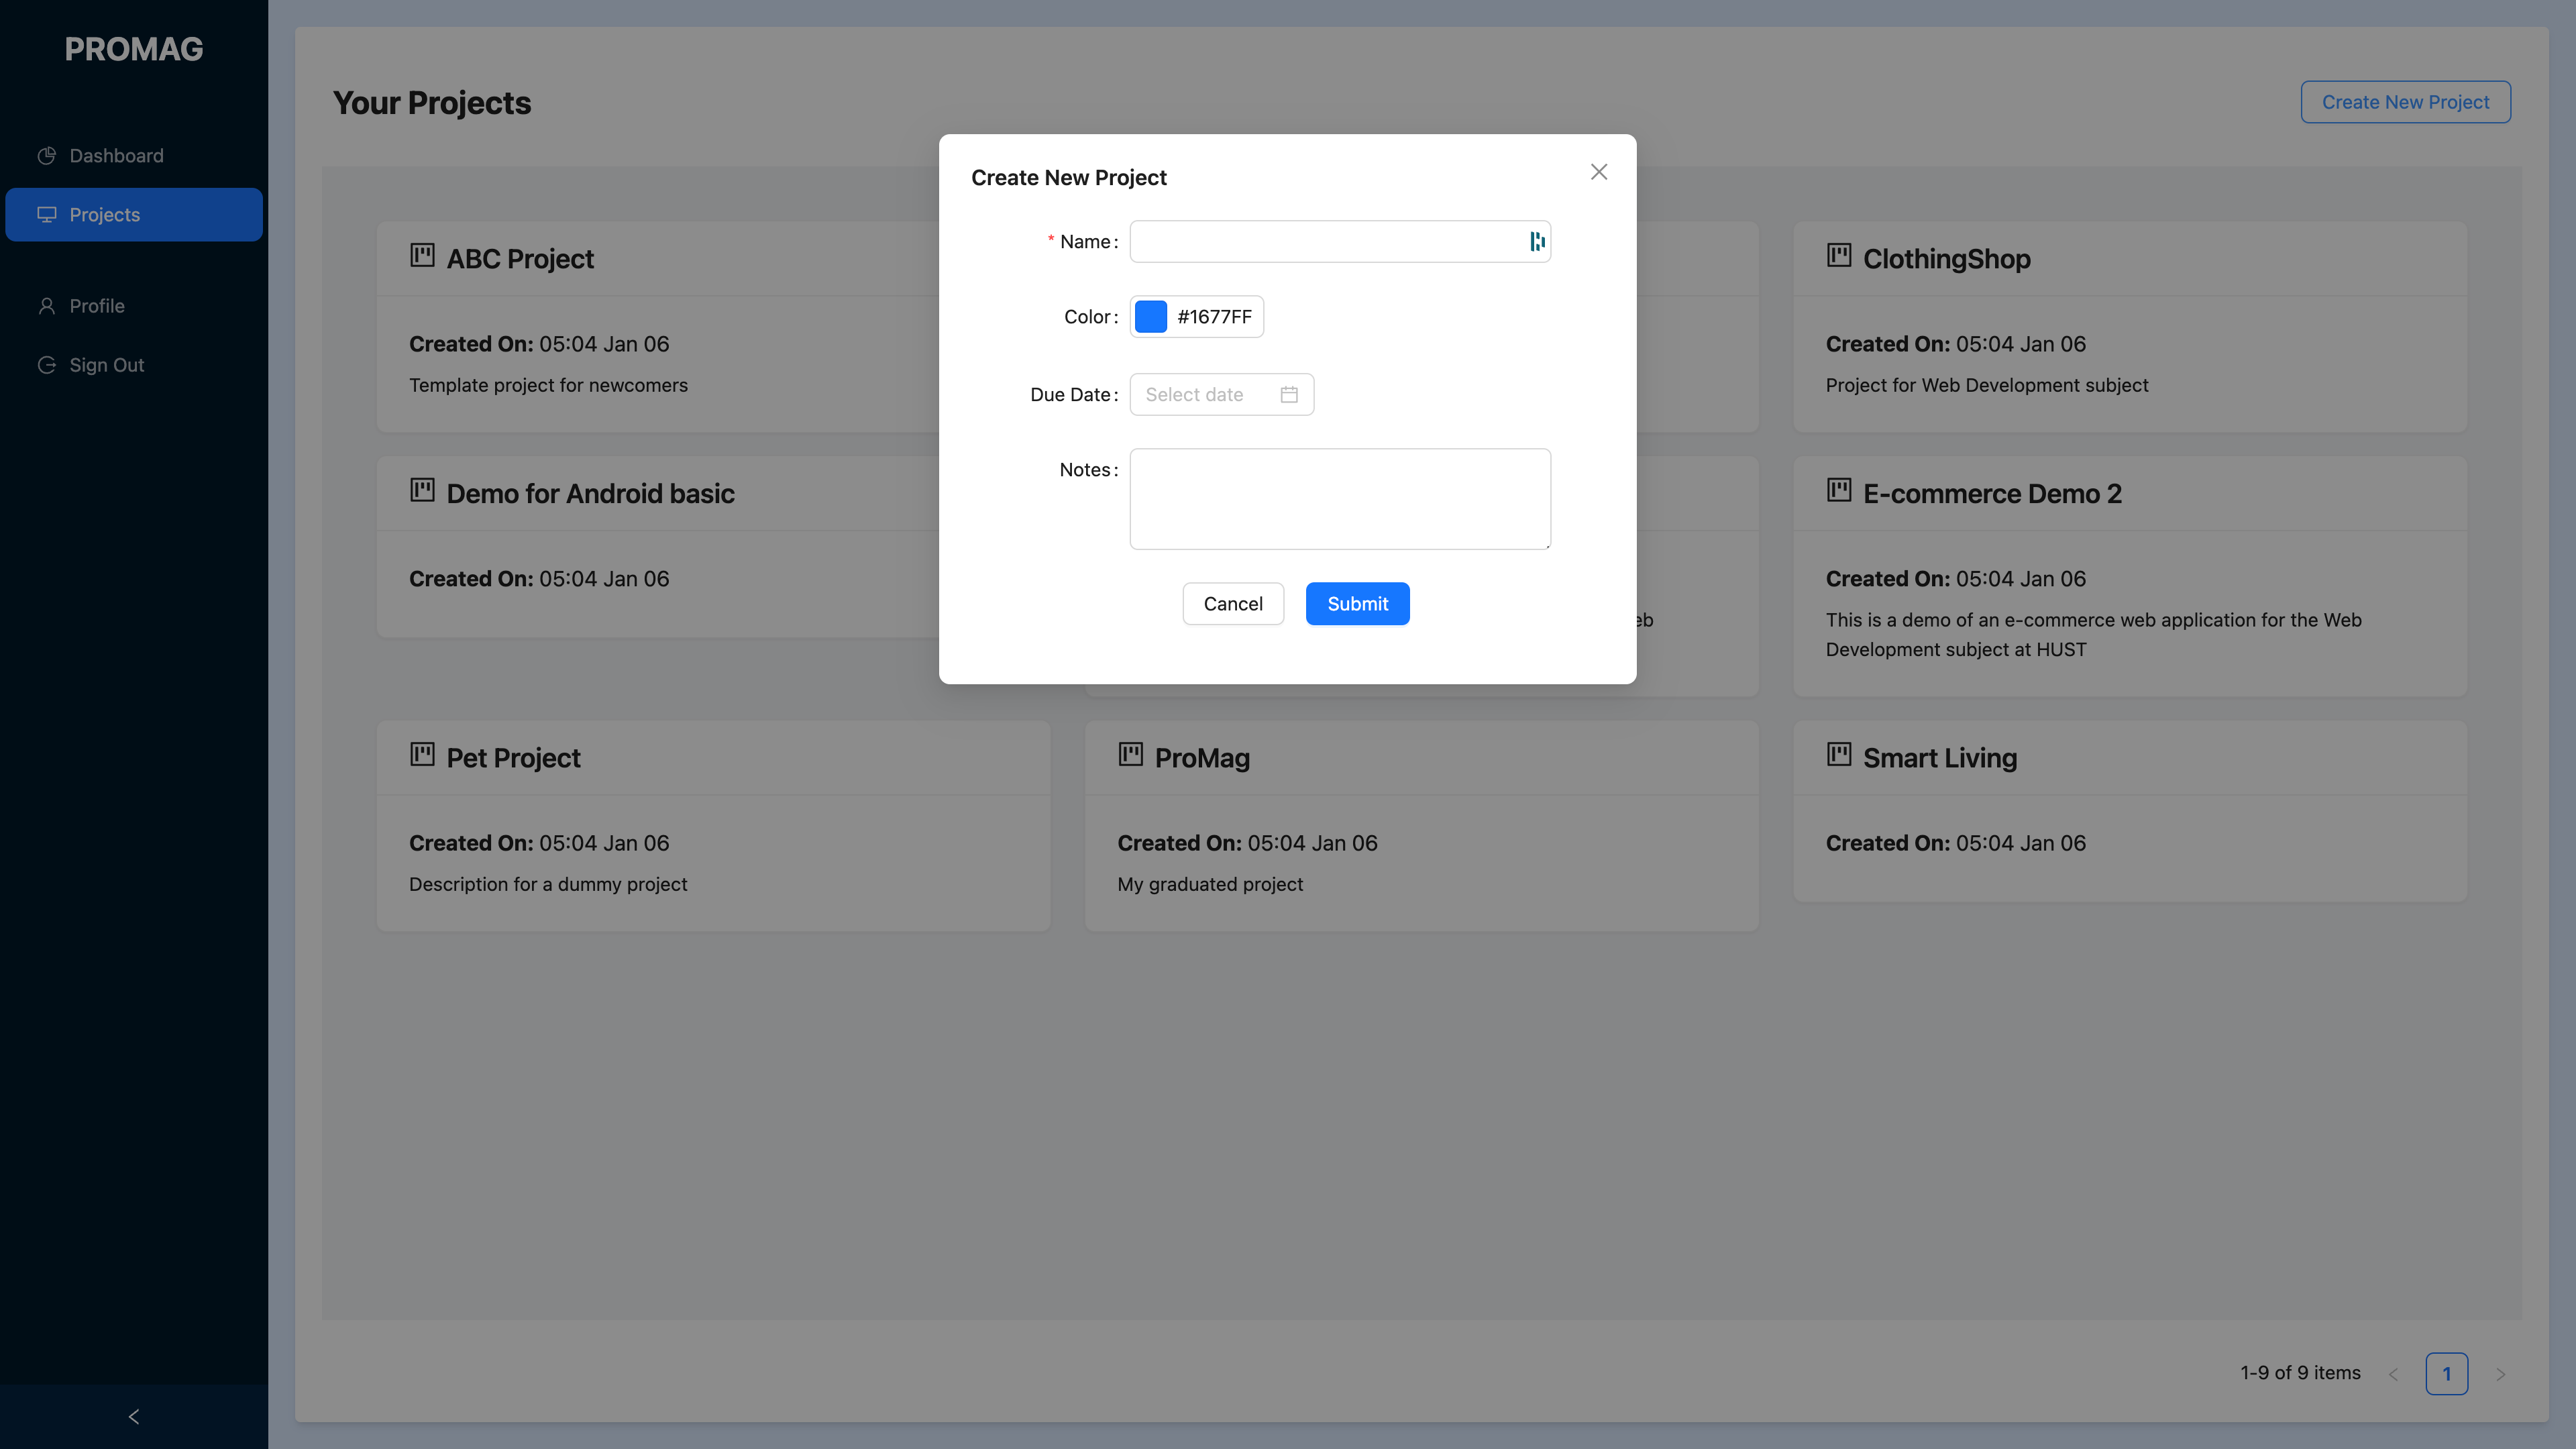
\includegraphics[width=1.0\linewidth]{Hinhve/Screenshot_CreateProject.png}
    \caption{Minh hoạ giao diện Tạo dự án}
    \label{fig:Screenshot_CreateProject}
\end{figure}

\newpage

\begin{figure}[H]
    \centering
    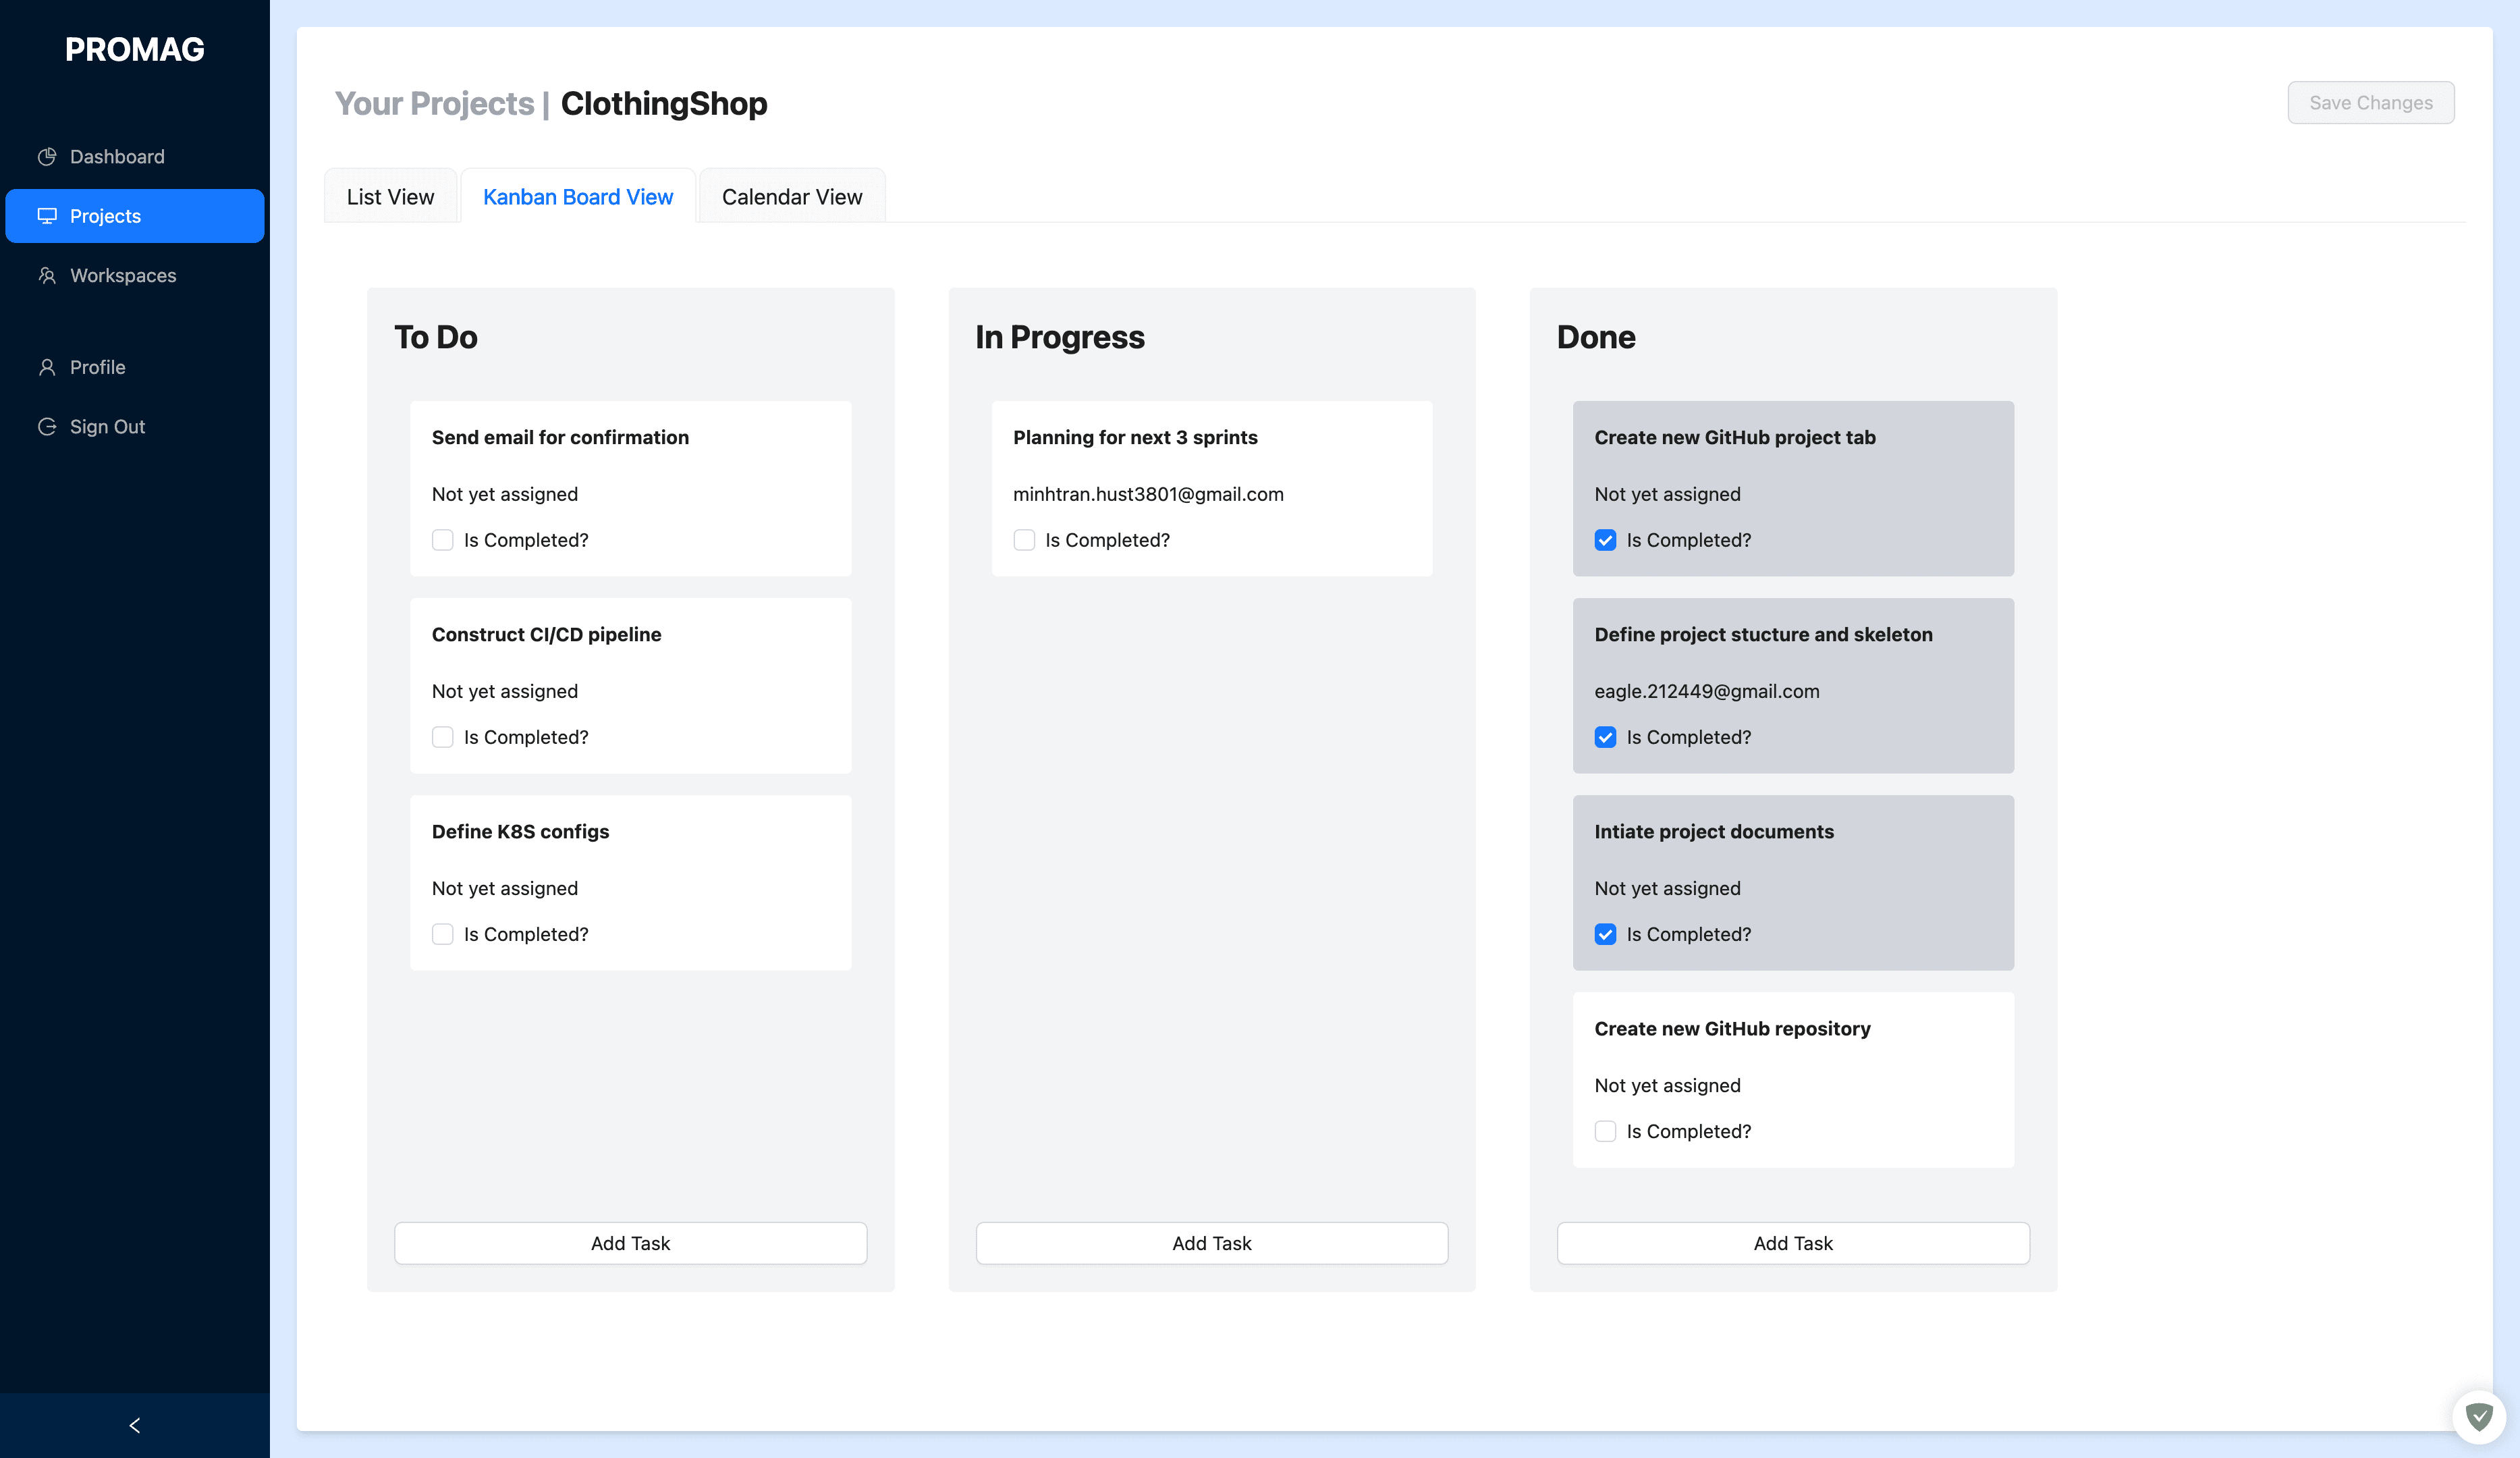
\includegraphics[width=1.0\linewidth]{Hinhve/Screenshot_KanbanBoard.png}
    \caption{Minh hoạ giao diện Chi tiết dự án dạng bảng Kanban}
    \label{fig:Screenshot_KanbanBoard}
\end{figure}

\begin{figure}[H]
    \centering
    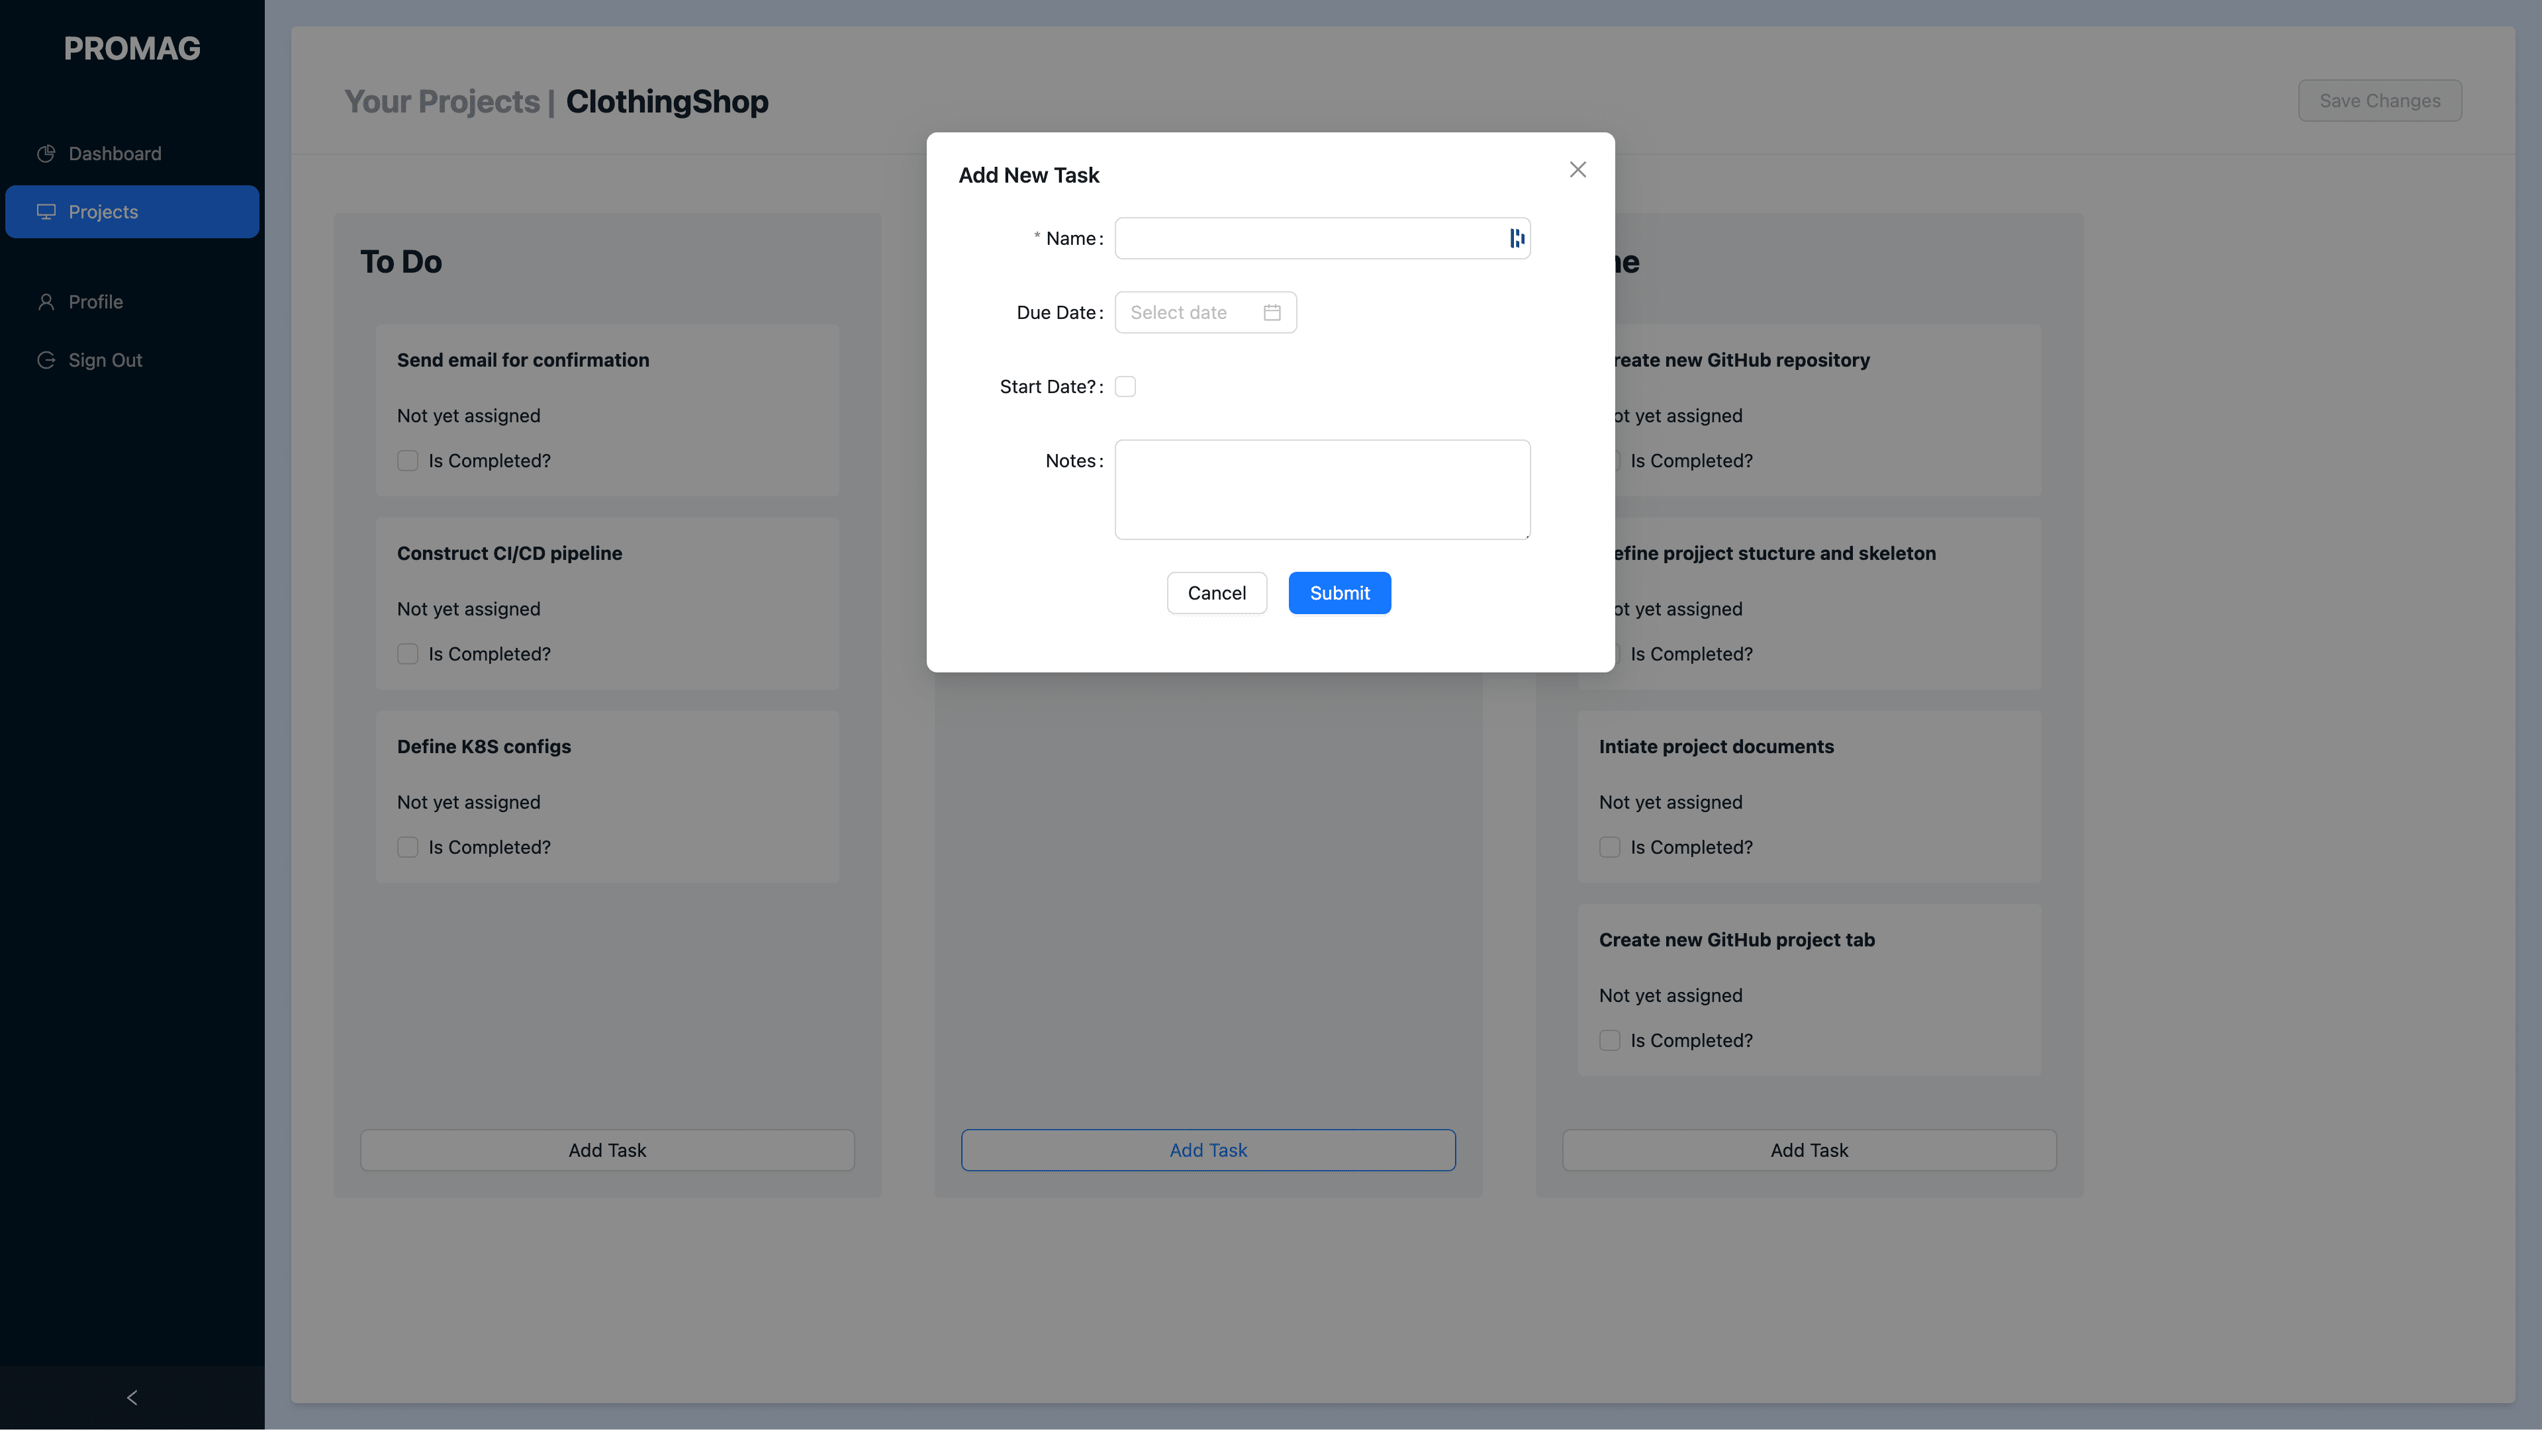
\includegraphics[width=1.0\linewidth]{Hinhve/Screenshot_AddNewTask.png}
    \caption{Minh hoạ giao diện Tạo công việc}
    \label{fig:Screenshot_AddNewTask}
\end{figure}

\newpage

\section{Kiểm thử}
\label{section:4.4}

Trong đồ án này, em đã sử dụng 2 phương pháp kiểm thử chính là kiểm thử hộp đen (Black Box Testing) và kiểm thử đơn vị (Unit Testing). Với kiểm thử hộp đen,
em viết ra các kịch bản kiểm thử dựa trên các chức năng của hệ thống, sau đó thực hiện kiểm thử trên giao diện người dùng. Với kiểm thử đơn vị, em viết các
kịch bản để kiểm thử các hàm, phương thức của các lớp thực hiện giải quyết các yêu cầu nghiệp vụ trong mã nguồn.

\subsection{Kiểm thử chức năng Đăng ký}
\label{subsection:4.4.1}

\begin{table}[H]
    \renewcommand{\arraystretch}{1.2}
    \centering{}
    \begin{tabular}{p{0.3\linewidth}p{0.3\linewidth}p{0.3\linewidth}p{0.1\linewidth}}
        \hline
        \textbf{Kịch bản kiểm thử}                   & \textbf{Kết quả mong muốn}                       & \textbf{Kết quả thực tế}                         & \textbf{Đánh giá} \\ \hline
        Không nhập tên User Name                     & Thông báo: "User Name là trường bắt buộc"        & Thông báo: "User Name là trường bắt buộc"        & Đạt               \\ \hline
        Không nhập địa chỉ Email                     & Thông báo: "Email là trường bắt buộc"            & Thông báo: "Email là trường bắt buộc"            & Đạt               \\ \hline
        Không nhập tên First Name                    & Thông báo: "First Name là trường bắt buộc"       & Thông báo: "First Name là trường bắt buộc"       & Đạt               \\ \hline
        Không nhập tên Last Name                     & Thông báo: "Last Name là trường bắt buộc"        & Thông báo: "Last Name là trường bắt buộc"        & Đạt               \\ \hline
        Không nhập mật khẩu Password                 & Thông báo: "Password là trường bắt buộc"         & Thông báo: "Password là trường bắt buộc"         & Đạt               \\ \hline
        Không nhập lại mật khẩu Password Confirm     & Thông báo: "Password Confirm là trường bắt buộc" & Thông báo: "Password Confirm là trường bắt buộc" & Đạt               \\ \hline
        Nhập địa chỉ Email không có ký tự "@"        & Thông báo: "Địa chỉ Email sai cú pháp"           & Thông báo: "Địa chỉ Email sai cú pháp"           & Đạt               \\ \hline
        Nhập địa chỉ Email đã tồn tại trong hệ thống & Thông báo: "Địa chỉ Email đã được sử dụng"       & Thông báo: "Địa chỉ Email đã được sử dụng"       & Đạt               \\ \hline
        Nhập tên User Name chứa ký tự "@"            & Thông báo: "Tên User Name sai cú pháp"           & Thông báo: "Tên User Name sai cú pháp"           & Đạt               \\ \hline
        Nhập tên User Name đã tồn tại trong hệ thống & Thông báo: "Tên User Name đã được sử dụng"       & Thông báo: "Tên User Name đã được sử dụng"       & Đạt               \\ \hline
    \end{tabular}
    \renewcommand{\arraystretch}{1}
    \caption{Các kịch bản kiểm thử chức năng Đăng ký}
    \label{fig:testcase_register}
\end{table}

\newpage

\subsection{Kiểm thử chức năng Tạo công việc và cập nhật công việc}
\label{subsection:4.4.2}

\begin{table}[H]
    \renewcommand{\arraystretch}{1.2}
    \centering{}
    \begin{tabular}{p{0.3\linewidth}p{0.3\linewidth}p{0.3\linewidth}p{0.1\linewidth}}
        \hline
        \textbf{Kịch bản kiểm thử}                              & \textbf{Kết quả mong muốn}                               & \textbf{Kết quả thực tế}                                 & \textbf{Đánh giá} \\ \hline
        Không nhập tên công việc                                & Thông báo: "Name là trường bắt buộc"                     & Thông báo: "Name là trường bắt buộc"                     & Đạt               \\ \hline
        Không nhập trạng thái ban đầu                           & Thông báo: "Section là trường bắt buộc"                  & Thông báo: "Section là trường bắt buộc"                  & Đạt               \\ \hline
        Gán tập đính kèm có dung lượng lớn hơn 5 MiB            & Thông báo: "Tập đính kèm quá dung lượng giới hạn 5 Mib"  & Thông báo: "Tập đính kèm quá dung lượng giới hạn 5 Mib"  & Đạt               \\ \hline
        Gán tập đính kèm có đuôi .exe                           & Thông báo: "Tập đính kèm có đuôi không hỗ trợ"           & Thông báo: "Tập đính kèm có đuôi không hỗ trợ"           & Đạt               \\ \hline
        Gán tập đính kèm có tên chứa ký tự "@"                  & Thông báo: "Tên tập đính kèm sai cú pháp"                & Thông báo: "Tên tập đính kèm sai cú pháp"                & Đạt               \\ \hline
        Giao công việc cho người dùng không thuộc dự án         & Thông báo: "Người dùng được gán không có quyền truy cập" & Thông báo: "Người dùng được gán không có quyền truy cập" & Đạt               \\ \hline
        Giao công việc cho người dùng không thuộc đội thực hiện & Thông báo: "Người dùng được gán không có quyền truy cập" & Thông báo: "Người dùng được gán không có quyền truy cập" & Đạt               \\ \hline
        Nhập ngày bắt đầu sau ngày tới hạn                      & Thông báo: "Ngày bắt đầu không thoả mãn"                 & Thông báo: "Ngày bắt đầu không thoả mãn"                 & Đạt               \\ \hline
    \end{tabular}
    \renewcommand{\arraystretch}{1}
    \caption{Các kịch bản kiểm thử chức năng Tạo công việc và cập nhật công việc}
    \label{fig:testcase_task}
\end{table}

\newpage

\section{Triển khai}
\label{section:4.5}
\subsection{Ứng dụng Front-end}
\label{subsection:4.5.1}
Đối với ứng dụng Front-end, mã nguồn được lưu trữ trên GitHub và triển khai trên môi trường của Vercel. Trong đó, GitHub là một dịch vụ lưu trữ mã nguồn phổ biến nhất
hiện nay, cung cấp các tính năng cơ bản về quản lý mã nguồn và quản lý phiên bản, cũng như tích hợp tốt với các dịch vụ đám mây khác. Còn Vercel là một nền tảng đám mây
cho phép triển khai các ứng dụng web một cách nhanh chóng, đơn giản và cung cấp sẵn tính năng tự động tích hợp và triển khai ứng dụng (Countinous Integration and Delivery - CI/CD) với GitHub.
Mọi thay đổi tới mã nguồn trên GitHub đều được Vercel tự động nhận biết và triển khai lại ứng dụng một cách tự động.

\subsection{Hệ thống Back-end}
\label{subsection:4.5.2}
Đối với hệ thống Back-end, mã nguồn được lưu trữ trên GitHub và triển khai trên môi trường của Google Cloud Platform. Cụ thể hơn, hệ thống sử dụng
Google Kubernetes Engine với các dịch vụ hỗ trợ bao gồm Google Certificates Manager, Google Cloud Storage. Google Kubernetes Engine là một dịch vụ quản lý
Kubernetes được cung cấp bởi Google Cloud Platform, nó cung cấp một môi trường chạy ứng dụng đám mây, có khả năng mở rộng và có khả năng chịu lỗi cao.

\begin{table}[H]
    \renewcommand{\arraystretch}{1.2}
    \centering{}
    \begin{tabular}{p{0.6\linewidth}p{0.4\linewidth}}
        \hline
        \textbf{Thành phần} & \textbf{Thông số}      \\ \hline
        CPU                 & 8 vCPU                 \\ \hline
        RAM                 & 16 GB                  \\ \hline
        Hệ điều hành        & Container-Optimized OS \\ \hline
        Ổ cứng              & 100 GB                 \\ \hline
    \end{tabular}
    \renewcommand{\arraystretch}{1}
    \caption{Cấu hình dịch vụ Google Kubernetes Engine}
    \label{fig:my_label}
\end{table}

\end{document}
